% !TeX program = xelatex
% !TeX encoding = UTF-8
%
% Bachelor/master thesis -- main file.
% Compile with XeLaTeX + BibTeX:
%   xelatex diplomski.tex
%   bibtex diplomski
%   xelatex diplomski.tex
%   xelatex diplomski.tex     (run again to resolve TOC /references)
%
\documentclass{ftndiplomski}
\usepackage{amsmath}
\usepackage{amssymb}
\usepackage{tikz}
\usepackage{placeins}
\usepackage{float}
\usetikzlibrary{arrows.meta, positioning, shapes.geometric, fit, calc}
\usepackage{subcaption}
% Class options (optional):
%   [twoside]         -- two-sided document, chapters start on odd pages
%   [onehalfspacing]  -- 1.5 line spacing instead of single
%   [serbian]         -- write the thesis in Serbian, Cyrillic script
%   [serbianlatin]    -- write the thesis in Serbian, Latin script
% (default, no option needed: English)

%% =====================================================================
%%  THESIS METADATA -- fill in before writing
%% =====================================================================
\autor{Papp Tamás}
\naslov{Fraktal renderovanje sa hibridnom paralelizacijom}
\naslovEN{Fractal rendering with hybrid parallelism}
\vrstarada{Bachelor Thesis}
\studije{Bachelor Academic Studies}
\mesto{Novi Sad}
\godina{2026}

\studijskiprogram{Compute and Control Engineering}
\brojindeksa{RA 4/2022}
\oblast{Software Engineering}

\mentor{Dr Velko Petrović}
\mentorEN{Dr Velko Petrović, PhD}

\naucnaoblastEN{Software Engineering and Information Technologies}
\naucnadisciplinaEN{Software Engineering}

\keywords{fractal, high performance computing, hybrid systems}
\izvod{One paragraph that captures the essence of the thesis: the
  problem, the motivation, an outline of the solution and the result.}
\abstractEN{One paragraph that captures the essence of the thesis: the
  problem, the motivation, an outline of the solution and the result.}

% Number of chapters, pages, references, tables, figures, graphs, appendixes
\fizickiopis{8}{XX}{X}{X}{X}{X}{X}

\predsednikkomisijeEN{Name Surname, full professor, PhD}
\clankomisijeEN{Name Surname, full professor, PhD}
\datumprihvatanja{}
\datumodbrane{}

%% =====================================================================
\begin{document}

\maketitle

\clearpage
\thispagestyle{empty}
\tableofcontents

\clearpage
\setcounter{page}{1}

\chapter{Introduction}
\label{ch:intro}

\section{Motivation}
\label{sec:motivation}

Fractals are one of the more interesting corners of mathematics. A shape such as the Mandelbrot
set is defined by a short, simple rule, yet applying that rule over and overproduces a boundary
of unlimited detail \cite{mandelbrot1982}. The same kind of structure shows up outside pure math,
in coastlines, in heartbeats, in financial markets, and it has practical uses in data compression,
network design, and medical imaging.

Rendering a fractal such as the Mandelbrot set relies on the escape time algorithm. For each pixel,
a short numerical loop runs until the value either grows past a fixed bound or a maximum iteration
count is reached. One pixel's computation does not depend on any other pixel's result, so the whole
image can, in principle, be computed in parallel. In practice, most fractal rendering software
available to the public still processes pixels one at a time on a single CPU thread, leaving the
rest of the CPU's cores and the GPU idle. Software that does use the GPU rarely also uses the CPU
at the same time. When it does use the CPU, that is usually only as a fallback for machines without
a supported GPU, not as an extra source of compute.

Whether the GPU is actually the faster option is not as settled as it looks. Naive, single threaded
CPU code makes GPU speedups look larger than they are, so a fair comparison has to start from a
properly optimised CPU baseline \cite{lee2010debunking}. A typical personal computer already has a
multicore CPU with SIMD instructions and a GPU sitting next to each other. Using only one of them
wastes hardware the user already owns. That is the motivation for this thesis. It sets out to build
a renderer that pushes the CPU path and the GPU path each as far as they go on their own. It then
combines them with a scheduler that splits the work between CPU and GPU based on which one is
actually faster for a given part of the image \cite{luk2009qilin}. That replaces the usual approach
of treating "CPU renderer" and "GPU renderer" as two separate programs.

\section{Goals}
\label{sec:goals}

The goal of this thesis is to render the Mandelbrot set as fast as possible on a single personal
computer, using the CPU and the GPU together rather than either one alone. Reaching that goal
means working through several smaller objectives, each covered by a later chapter.

The first is the CPU renderer itself. Starting from a scalar escape time baseline, the thesis adds
multicore parallelism, SIMD (\texttt{f64x4}, \texttt{f32x8}), and geometric early exit tests, the
cardioid and period 2 and period 3 checks, that skip the iteration loop for pixels already known to
lie inside the set. On top of that, the distance estimation method and Mariani--Silver boundary
subdivision cut down wasted iteration work by filling large uniform regions of the image without
iterating every pixel in them. Tiled traversal ordered by Hilbert or Morton curves further improves
memory access locality. A separate concern is deep zooming. Plain double precision arithmetic runs
out of precision long before an interesting zoom level is reached. The renderer therefore also needs
perturbation theory, using a single reference orbit or multiple reference orbits with rebasing,
series approximation, and double-double arithmetic to stay accurate and fast
\cite{heilandallen2021deepzoom}.

The second objective is the GPU side. It means implementing the same escape time kernels as GPU
compute shaders, once portably with wgpu and WebGPU and once as a hand tuned CUDA backend. Each
implementation uses a traversal order and memory layout suited to the GPU rather than porting
directly from the CPU code.

The third objective ties the first two together. A hybrid CPU and GPU scheduler splits a frame
into tiles, classifies each tile by expected cost, and distributes tiles across CPU worker threads
and the GPU at the same time. It then adjusts the split at runtime with a feedback PI controller
driven by the measured throughput of each device.

The fourth objective is to measure all of this properly, since none of the above is worth much
without evidence. That means fixing a benchmarking setup, the hardware, the benchmark scenes at
shallow and deep zoom, and the throughput and latency metrics. It then means measuring what each
optimisation actually contributes and comparing the CPU only, GPU only, and hybrid configurations
against each other and against existing open source fractal renderers. This last comparison
matters on its own. A hybrid scheduler is only worth its added complexity if it measurably beats
running the CPU and GPU renderers separately.

\chapter{Background}
\label{ch:background}

\section{Fractals, General Concepts and Applications}
\label{sec:fractal-concepts}

Before narrowing to the Mandelbrot set specifically, it is worth saying what a fractal actually is
in general. A fractal is a shape whose complexity does not go away under magnification. A circle
looks more and more like a straight line the closer it is examined, but a fractal keeps showing
structure at every scale, and small pieces of it resemble the whole shape, either exactly or in a
statistical sense \cite{mandelbrot1982}. The Koch curve, the Sierpinski triangle, the Vicsek
fractal, and the Sierpinski carpet, shown in Figure~\ref{fig:fractal-examples}, are four of the
classic examples. Each is built by repeating a simple replacement rule on a starting shape, over,
and over, without end.

\begin{figure}[H]
  \centering
  \begin{subfigure}[b]{0.45\textwidth}
    \centering
    
\begin{tikzpicture}[x=5cm,y=5cm]
      \draw[thick] plot coordinates {(0.00000,0.00000) (0.01235,0.00000) (0.01852,0.01069) (0.02469,0.00000) (0.03704,0.00000) (0.04321,0.01069) (0.03704,0.02138) (0.04938,0.02138) (0.05556,0.03208) (0.06173,0.02138) (0.07407,0.02138) (0.06790,0.01069) (0.07407,0.00000) (0.08642,0.00000) (0.09259,0.01069) (0.09877,0.00000) (0.11111,0.00000) (0.11728,0.01069) (0.11111,0.02138) (0.12346,0.02138) (0.12963,0.03208) (0.12346,0.04277) (0.11111,0.04277) (0.11728,0.05346) (0.11111,0.06415) (0.12346,0.06415) (0.12963,0.07484) (0.13580,0.06415) (0.14815,0.06415) (0.15432,0.07484) (0.14815,0.08553) (0.16049,0.08553) (0.16667,0.09623) (0.17284,0.08553) (0.18519,0.08553) (0.17901,0.07484) (0.18519,0.06415) (0.19753,0.06415) (0.20370,0.07484) (0.20988,0.06415) (0.22222,0.06415) (0.21605,0.05346) (0.22222,0.04277) (0.20988,0.04277) (0.20370,0.03208) (0.20988,0.02138) (0.22222,0.02138) (0.21605,0.01069) (0.22222,0.00000) (0.23457,0.00000) (0.24074,0.01069) (0.24691,0.00000) (0.25926,0.00000) (0.26543,0.01069) (0.25926,0.02138) (0.27160,0.02138) (0.27778,0.03208) (0.28395,0.02138) (0.29630,0.02138) (0.29012,0.01069) (0.29630,0.00000) (0.30864,0.00000) (0.31481,0.01069) (0.32099,0.00000) (0.33333,0.00000) (0.33951,0.01069) (0.33333,0.02138) (0.34568,0.02138) (0.35185,0.03208) (0.34568,0.04277) (0.33333,0.04277) (0.33951,0.05346) (0.33333,0.06415) (0.34568,0.06415) (0.35185,0.07484) (0.35802,0.06415) (0.37037,0.06415) (0.37654,0.07484) (0.37037,0.08553) (0.38272,0.08553) (0.38889,0.09623) (0.38272,0.10692) (0.37037,0.10692) (0.37654,0.11761) (0.37037,0.12830) (0.35802,0.12830) (0.35185,0.11761) (0.34568,0.12830) (0.33333,0.12830) (0.33951,0.13899) (0.33333,0.14968) (0.34568,0.14968) (0.35185,0.16038) (0.34568,0.17107) (0.33333,0.17107) (0.33951,0.18176) (0.33333,0.19245) (0.34568,0.19245) (0.35185,0.20314) (0.35802,0.19245) (0.37037,0.19245) (0.37654,0.20314) (0.37037,0.21383) (0.38272,0.21383) (0.38889,0.22453) (0.39506,0.21383) (0.40741,0.21383) (0.40123,0.20314) (0.40741,0.19245) (0.41975,0.19245) (0.42593,0.20314) (0.43210,0.19245) (0.44444,0.19245) (0.45062,0.20314) (0.44444,0.21383) (0.45679,0.21383) (0.46296,0.22453) (0.45679,0.23522) (0.44444,0.23522) (0.45062,0.24591) (0.44444,0.25660) (0.45679,0.25660) (0.46296,0.26729) (0.46914,0.25660) (0.48148,0.25660) (0.48765,0.26729) (0.48148,0.27798) (0.49383,0.27798) (0.50000,0.28868) (0.50617,0.27798) (0.51852,0.27798) (0.51235,0.26729) (0.51852,0.25660) (0.53086,0.25660) (0.53704,0.26729) (0.54321,0.25660) (0.55556,0.25660) (0.54938,0.24591) (0.55556,0.23522) (0.54321,0.23522) (0.53704,0.22453) (0.54321,0.21383) (0.55556,0.21383) (0.54938,0.20314) (0.55556,0.19245) (0.56790,0.19245) (0.57407,0.20314) (0.58025,0.19245) (0.59259,0.19245) (0.59877,0.20314) (0.59259,0.21383) (0.60494,0.21383) (0.61111,0.22453) (0.61728,0.21383) (0.62963,0.21383) (0.62346,0.20314) (0.62963,0.19245) (0.64198,0.19245) (0.64815,0.20314) (0.65432,0.19245) (0.66667,0.19245) (0.66049,0.18176) (0.66667,0.17107) (0.65432,0.17107) (0.64815,0.16038) (0.65432,0.14968) (0.66667,0.14968) (0.66049,0.13899) (0.66667,0.12830) (0.65432,0.12830) (0.64815,0.11761) (0.64198,0.12830) (0.62963,0.12830) (0.62346,0.11761) (0.62963,0.10692) (0.61728,0.10692) (0.61111,0.09623) (0.61728,0.08553) (0.62963,0.08553) (0.62346,0.07484) (0.62963,0.06415) (0.64198,0.06415) (0.64815,0.07484) (0.65432,0.06415) (0.66667,0.06415) (0.66049,0.05346) (0.66667,0.04277) (0.65432,0.04277) (0.64815,0.03208) (0.65432,0.02138) (0.66667,0.02138) (0.66049,0.01069) (0.66667,0.00000) (0.67901,0.00000) (0.68519,0.01069) (0.69136,0.00000) (0.70370,0.00000) (0.70988,0.01069) (0.70370,0.02138) (0.71605,0.02138) (0.72222,0.03208) (0.72840,0.02138) (0.74074,0.02138) (0.73457,0.01069) (0.74074,0.00000) (0.75309,0.00000) (0.75926,0.01069) (0.76543,0.00000) (0.77778,0.00000) (0.78395,0.01069) (0.77778,0.02138) (0.79012,0.02138) (0.79630,0.03208) (0.79012,0.04277) (0.77778,0.04277) (0.78395,0.05346) (0.77778,0.06415) (0.79012,0.06415) (0.79630,0.07484) (0.80247,0.06415) (0.81481,0.06415) (0.82099,0.07484) (0.81481,0.08553) (0.82716,0.08553) (0.83333,0.09623) (0.83951,0.08553) (0.85185,0.08553) (0.84568,0.07484) (0.85185,0.06415) (0.86420,0.06415) (0.87037,0.07484) (0.87654,0.06415) (0.88889,0.06415) (0.88272,0.05346) (0.88889,0.04277) (0.87654,0.04277) (0.87037,0.03208) (0.87654,0.02138) (0.88889,0.02138) (0.88272,0.01069) (0.88889,0.00000) (0.90123,0.00000) (0.90741,0.01069) (0.91358,0.00000) (0.92593,0.00000) (0.93210,0.01069) (0.92593,0.02138) (0.93827,0.02138) (0.94444,0.03208) (0.95062,0.02138) (0.96296,0.02138) (0.95679,0.01069) (0.96296,0.00000) (0.97531,0.00000) (0.98148,0.01069) (0.98765,0.00000) (1.00000,0.00000)};

    \end{tikzpicture}
    \caption{Koch curve}
  \end{subfigure}
  \hfill
  \begin{subfigure}[b]{0.45\textwidth}
    \centering
    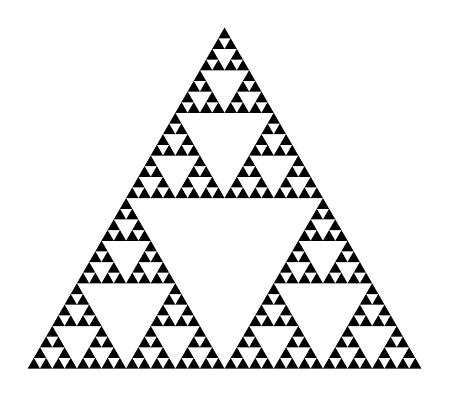
\begin{tikzpicture}[x=5cm,y=5cm]
      \fill (0.00000,0.00000) -- (0.03125,0.00000) -- (0.01562,0.02706) -- cycle;
\fill (0.03125,0.00000) -- (0.06250,0.00000) -- (0.04688,0.02706) -- cycle;
\fill (0.01562,0.02706) -- (0.04688,0.02706) -- (0.03125,0.05413) -- cycle;
\fill (0.06250,0.00000) -- (0.09375,0.00000) -- (0.07812,0.02706) -- cycle;
\fill (0.09375,0.00000) -- (0.12500,0.00000) -- (0.10938,0.02706) -- cycle;
\fill (0.07812,0.02706) -- (0.10938,0.02706) -- (0.09375,0.05413) -- cycle;
\fill (0.03125,0.05413) -- (0.06250,0.05413) -- (0.04688,0.08119) -- cycle;
\fill (0.06250,0.05413) -- (0.09375,0.05413) -- (0.07812,0.08119) -- cycle;
\fill (0.04688,0.08119) -- (0.07812,0.08119) -- (0.06250,0.10825) -- cycle;
\fill (0.12500,0.00000) -- (0.15625,0.00000) -- (0.14062,0.02706) -- cycle;
\fill (0.15625,0.00000) -- (0.18750,0.00000) -- (0.17188,0.02706) -- cycle;
\fill (0.14062,0.02706) -- (0.17188,0.02706) -- (0.15625,0.05413) -- cycle;
\fill (0.18750,0.00000) -- (0.21875,0.00000) -- (0.20312,0.02706) -- cycle;
\fill (0.21875,0.00000) -- (0.25000,0.00000) -- (0.23438,0.02706) -- cycle;
\fill (0.20312,0.02706) -- (0.23438,0.02706) -- (0.21875,0.05413) -- cycle;
\fill (0.15625,0.05413) -- (0.18750,0.05413) -- (0.17188,0.08119) -- cycle;
\fill (0.18750,0.05413) -- (0.21875,0.05413) -- (0.20312,0.08119) -- cycle;
\fill (0.17188,0.08119) -- (0.20312,0.08119) -- (0.18750,0.10825) -- cycle;
\fill (0.06250,0.10825) -- (0.09375,0.10825) -- (0.07812,0.13532) -- cycle;
\fill (0.09375,0.10825) -- (0.12500,0.10825) -- (0.10938,0.13532) -- cycle;
\fill (0.07812,0.13532) -- (0.10938,0.13532) -- (0.09375,0.16238) -- cycle;
\fill (0.12500,0.10825) -- (0.15625,0.10825) -- (0.14062,0.13532) -- cycle;
\fill (0.15625,0.10825) -- (0.18750,0.10825) -- (0.17188,0.13532) -- cycle;
\fill (0.14062,0.13532) -- (0.17188,0.13532) -- (0.15625,0.16238) -- cycle;
\fill (0.09375,0.16238) -- (0.12500,0.16238) -- (0.10938,0.18944) -- cycle;
\fill (0.12500,0.16238) -- (0.15625,0.16238) -- (0.14062,0.18944) -- cycle;
\fill (0.10938,0.18944) -- (0.14062,0.18944) -- (0.12500,0.21651) -- cycle;
\fill (0.25000,0.00000) -- (0.28125,0.00000) -- (0.26562,0.02706) -- cycle;
\fill (0.28125,0.00000) -- (0.31250,0.00000) -- (0.29688,0.02706) -- cycle;
\fill (0.26562,0.02706) -- (0.29688,0.02706) -- (0.28125,0.05413) -- cycle;
\fill (0.31250,0.00000) -- (0.34375,0.00000) -- (0.32812,0.02706) -- cycle;
\fill (0.34375,0.00000) -- (0.37500,0.00000) -- (0.35938,0.02706) -- cycle;
\fill (0.32812,0.02706) -- (0.35938,0.02706) -- (0.34375,0.05413) -- cycle;
\fill (0.28125,0.05413) -- (0.31250,0.05413) -- (0.29688,0.08119) -- cycle;
\fill (0.31250,0.05413) -- (0.34375,0.05413) -- (0.32812,0.08119) -- cycle;
\fill (0.29688,0.08119) -- (0.32812,0.08119) -- (0.31250,0.10825) -- cycle;
\fill (0.37500,0.00000) -- (0.40625,0.00000) -- (0.39062,0.02706) -- cycle;
\fill (0.40625,0.00000) -- (0.43750,0.00000) -- (0.42188,0.02706) -- cycle;
\fill (0.39062,0.02706) -- (0.42188,0.02706) -- (0.40625,0.05413) -- cycle;
\fill (0.43750,0.00000) -- (0.46875,0.00000) -- (0.45312,0.02706) -- cycle;
\fill (0.46875,0.00000) -- (0.50000,0.00000) -- (0.48438,0.02706) -- cycle;
\fill (0.45312,0.02706) -- (0.48438,0.02706) -- (0.46875,0.05413) -- cycle;
\fill (0.40625,0.05413) -- (0.43750,0.05413) -- (0.42188,0.08119) -- cycle;
\fill (0.43750,0.05413) -- (0.46875,0.05413) -- (0.45312,0.08119) -- cycle;
\fill (0.42188,0.08119) -- (0.45312,0.08119) -- (0.43750,0.10825) -- cycle;
\fill (0.31250,0.10825) -- (0.34375,0.10825) -- (0.32812,0.13532) -- cycle;
\fill (0.34375,0.10825) -- (0.37500,0.10825) -- (0.35938,0.13532) -- cycle;
\fill (0.32812,0.13532) -- (0.35938,0.13532) -- (0.34375,0.16238) -- cycle;
\fill (0.37500,0.10825) -- (0.40625,0.10825) -- (0.39062,0.13532) -- cycle;
\fill (0.40625,0.10825) -- (0.43750,0.10825) -- (0.42188,0.13532) -- cycle;
\fill (0.39062,0.13532) -- (0.42188,0.13532) -- (0.40625,0.16238) -- cycle;
\fill (0.34375,0.16238) -- (0.37500,0.16238) -- (0.35938,0.18944) -- cycle;
\fill (0.37500,0.16238) -- (0.40625,0.16238) -- (0.39062,0.18944) -- cycle;
\fill (0.35938,0.18944) -- (0.39062,0.18944) -- (0.37500,0.21651) -- cycle;
\fill (0.12500,0.21651) -- (0.15625,0.21651) -- (0.14062,0.24357) -- cycle;
\fill (0.15625,0.21651) -- (0.18750,0.21651) -- (0.17188,0.24357) -- cycle;
\fill (0.14062,0.24357) -- (0.17188,0.24357) -- (0.15625,0.27063) -- cycle;
\fill (0.18750,0.21651) -- (0.21875,0.21651) -- (0.20312,0.24357) -- cycle;
\fill (0.21875,0.21651) -- (0.25000,0.21651) -- (0.23438,0.24357) -- cycle;
\fill (0.20312,0.24357) -- (0.23438,0.24357) -- (0.21875,0.27063) -- cycle;
\fill (0.15625,0.27063) -- (0.18750,0.27063) -- (0.17188,0.29770) -- cycle;
\fill (0.18750,0.27063) -- (0.21875,0.27063) -- (0.20312,0.29770) -- cycle;
\fill (0.17188,0.29770) -- (0.20312,0.29770) -- (0.18750,0.32476) -- cycle;
\fill (0.25000,0.21651) -- (0.28125,0.21651) -- (0.26562,0.24357) -- cycle;
\fill (0.28125,0.21651) -- (0.31250,0.21651) -- (0.29688,0.24357) -- cycle;
\fill (0.26562,0.24357) -- (0.29688,0.24357) -- (0.28125,0.27063) -- cycle;
\fill (0.31250,0.21651) -- (0.34375,0.21651) -- (0.32812,0.24357) -- cycle;
\fill (0.34375,0.21651) -- (0.37500,0.21651) -- (0.35938,0.24357) -- cycle;
\fill (0.32812,0.24357) -- (0.35938,0.24357) -- (0.34375,0.27063) -- cycle;
\fill (0.28125,0.27063) -- (0.31250,0.27063) -- (0.29688,0.29770) -- cycle;
\fill (0.31250,0.27063) -- (0.34375,0.27063) -- (0.32812,0.29770) -- cycle;
\fill (0.29688,0.29770) -- (0.32812,0.29770) -- (0.31250,0.32476) -- cycle;
\fill (0.18750,0.32476) -- (0.21875,0.32476) -- (0.20312,0.35182) -- cycle;
\fill (0.21875,0.32476) -- (0.25000,0.32476) -- (0.23438,0.35182) -- cycle;
\fill (0.20312,0.35182) -- (0.23438,0.35182) -- (0.21875,0.37889) -- cycle;
\fill (0.25000,0.32476) -- (0.28125,0.32476) -- (0.26562,0.35182) -- cycle;
\fill (0.28125,0.32476) -- (0.31250,0.32476) -- (0.29688,0.35182) -- cycle;
\fill (0.26562,0.35182) -- (0.29688,0.35182) -- (0.28125,0.37889) -- cycle;
\fill (0.21875,0.37889) -- (0.25000,0.37889) -- (0.23438,0.40595) -- cycle;
\fill (0.25000,0.37889) -- (0.28125,0.37889) -- (0.26562,0.40595) -- cycle;
\fill (0.23438,0.40595) -- (0.26562,0.40595) -- (0.25000,0.43301) -- cycle;
\fill (0.50000,0.00000) -- (0.53125,0.00000) -- (0.51562,0.02706) -- cycle;
\fill (0.53125,0.00000) -- (0.56250,0.00000) -- (0.54688,0.02706) -- cycle;
\fill (0.51562,0.02706) -- (0.54688,0.02706) -- (0.53125,0.05413) -- cycle;
\fill (0.56250,0.00000) -- (0.59375,0.00000) -- (0.57812,0.02706) -- cycle;
\fill (0.59375,0.00000) -- (0.62500,0.00000) -- (0.60938,0.02706) -- cycle;
\fill (0.57812,0.02706) -- (0.60938,0.02706) -- (0.59375,0.05413) -- cycle;
\fill (0.53125,0.05413) -- (0.56250,0.05413) -- (0.54688,0.08119) -- cycle;
\fill (0.56250,0.05413) -- (0.59375,0.05413) -- (0.57812,0.08119) -- cycle;
\fill (0.54688,0.08119) -- (0.57812,0.08119) -- (0.56250,0.10825) -- cycle;
\fill (0.62500,0.00000) -- (0.65625,0.00000) -- (0.64062,0.02706) -- cycle;
\fill (0.65625,0.00000) -- (0.68750,0.00000) -- (0.67188,0.02706) -- cycle;
\fill (0.64062,0.02706) -- (0.67188,0.02706) -- (0.65625,0.05413) -- cycle;
\fill (0.68750,0.00000) -- (0.71875,0.00000) -- (0.70312,0.02706) -- cycle;
\fill (0.71875,0.00000) -- (0.75000,0.00000) -- (0.73438,0.02706) -- cycle;
\fill (0.70312,0.02706) -- (0.73438,0.02706) -- (0.71875,0.05413) -- cycle;
\fill (0.65625,0.05413) -- (0.68750,0.05413) -- (0.67188,0.08119) -- cycle;
\fill (0.68750,0.05413) -- (0.71875,0.05413) -- (0.70312,0.08119) -- cycle;
\fill (0.67188,0.08119) -- (0.70312,0.08119) -- (0.68750,0.10825) -- cycle;
\fill (0.56250,0.10825) -- (0.59375,0.10825) -- (0.57812,0.13532) -- cycle;
\fill (0.59375,0.10825) -- (0.62500,0.10825) -- (0.60938,0.13532) -- cycle;
\fill (0.57812,0.13532) -- (0.60938,0.13532) -- (0.59375,0.16238) -- cycle;
\fill (0.62500,0.10825) -- (0.65625,0.10825) -- (0.64062,0.13532) -- cycle;
\fill (0.65625,0.10825) -- (0.68750,0.10825) -- (0.67188,0.13532) -- cycle;
\fill (0.64062,0.13532) -- (0.67188,0.13532) -- (0.65625,0.16238) -- cycle;
\fill (0.59375,0.16238) -- (0.62500,0.16238) -- (0.60938,0.18944) -- cycle;
\fill (0.62500,0.16238) -- (0.65625,0.16238) -- (0.64062,0.18944) -- cycle;
\fill (0.60938,0.18944) -- (0.64062,0.18944) -- (0.62500,0.21651) -- cycle;
\fill (0.75000,0.00000) -- (0.78125,0.00000) -- (0.76562,0.02706) -- cycle;
\fill (0.78125,0.00000) -- (0.81250,0.00000) -- (0.79688,0.02706) -- cycle;
\fill (0.76562,0.02706) -- (0.79688,0.02706) -- (0.78125,0.05413) -- cycle;
\fill (0.81250,0.00000) -- (0.84375,0.00000) -- (0.82812,0.02706) -- cycle;
\fill (0.84375,0.00000) -- (0.87500,0.00000) -- (0.85938,0.02706) -- cycle;
\fill (0.82812,0.02706) -- (0.85938,0.02706) -- (0.84375,0.05413) -- cycle;
\fill (0.78125,0.05413) -- (0.81250,0.05413) -- (0.79688,0.08119) -- cycle;
\fill (0.81250,0.05413) -- (0.84375,0.05413) -- (0.82812,0.08119) -- cycle;
\fill (0.79688,0.08119) -- (0.82812,0.08119) -- (0.81250,0.10825) -- cycle;
\fill (0.87500,0.00000) -- (0.90625,0.00000) -- (0.89062,0.02706) -- cycle;
\fill (0.90625,0.00000) -- (0.93750,0.00000) -- (0.92188,0.02706) -- cycle;
\fill (0.89062,0.02706) -- (0.92188,0.02706) -- (0.90625,0.05413) -- cycle;
\fill (0.93750,0.00000) -- (0.96875,0.00000) -- (0.95312,0.02706) -- cycle;
\fill (0.96875,0.00000) -- (1.00000,0.00000) -- (0.98438,0.02706) -- cycle;
\fill (0.95312,0.02706) -- (0.98438,0.02706) -- (0.96875,0.05413) -- cycle;
\fill (0.90625,0.05413) -- (0.93750,0.05413) -- (0.92188,0.08119) -- cycle;
\fill (0.93750,0.05413) -- (0.96875,0.05413) -- (0.95312,0.08119) -- cycle;
\fill (0.92188,0.08119) -- (0.95312,0.08119) -- (0.93750,0.10825) -- cycle;
\fill (0.81250,0.10825) -- (0.84375,0.10825) -- (0.82812,0.13532) -- cycle;
\fill (0.84375,0.10825) -- (0.87500,0.10825) -- (0.85938,0.13532) -- cycle;
\fill (0.82812,0.13532) -- (0.85938,0.13532) -- (0.84375,0.16238) -- cycle;
\fill (0.87500,0.10825) -- (0.90625,0.10825) -- (0.89062,0.13532) -- cycle;
\fill (0.90625,0.10825) -- (0.93750,0.10825) -- (0.92188,0.13532) -- cycle;
\fill (0.89062,0.13532) -- (0.92188,0.13532) -- (0.90625,0.16238) -- cycle;
\fill (0.84375,0.16238) -- (0.87500,0.16238) -- (0.85938,0.18944) -- cycle;
\fill (0.87500,0.16238) -- (0.90625,0.16238) -- (0.89062,0.18944) -- cycle;
\fill (0.85938,0.18944) -- (0.89062,0.18944) -- (0.87500,0.21651) -- cycle;
\fill (0.62500,0.21651) -- (0.65625,0.21651) -- (0.64062,0.24357) -- cycle;
\fill (0.65625,0.21651) -- (0.68750,0.21651) -- (0.67188,0.24357) -- cycle;
\fill (0.64062,0.24357) -- (0.67188,0.24357) -- (0.65625,0.27063) -- cycle;
\fill (0.68750,0.21651) -- (0.71875,0.21651) -- (0.70312,0.24357) -- cycle;
\fill (0.71875,0.21651) -- (0.75000,0.21651) -- (0.73438,0.24357) -- cycle;
\fill (0.70312,0.24357) -- (0.73438,0.24357) -- (0.71875,0.27063) -- cycle;
\fill (0.65625,0.27063) -- (0.68750,0.27063) -- (0.67188,0.29770) -- cycle;
\fill (0.68750,0.27063) -- (0.71875,0.27063) -- (0.70312,0.29770) -- cycle;
\fill (0.67188,0.29770) -- (0.70312,0.29770) -- (0.68750,0.32476) -- cycle;
\fill (0.75000,0.21651) -- (0.78125,0.21651) -- (0.76562,0.24357) -- cycle;
\fill (0.78125,0.21651) -- (0.81250,0.21651) -- (0.79688,0.24357) -- cycle;
\fill (0.76562,0.24357) -- (0.79688,0.24357) -- (0.78125,0.27063) -- cycle;
\fill (0.81250,0.21651) -- (0.84375,0.21651) -- (0.82812,0.24357) -- cycle;
\fill (0.84375,0.21651) -- (0.87500,0.21651) -- (0.85938,0.24357) -- cycle;
\fill (0.82812,0.24357) -- (0.85938,0.24357) -- (0.84375,0.27063) -- cycle;
\fill (0.78125,0.27063) -- (0.81250,0.27063) -- (0.79688,0.29770) -- cycle;
\fill (0.81250,0.27063) -- (0.84375,0.27063) -- (0.82812,0.29770) -- cycle;
\fill (0.79688,0.29770) -- (0.82812,0.29770) -- (0.81250,0.32476) -- cycle;
\fill (0.68750,0.32476) -- (0.71875,0.32476) -- (0.70312,0.35182) -- cycle;
\fill (0.71875,0.32476) -- (0.75000,0.32476) -- (0.73438,0.35182) -- cycle;
\fill (0.70312,0.35182) -- (0.73438,0.35182) -- (0.71875,0.37889) -- cycle;
\fill (0.75000,0.32476) -- (0.78125,0.32476) -- (0.76562,0.35182) -- cycle;
\fill (0.78125,0.32476) -- (0.81250,0.32476) -- (0.79688,0.35182) -- cycle;
\fill (0.76562,0.35182) -- (0.79688,0.35182) -- (0.78125,0.37889) -- cycle;
\fill (0.71875,0.37889) -- (0.75000,0.37889) -- (0.73438,0.40595) -- cycle;
\fill (0.75000,0.37889) -- (0.78125,0.37889) -- (0.76562,0.40595) -- cycle;
\fill (0.73438,0.40595) -- (0.76562,0.40595) -- (0.75000,0.43301) -- cycle;
\fill (0.25000,0.43301) -- (0.28125,0.43301) -- (0.26562,0.46008) -- cycle;
\fill (0.28125,0.43301) -- (0.31250,0.43301) -- (0.29688,0.46008) -- cycle;
\fill (0.26562,0.46008) -- (0.29688,0.46008) -- (0.28125,0.48714) -- cycle;
\fill (0.31250,0.43301) -- (0.34375,0.43301) -- (0.32812,0.46008) -- cycle;
\fill (0.34375,0.43301) -- (0.37500,0.43301) -- (0.35938,0.46008) -- cycle;
\fill (0.32812,0.46008) -- (0.35938,0.46008) -- (0.34375,0.48714) -- cycle;
\fill (0.28125,0.48714) -- (0.31250,0.48714) -- (0.29688,0.51420) -- cycle;
\fill (0.31250,0.48714) -- (0.34375,0.48714) -- (0.32812,0.51420) -- cycle;
\fill (0.29688,0.51420) -- (0.32812,0.51420) -- (0.31250,0.54127) -- cycle;
\fill (0.37500,0.43301) -- (0.40625,0.43301) -- (0.39062,0.46008) -- cycle;
\fill (0.40625,0.43301) -- (0.43750,0.43301) -- (0.42188,0.46008) -- cycle;
\fill (0.39062,0.46008) -- (0.42188,0.46008) -- (0.40625,0.48714) -- cycle;
\fill (0.43750,0.43301) -- (0.46875,0.43301) -- (0.45312,0.46008) -- cycle;
\fill (0.46875,0.43301) -- (0.50000,0.43301) -- (0.48438,0.46008) -- cycle;
\fill (0.45312,0.46008) -- (0.48438,0.46008) -- (0.46875,0.48714) -- cycle;
\fill (0.40625,0.48714) -- (0.43750,0.48714) -- (0.42188,0.51420) -- cycle;
\fill (0.43750,0.48714) -- (0.46875,0.48714) -- (0.45312,0.51420) -- cycle;
\fill (0.42188,0.51420) -- (0.45312,0.51420) -- (0.43750,0.54127) -- cycle;
\fill (0.31250,0.54127) -- (0.34375,0.54127) -- (0.32812,0.56833) -- cycle;
\fill (0.34375,0.54127) -- (0.37500,0.54127) -- (0.35938,0.56833) -- cycle;
\fill (0.32812,0.56833) -- (0.35938,0.56833) -- (0.34375,0.59539) -- cycle;
\fill (0.37500,0.54127) -- (0.40625,0.54127) -- (0.39062,0.56833) -- cycle;
\fill (0.40625,0.54127) -- (0.43750,0.54127) -- (0.42188,0.56833) -- cycle;
\fill (0.39062,0.56833) -- (0.42188,0.56833) -- (0.40625,0.59539) -- cycle;
\fill (0.34375,0.59539) -- (0.37500,0.59539) -- (0.35938,0.62246) -- cycle;
\fill (0.37500,0.59539) -- (0.40625,0.59539) -- (0.39062,0.62246) -- cycle;
\fill (0.35938,0.62246) -- (0.39062,0.62246) -- (0.37500,0.64952) -- cycle;
\fill (0.50000,0.43301) -- (0.53125,0.43301) -- (0.51562,0.46008) -- cycle;
\fill (0.53125,0.43301) -- (0.56250,0.43301) -- (0.54688,0.46008) -- cycle;
\fill (0.51562,0.46008) -- (0.54688,0.46008) -- (0.53125,0.48714) -- cycle;
\fill (0.56250,0.43301) -- (0.59375,0.43301) -- (0.57812,0.46008) -- cycle;
\fill (0.59375,0.43301) -- (0.62500,0.43301) -- (0.60938,0.46008) -- cycle;
\fill (0.57812,0.46008) -- (0.60938,0.46008) -- (0.59375,0.48714) -- cycle;
\fill (0.53125,0.48714) -- (0.56250,0.48714) -- (0.54688,0.51420) -- cycle;
\fill (0.56250,0.48714) -- (0.59375,0.48714) -- (0.57812,0.51420) -- cycle;
\fill (0.54688,0.51420) -- (0.57812,0.51420) -- (0.56250,0.54127) -- cycle;
\fill (0.62500,0.43301) -- (0.65625,0.43301) -- (0.64062,0.46008) -- cycle;
\fill (0.65625,0.43301) -- (0.68750,0.43301) -- (0.67188,0.46008) -- cycle;
\fill (0.64062,0.46008) -- (0.67188,0.46008) -- (0.65625,0.48714) -- cycle;
\fill (0.68750,0.43301) -- (0.71875,0.43301) -- (0.70312,0.46008) -- cycle;
\fill (0.71875,0.43301) -- (0.75000,0.43301) -- (0.73438,0.46008) -- cycle;
\fill (0.70312,0.46008) -- (0.73438,0.46008) -- (0.71875,0.48714) -- cycle;
\fill (0.65625,0.48714) -- (0.68750,0.48714) -- (0.67188,0.51420) -- cycle;
\fill (0.68750,0.48714) -- (0.71875,0.48714) -- (0.70312,0.51420) -- cycle;
\fill (0.67188,0.51420) -- (0.70312,0.51420) -- (0.68750,0.54127) -- cycle;
\fill (0.56250,0.54127) -- (0.59375,0.54127) -- (0.57812,0.56833) -- cycle;
\fill (0.59375,0.54127) -- (0.62500,0.54127) -- (0.60938,0.56833) -- cycle;
\fill (0.57812,0.56833) -- (0.60938,0.56833) -- (0.59375,0.59539) -- cycle;
\fill (0.62500,0.54127) -- (0.65625,0.54127) -- (0.64062,0.56833) -- cycle;
\fill (0.65625,0.54127) -- (0.68750,0.54127) -- (0.67188,0.56833) -- cycle;
\fill (0.64062,0.56833) -- (0.67188,0.56833) -- (0.65625,0.59539) -- cycle;
\fill (0.59375,0.59539) -- (0.62500,0.59539) -- (0.60938,0.62246) -- cycle;
\fill (0.62500,0.59539) -- (0.65625,0.59539) -- (0.64062,0.62246) -- cycle;
\fill (0.60938,0.62246) -- (0.64062,0.62246) -- (0.62500,0.64952) -- cycle;
\fill (0.37500,0.64952) -- (0.40625,0.64952) -- (0.39062,0.67658) -- cycle;
\fill (0.40625,0.64952) -- (0.43750,0.64952) -- (0.42188,0.67658) -- cycle;
\fill (0.39062,0.67658) -- (0.42188,0.67658) -- (0.40625,0.70365) -- cycle;
\fill (0.43750,0.64952) -- (0.46875,0.64952) -- (0.45312,0.67658) -- cycle;
\fill (0.46875,0.64952) -- (0.50000,0.64952) -- (0.48438,0.67658) -- cycle;
\fill (0.45312,0.67658) -- (0.48438,0.67658) -- (0.46875,0.70365) -- cycle;
\fill (0.40625,0.70365) -- (0.43750,0.70365) -- (0.42188,0.73071) -- cycle;
\fill (0.43750,0.70365) -- (0.46875,0.70365) -- (0.45312,0.73071) -- cycle;
\fill (0.42188,0.73071) -- (0.45312,0.73071) -- (0.43750,0.75777) -- cycle;
\fill (0.50000,0.64952) -- (0.53125,0.64952) -- (0.51562,0.67658) -- cycle;
\fill (0.53125,0.64952) -- (0.56250,0.64952) -- (0.54688,0.67658) -- cycle;
\fill (0.51562,0.67658) -- (0.54688,0.67658) -- (0.53125,0.70365) -- cycle;
\fill (0.56250,0.64952) -- (0.59375,0.64952) -- (0.57812,0.67658) -- cycle;
\fill (0.59375,0.64952) -- (0.62500,0.64952) -- (0.60938,0.67658) -- cycle;
\fill (0.57812,0.67658) -- (0.60938,0.67658) -- (0.59375,0.70365) -- cycle;
\fill (0.53125,0.70365) -- (0.56250,0.70365) -- (0.54688,0.73071) -- cycle;
\fill (0.56250,0.70365) -- (0.59375,0.70365) -- (0.57812,0.73071) -- cycle;
\fill (0.54688,0.73071) -- (0.57812,0.73071) -- (0.56250,0.75777) -- cycle;
\fill (0.43750,0.75777) -- (0.46875,0.75777) -- (0.45312,0.78484) -- cycle;
\fill (0.46875,0.75777) -- (0.50000,0.75777) -- (0.48438,0.78484) -- cycle;
\fill (0.45312,0.78484) -- (0.48438,0.78484) -- (0.46875,0.81190) -- cycle;
\fill (0.50000,0.75777) -- (0.53125,0.75777) -- (0.51562,0.78484) -- cycle;
\fill (0.53125,0.75777) -- (0.56250,0.75777) -- (0.54688,0.78484) -- cycle;
\fill (0.51562,0.78484) -- (0.54688,0.78484) -- (0.53125,0.81190) -- cycle;
\fill (0.46875,0.81190) -- (0.50000,0.81190) -- (0.48438,0.83896) -- cycle;
\fill (0.50000,0.81190) -- (0.53125,0.81190) -- (0.51562,0.83896) -- cycle;
\fill (0.48438,0.83896) -- (0.51562,0.83896) -- (0.50000,0.86603) -- cycle;

    \end{tikzpicture}
    \caption{Sierpinski triangle}
  \end{subfigure}

  \vspace{1em}

  \begin{subfigure}[b]{0.45\textwidth}
    \centering
    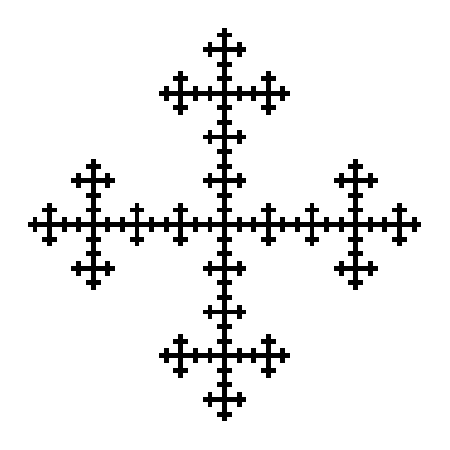
\begin{tikzpicture}[x=5cm,y=5cm]
      \fill (0.00000,0.49383) rectangle (0.01235,0.50617);
\fill (0.01235,0.50617) rectangle (0.02469,0.51852);
\fill (0.02469,0.49383) rectangle (0.03704,0.50617);
\fill (0.01235,0.48148) rectangle (0.02469,0.49383);
\fill (0.01235,0.49383) rectangle (0.02469,0.50617);
\fill (0.03704,0.53086) rectangle (0.04938,0.54321);
\fill (0.04938,0.54321) rectangle (0.06173,0.55556);
\fill (0.06173,0.53086) rectangle (0.07407,0.54321);
\fill (0.04938,0.51852) rectangle (0.06173,0.53086);
\fill (0.04938,0.53086) rectangle (0.06173,0.54321);
\fill (0.07407,0.49383) rectangle (0.08642,0.50617);
\fill (0.08642,0.50617) rectangle (0.09877,0.51852);
\fill (0.09877,0.49383) rectangle (0.11111,0.50617);
\fill (0.08642,0.48148) rectangle (0.09877,0.49383);
\fill (0.08642,0.49383) rectangle (0.09877,0.50617);
\fill (0.03704,0.45679) rectangle (0.04938,0.46914);
\fill (0.04938,0.46914) rectangle (0.06173,0.48148);
\fill (0.06173,0.45679) rectangle (0.07407,0.46914);
\fill (0.04938,0.44444) rectangle (0.06173,0.45679);
\fill (0.04938,0.45679) rectangle (0.06173,0.46914);
\fill (0.03704,0.49383) rectangle (0.04938,0.50617);
\fill (0.04938,0.50617) rectangle (0.06173,0.51852);
\fill (0.06173,0.49383) rectangle (0.07407,0.50617);
\fill (0.04938,0.48148) rectangle (0.06173,0.49383);
\fill (0.04938,0.49383) rectangle (0.06173,0.50617);
\fill (0.11111,0.60494) rectangle (0.12346,0.61728);
\fill (0.12346,0.61728) rectangle (0.13580,0.62963);
\fill (0.13580,0.60494) rectangle (0.14815,0.61728);
\fill (0.12346,0.59259) rectangle (0.13580,0.60494);
\fill (0.12346,0.60494) rectangle (0.13580,0.61728);
\fill (0.14815,0.64198) rectangle (0.16049,0.65432);
\fill (0.16049,0.65432) rectangle (0.17284,0.66667);
\fill (0.17284,0.64198) rectangle (0.18519,0.65432);
\fill (0.16049,0.62963) rectangle (0.17284,0.64198);
\fill (0.16049,0.64198) rectangle (0.17284,0.65432);
\fill (0.18519,0.60494) rectangle (0.19753,0.61728);
\fill (0.19753,0.61728) rectangle (0.20988,0.62963);
\fill (0.20988,0.60494) rectangle (0.22222,0.61728);
\fill (0.19753,0.59259) rectangle (0.20988,0.60494);
\fill (0.19753,0.60494) rectangle (0.20988,0.61728);
\fill (0.14815,0.56790) rectangle (0.16049,0.58025);
\fill (0.16049,0.58025) rectangle (0.17284,0.59259);
\fill (0.17284,0.56790) rectangle (0.18519,0.58025);
\fill (0.16049,0.55556) rectangle (0.17284,0.56790);
\fill (0.16049,0.56790) rectangle (0.17284,0.58025);
\fill (0.14815,0.60494) rectangle (0.16049,0.61728);
\fill (0.16049,0.61728) rectangle (0.17284,0.62963);
\fill (0.17284,0.60494) rectangle (0.18519,0.61728);
\fill (0.16049,0.59259) rectangle (0.17284,0.60494);
\fill (0.16049,0.60494) rectangle (0.17284,0.61728);
\fill (0.22222,0.49383) rectangle (0.23457,0.50617);
\fill (0.23457,0.50617) rectangle (0.24691,0.51852);
\fill (0.24691,0.49383) rectangle (0.25926,0.50617);
\fill (0.23457,0.48148) rectangle (0.24691,0.49383);
\fill (0.23457,0.49383) rectangle (0.24691,0.50617);
\fill (0.25926,0.53086) rectangle (0.27160,0.54321);
\fill (0.27160,0.54321) rectangle (0.28395,0.55556);
\fill (0.28395,0.53086) rectangle (0.29630,0.54321);
\fill (0.27160,0.51852) rectangle (0.28395,0.53086);
\fill (0.27160,0.53086) rectangle (0.28395,0.54321);
\fill (0.29630,0.49383) rectangle (0.30864,0.50617);
\fill (0.30864,0.50617) rectangle (0.32099,0.51852);
\fill (0.32099,0.49383) rectangle (0.33333,0.50617);
\fill (0.30864,0.48148) rectangle (0.32099,0.49383);
\fill (0.30864,0.49383) rectangle (0.32099,0.50617);
\fill (0.25926,0.45679) rectangle (0.27160,0.46914);
\fill (0.27160,0.46914) rectangle (0.28395,0.48148);
\fill (0.28395,0.45679) rectangle (0.29630,0.46914);
\fill (0.27160,0.44444) rectangle (0.28395,0.45679);
\fill (0.27160,0.45679) rectangle (0.28395,0.46914);
\fill (0.25926,0.49383) rectangle (0.27160,0.50617);
\fill (0.27160,0.50617) rectangle (0.28395,0.51852);
\fill (0.28395,0.49383) rectangle (0.29630,0.50617);
\fill (0.27160,0.48148) rectangle (0.28395,0.49383);
\fill (0.27160,0.49383) rectangle (0.28395,0.50617);
\fill (0.11111,0.38272) rectangle (0.12346,0.39506);
\fill (0.12346,0.39506) rectangle (0.13580,0.40741);
\fill (0.13580,0.38272) rectangle (0.14815,0.39506);
\fill (0.12346,0.37037) rectangle (0.13580,0.38272);
\fill (0.12346,0.38272) rectangle (0.13580,0.39506);
\fill (0.14815,0.41975) rectangle (0.16049,0.43210);
\fill (0.16049,0.43210) rectangle (0.17284,0.44444);
\fill (0.17284,0.41975) rectangle (0.18519,0.43210);
\fill (0.16049,0.40741) rectangle (0.17284,0.41975);
\fill (0.16049,0.41975) rectangle (0.17284,0.43210);
\fill (0.18519,0.38272) rectangle (0.19753,0.39506);
\fill (0.19753,0.39506) rectangle (0.20988,0.40741);
\fill (0.20988,0.38272) rectangle (0.22222,0.39506);
\fill (0.19753,0.37037) rectangle (0.20988,0.38272);
\fill (0.19753,0.38272) rectangle (0.20988,0.39506);
\fill (0.14815,0.34568) rectangle (0.16049,0.35802);
\fill (0.16049,0.35802) rectangle (0.17284,0.37037);
\fill (0.17284,0.34568) rectangle (0.18519,0.35802);
\fill (0.16049,0.33333) rectangle (0.17284,0.34568);
\fill (0.16049,0.34568) rectangle (0.17284,0.35802);
\fill (0.14815,0.38272) rectangle (0.16049,0.39506);
\fill (0.16049,0.39506) rectangle (0.17284,0.40741);
\fill (0.17284,0.38272) rectangle (0.18519,0.39506);
\fill (0.16049,0.37037) rectangle (0.17284,0.38272);
\fill (0.16049,0.38272) rectangle (0.17284,0.39506);
\fill (0.11111,0.49383) rectangle (0.12346,0.50617);
\fill (0.12346,0.50617) rectangle (0.13580,0.51852);
\fill (0.13580,0.49383) rectangle (0.14815,0.50617);
\fill (0.12346,0.48148) rectangle (0.13580,0.49383);
\fill (0.12346,0.49383) rectangle (0.13580,0.50617);
\fill (0.14815,0.53086) rectangle (0.16049,0.54321);
\fill (0.16049,0.54321) rectangle (0.17284,0.55556);
\fill (0.17284,0.53086) rectangle (0.18519,0.54321);
\fill (0.16049,0.51852) rectangle (0.17284,0.53086);
\fill (0.16049,0.53086) rectangle (0.17284,0.54321);
\fill (0.18519,0.49383) rectangle (0.19753,0.50617);
\fill (0.19753,0.50617) rectangle (0.20988,0.51852);
\fill (0.20988,0.49383) rectangle (0.22222,0.50617);
\fill (0.19753,0.48148) rectangle (0.20988,0.49383);
\fill (0.19753,0.49383) rectangle (0.20988,0.50617);
\fill (0.14815,0.45679) rectangle (0.16049,0.46914);
\fill (0.16049,0.46914) rectangle (0.17284,0.48148);
\fill (0.17284,0.45679) rectangle (0.18519,0.46914);
\fill (0.16049,0.44444) rectangle (0.17284,0.45679);
\fill (0.16049,0.45679) rectangle (0.17284,0.46914);
\fill (0.14815,0.49383) rectangle (0.16049,0.50617);
\fill (0.16049,0.50617) rectangle (0.17284,0.51852);
\fill (0.17284,0.49383) rectangle (0.18519,0.50617);
\fill (0.16049,0.48148) rectangle (0.17284,0.49383);
\fill (0.16049,0.49383) rectangle (0.17284,0.50617);
\fill (0.33333,0.82716) rectangle (0.34568,0.83951);
\fill (0.34568,0.83951) rectangle (0.35802,0.85185);
\fill (0.35802,0.82716) rectangle (0.37037,0.83951);
\fill (0.34568,0.81481) rectangle (0.35802,0.82716);
\fill (0.34568,0.82716) rectangle (0.35802,0.83951);
\fill (0.37037,0.86420) rectangle (0.38272,0.87654);
\fill (0.38272,0.87654) rectangle (0.39506,0.88889);
\fill (0.39506,0.86420) rectangle (0.40741,0.87654);
\fill (0.38272,0.85185) rectangle (0.39506,0.86420);
\fill (0.38272,0.86420) rectangle (0.39506,0.87654);
\fill (0.40741,0.82716) rectangle (0.41975,0.83951);
\fill (0.41975,0.83951) rectangle (0.43210,0.85185);
\fill (0.43210,0.82716) rectangle (0.44444,0.83951);
\fill (0.41975,0.81481) rectangle (0.43210,0.82716);
\fill (0.41975,0.82716) rectangle (0.43210,0.83951);
\fill (0.37037,0.79012) rectangle (0.38272,0.80247);
\fill (0.38272,0.80247) rectangle (0.39506,0.81481);
\fill (0.39506,0.79012) rectangle (0.40741,0.80247);
\fill (0.38272,0.77778) rectangle (0.39506,0.79012);
\fill (0.38272,0.79012) rectangle (0.39506,0.80247);
\fill (0.37037,0.82716) rectangle (0.38272,0.83951);
\fill (0.38272,0.83951) rectangle (0.39506,0.85185);
\fill (0.39506,0.82716) rectangle (0.40741,0.83951);
\fill (0.38272,0.81481) rectangle (0.39506,0.82716);
\fill (0.38272,0.82716) rectangle (0.39506,0.83951);
\fill (0.44444,0.93827) rectangle (0.45679,0.95062);
\fill (0.45679,0.95062) rectangle (0.46914,0.96296);
\fill (0.46914,0.93827) rectangle (0.48148,0.95062);
\fill (0.45679,0.92593) rectangle (0.46914,0.93827);
\fill (0.45679,0.93827) rectangle (0.46914,0.95062);
\fill (0.48148,0.97531) rectangle (0.49383,0.98765);
\fill (0.49383,0.98765) rectangle (0.50617,1.00000);
\fill (0.50617,0.97531) rectangle (0.51852,0.98765);
\fill (0.49383,0.96296) rectangle (0.50617,0.97531);
\fill (0.49383,0.97531) rectangle (0.50617,0.98765);
\fill (0.51852,0.93827) rectangle (0.53086,0.95062);
\fill (0.53086,0.95062) rectangle (0.54321,0.96296);
\fill (0.54321,0.93827) rectangle (0.55556,0.95062);
\fill (0.53086,0.92593) rectangle (0.54321,0.93827);
\fill (0.53086,0.93827) rectangle (0.54321,0.95062);
\fill (0.48148,0.90123) rectangle (0.49383,0.91358);
\fill (0.49383,0.91358) rectangle (0.50617,0.92593);
\fill (0.50617,0.90123) rectangle (0.51852,0.91358);
\fill (0.49383,0.88889) rectangle (0.50617,0.90123);
\fill (0.49383,0.90123) rectangle (0.50617,0.91358);
\fill (0.48148,0.93827) rectangle (0.49383,0.95062);
\fill (0.49383,0.95062) rectangle (0.50617,0.96296);
\fill (0.50617,0.93827) rectangle (0.51852,0.95062);
\fill (0.49383,0.92593) rectangle (0.50617,0.93827);
\fill (0.49383,0.93827) rectangle (0.50617,0.95062);
\fill (0.55556,0.82716) rectangle (0.56790,0.83951);
\fill (0.56790,0.83951) rectangle (0.58025,0.85185);
\fill (0.58025,0.82716) rectangle (0.59259,0.83951);
\fill (0.56790,0.81481) rectangle (0.58025,0.82716);
\fill (0.56790,0.82716) rectangle (0.58025,0.83951);
\fill (0.59259,0.86420) rectangle (0.60494,0.87654);
\fill (0.60494,0.87654) rectangle (0.61728,0.88889);
\fill (0.61728,0.86420) rectangle (0.62963,0.87654);
\fill (0.60494,0.85185) rectangle (0.61728,0.86420);
\fill (0.60494,0.86420) rectangle (0.61728,0.87654);
\fill (0.62963,0.82716) rectangle (0.64198,0.83951);
\fill (0.64198,0.83951) rectangle (0.65432,0.85185);
\fill (0.65432,0.82716) rectangle (0.66667,0.83951);
\fill (0.64198,0.81481) rectangle (0.65432,0.82716);
\fill (0.64198,0.82716) rectangle (0.65432,0.83951);
\fill (0.59259,0.79012) rectangle (0.60494,0.80247);
\fill (0.60494,0.80247) rectangle (0.61728,0.81481);
\fill (0.61728,0.79012) rectangle (0.62963,0.80247);
\fill (0.60494,0.77778) rectangle (0.61728,0.79012);
\fill (0.60494,0.79012) rectangle (0.61728,0.80247);
\fill (0.59259,0.82716) rectangle (0.60494,0.83951);
\fill (0.60494,0.83951) rectangle (0.61728,0.85185);
\fill (0.61728,0.82716) rectangle (0.62963,0.83951);
\fill (0.60494,0.81481) rectangle (0.61728,0.82716);
\fill (0.60494,0.82716) rectangle (0.61728,0.83951);
\fill (0.44444,0.71605) rectangle (0.45679,0.72840);
\fill (0.45679,0.72840) rectangle (0.46914,0.74074);
\fill (0.46914,0.71605) rectangle (0.48148,0.72840);
\fill (0.45679,0.70370) rectangle (0.46914,0.71605);
\fill (0.45679,0.71605) rectangle (0.46914,0.72840);
\fill (0.48148,0.75309) rectangle (0.49383,0.76543);
\fill (0.49383,0.76543) rectangle (0.50617,0.77778);
\fill (0.50617,0.75309) rectangle (0.51852,0.76543);
\fill (0.49383,0.74074) rectangle (0.50617,0.75309);
\fill (0.49383,0.75309) rectangle (0.50617,0.76543);
\fill (0.51852,0.71605) rectangle (0.53086,0.72840);
\fill (0.53086,0.72840) rectangle (0.54321,0.74074);
\fill (0.54321,0.71605) rectangle (0.55556,0.72840);
\fill (0.53086,0.70370) rectangle (0.54321,0.71605);
\fill (0.53086,0.71605) rectangle (0.54321,0.72840);
\fill (0.48148,0.67901) rectangle (0.49383,0.69136);
\fill (0.49383,0.69136) rectangle (0.50617,0.70370);
\fill (0.50617,0.67901) rectangle (0.51852,0.69136);
\fill (0.49383,0.66667) rectangle (0.50617,0.67901);
\fill (0.49383,0.67901) rectangle (0.50617,0.69136);
\fill (0.48148,0.71605) rectangle (0.49383,0.72840);
\fill (0.49383,0.72840) rectangle (0.50617,0.74074);
\fill (0.50617,0.71605) rectangle (0.51852,0.72840);
\fill (0.49383,0.70370) rectangle (0.50617,0.71605);
\fill (0.49383,0.71605) rectangle (0.50617,0.72840);
\fill (0.44444,0.82716) rectangle (0.45679,0.83951);
\fill (0.45679,0.83951) rectangle (0.46914,0.85185);
\fill (0.46914,0.82716) rectangle (0.48148,0.83951);
\fill (0.45679,0.81481) rectangle (0.46914,0.82716);
\fill (0.45679,0.82716) rectangle (0.46914,0.83951);
\fill (0.48148,0.86420) rectangle (0.49383,0.87654);
\fill (0.49383,0.87654) rectangle (0.50617,0.88889);
\fill (0.50617,0.86420) rectangle (0.51852,0.87654);
\fill (0.49383,0.85185) rectangle (0.50617,0.86420);
\fill (0.49383,0.86420) rectangle (0.50617,0.87654);
\fill (0.51852,0.82716) rectangle (0.53086,0.83951);
\fill (0.53086,0.83951) rectangle (0.54321,0.85185);
\fill (0.54321,0.82716) rectangle (0.55556,0.83951);
\fill (0.53086,0.81481) rectangle (0.54321,0.82716);
\fill (0.53086,0.82716) rectangle (0.54321,0.83951);
\fill (0.48148,0.79012) rectangle (0.49383,0.80247);
\fill (0.49383,0.80247) rectangle (0.50617,0.81481);
\fill (0.50617,0.79012) rectangle (0.51852,0.80247);
\fill (0.49383,0.77778) rectangle (0.50617,0.79012);
\fill (0.49383,0.79012) rectangle (0.50617,0.80247);
\fill (0.48148,0.82716) rectangle (0.49383,0.83951);
\fill (0.49383,0.83951) rectangle (0.50617,0.85185);
\fill (0.50617,0.82716) rectangle (0.51852,0.83951);
\fill (0.49383,0.81481) rectangle (0.50617,0.82716);
\fill (0.49383,0.82716) rectangle (0.50617,0.83951);
\fill (0.66667,0.49383) rectangle (0.67901,0.50617);
\fill (0.67901,0.50617) rectangle (0.69136,0.51852);
\fill (0.69136,0.49383) rectangle (0.70370,0.50617);
\fill (0.67901,0.48148) rectangle (0.69136,0.49383);
\fill (0.67901,0.49383) rectangle (0.69136,0.50617);
\fill (0.70370,0.53086) rectangle (0.71605,0.54321);
\fill (0.71605,0.54321) rectangle (0.72840,0.55556);
\fill (0.72840,0.53086) rectangle (0.74074,0.54321);
\fill (0.71605,0.51852) rectangle (0.72840,0.53086);
\fill (0.71605,0.53086) rectangle (0.72840,0.54321);
\fill (0.74074,0.49383) rectangle (0.75309,0.50617);
\fill (0.75309,0.50617) rectangle (0.76543,0.51852);
\fill (0.76543,0.49383) rectangle (0.77778,0.50617);
\fill (0.75309,0.48148) rectangle (0.76543,0.49383);
\fill (0.75309,0.49383) rectangle (0.76543,0.50617);
\fill (0.70370,0.45679) rectangle (0.71605,0.46914);
\fill (0.71605,0.46914) rectangle (0.72840,0.48148);
\fill (0.72840,0.45679) rectangle (0.74074,0.46914);
\fill (0.71605,0.44444) rectangle (0.72840,0.45679);
\fill (0.71605,0.45679) rectangle (0.72840,0.46914);
\fill (0.70370,0.49383) rectangle (0.71605,0.50617);
\fill (0.71605,0.50617) rectangle (0.72840,0.51852);
\fill (0.72840,0.49383) rectangle (0.74074,0.50617);
\fill (0.71605,0.48148) rectangle (0.72840,0.49383);
\fill (0.71605,0.49383) rectangle (0.72840,0.50617);
\fill (0.77778,0.60494) rectangle (0.79012,0.61728);
\fill (0.79012,0.61728) rectangle (0.80247,0.62963);
\fill (0.80247,0.60494) rectangle (0.81481,0.61728);
\fill (0.79012,0.59259) rectangle (0.80247,0.60494);
\fill (0.79012,0.60494) rectangle (0.80247,0.61728);
\fill (0.81481,0.64198) rectangle (0.82716,0.65432);
\fill (0.82716,0.65432) rectangle (0.83951,0.66667);
\fill (0.83951,0.64198) rectangle (0.85185,0.65432);
\fill (0.82716,0.62963) rectangle (0.83951,0.64198);
\fill (0.82716,0.64198) rectangle (0.83951,0.65432);
\fill (0.85185,0.60494) rectangle (0.86420,0.61728);
\fill (0.86420,0.61728) rectangle (0.87654,0.62963);
\fill (0.87654,0.60494) rectangle (0.88889,0.61728);
\fill (0.86420,0.59259) rectangle (0.87654,0.60494);
\fill (0.86420,0.60494) rectangle (0.87654,0.61728);
\fill (0.81481,0.56790) rectangle (0.82716,0.58025);
\fill (0.82716,0.58025) rectangle (0.83951,0.59259);
\fill (0.83951,0.56790) rectangle (0.85185,0.58025);
\fill (0.82716,0.55556) rectangle (0.83951,0.56790);
\fill (0.82716,0.56790) rectangle (0.83951,0.58025);
\fill (0.81481,0.60494) rectangle (0.82716,0.61728);
\fill (0.82716,0.61728) rectangle (0.83951,0.62963);
\fill (0.83951,0.60494) rectangle (0.85185,0.61728);
\fill (0.82716,0.59259) rectangle (0.83951,0.60494);
\fill (0.82716,0.60494) rectangle (0.83951,0.61728);
\fill (0.88889,0.49383) rectangle (0.90123,0.50617);
\fill (0.90123,0.50617) rectangle (0.91358,0.51852);
\fill (0.91358,0.49383) rectangle (0.92593,0.50617);
\fill (0.90123,0.48148) rectangle (0.91358,0.49383);
\fill (0.90123,0.49383) rectangle (0.91358,0.50617);
\fill (0.92593,0.53086) rectangle (0.93827,0.54321);
\fill (0.93827,0.54321) rectangle (0.95062,0.55556);
\fill (0.95062,0.53086) rectangle (0.96296,0.54321);
\fill (0.93827,0.51852) rectangle (0.95062,0.53086);
\fill (0.93827,0.53086) rectangle (0.95062,0.54321);
\fill (0.96296,0.49383) rectangle (0.97531,0.50617);
\fill (0.97531,0.50617) rectangle (0.98765,0.51852);
\fill (0.98765,0.49383) rectangle (1.00000,0.50617);
\fill (0.97531,0.48148) rectangle (0.98765,0.49383);
\fill (0.97531,0.49383) rectangle (0.98765,0.50617);
\fill (0.92593,0.45679) rectangle (0.93827,0.46914);
\fill (0.93827,0.46914) rectangle (0.95062,0.48148);
\fill (0.95062,0.45679) rectangle (0.96296,0.46914);
\fill (0.93827,0.44444) rectangle (0.95062,0.45679);
\fill (0.93827,0.45679) rectangle (0.95062,0.46914);
\fill (0.92593,0.49383) rectangle (0.93827,0.50617);
\fill (0.93827,0.50617) rectangle (0.95062,0.51852);
\fill (0.95062,0.49383) rectangle (0.96296,0.50617);
\fill (0.93827,0.48148) rectangle (0.95062,0.49383);
\fill (0.93827,0.49383) rectangle (0.95062,0.50617);
\fill (0.77778,0.38272) rectangle (0.79012,0.39506);
\fill (0.79012,0.39506) rectangle (0.80247,0.40741);
\fill (0.80247,0.38272) rectangle (0.81481,0.39506);
\fill (0.79012,0.37037) rectangle (0.80247,0.38272);
\fill (0.79012,0.38272) rectangle (0.80247,0.39506);
\fill (0.81481,0.41975) rectangle (0.82716,0.43210);
\fill (0.82716,0.43210) rectangle (0.83951,0.44444);
\fill (0.83951,0.41975) rectangle (0.85185,0.43210);
\fill (0.82716,0.40741) rectangle (0.83951,0.41975);
\fill (0.82716,0.41975) rectangle (0.83951,0.43210);
\fill (0.85185,0.38272) rectangle (0.86420,0.39506);
\fill (0.86420,0.39506) rectangle (0.87654,0.40741);
\fill (0.87654,0.38272) rectangle (0.88889,0.39506);
\fill (0.86420,0.37037) rectangle (0.87654,0.38272);
\fill (0.86420,0.38272) rectangle (0.87654,0.39506);
\fill (0.81481,0.34568) rectangle (0.82716,0.35802);
\fill (0.82716,0.35802) rectangle (0.83951,0.37037);
\fill (0.83951,0.34568) rectangle (0.85185,0.35802);
\fill (0.82716,0.33333) rectangle (0.83951,0.34568);
\fill (0.82716,0.34568) rectangle (0.83951,0.35802);
\fill (0.81481,0.38272) rectangle (0.82716,0.39506);
\fill (0.82716,0.39506) rectangle (0.83951,0.40741);
\fill (0.83951,0.38272) rectangle (0.85185,0.39506);
\fill (0.82716,0.37037) rectangle (0.83951,0.38272);
\fill (0.82716,0.38272) rectangle (0.83951,0.39506);
\fill (0.77778,0.49383) rectangle (0.79012,0.50617);
\fill (0.79012,0.50617) rectangle (0.80247,0.51852);
\fill (0.80247,0.49383) rectangle (0.81481,0.50617);
\fill (0.79012,0.48148) rectangle (0.80247,0.49383);
\fill (0.79012,0.49383) rectangle (0.80247,0.50617);
\fill (0.81481,0.53086) rectangle (0.82716,0.54321);
\fill (0.82716,0.54321) rectangle (0.83951,0.55556);
\fill (0.83951,0.53086) rectangle (0.85185,0.54321);
\fill (0.82716,0.51852) rectangle (0.83951,0.53086);
\fill (0.82716,0.53086) rectangle (0.83951,0.54321);
\fill (0.85185,0.49383) rectangle (0.86420,0.50617);
\fill (0.86420,0.50617) rectangle (0.87654,0.51852);
\fill (0.87654,0.49383) rectangle (0.88889,0.50617);
\fill (0.86420,0.48148) rectangle (0.87654,0.49383);
\fill (0.86420,0.49383) rectangle (0.87654,0.50617);
\fill (0.81481,0.45679) rectangle (0.82716,0.46914);
\fill (0.82716,0.46914) rectangle (0.83951,0.48148);
\fill (0.83951,0.45679) rectangle (0.85185,0.46914);
\fill (0.82716,0.44444) rectangle (0.83951,0.45679);
\fill (0.82716,0.45679) rectangle (0.83951,0.46914);
\fill (0.81481,0.49383) rectangle (0.82716,0.50617);
\fill (0.82716,0.50617) rectangle (0.83951,0.51852);
\fill (0.83951,0.49383) rectangle (0.85185,0.50617);
\fill (0.82716,0.48148) rectangle (0.83951,0.49383);
\fill (0.82716,0.49383) rectangle (0.83951,0.50617);
\fill (0.33333,0.16049) rectangle (0.34568,0.17284);
\fill (0.34568,0.17284) rectangle (0.35802,0.18519);
\fill (0.35802,0.16049) rectangle (0.37037,0.17284);
\fill (0.34568,0.14815) rectangle (0.35802,0.16049);
\fill (0.34568,0.16049) rectangle (0.35802,0.17284);
\fill (0.37037,0.19753) rectangle (0.38272,0.20988);
\fill (0.38272,0.20988) rectangle (0.39506,0.22222);
\fill (0.39506,0.19753) rectangle (0.40741,0.20988);
\fill (0.38272,0.18519) rectangle (0.39506,0.19753);
\fill (0.38272,0.19753) rectangle (0.39506,0.20988);
\fill (0.40741,0.16049) rectangle (0.41975,0.17284);
\fill (0.41975,0.17284) rectangle (0.43210,0.18519);
\fill (0.43210,0.16049) rectangle (0.44444,0.17284);
\fill (0.41975,0.14815) rectangle (0.43210,0.16049);
\fill (0.41975,0.16049) rectangle (0.43210,0.17284);
\fill (0.37037,0.12346) rectangle (0.38272,0.13580);
\fill (0.38272,0.13580) rectangle (0.39506,0.14815);
\fill (0.39506,0.12346) rectangle (0.40741,0.13580);
\fill (0.38272,0.11111) rectangle (0.39506,0.12346);
\fill (0.38272,0.12346) rectangle (0.39506,0.13580);
\fill (0.37037,0.16049) rectangle (0.38272,0.17284);
\fill (0.38272,0.17284) rectangle (0.39506,0.18519);
\fill (0.39506,0.16049) rectangle (0.40741,0.17284);
\fill (0.38272,0.14815) rectangle (0.39506,0.16049);
\fill (0.38272,0.16049) rectangle (0.39506,0.17284);
\fill (0.44444,0.27160) rectangle (0.45679,0.28395);
\fill (0.45679,0.28395) rectangle (0.46914,0.29630);
\fill (0.46914,0.27160) rectangle (0.48148,0.28395);
\fill (0.45679,0.25926) rectangle (0.46914,0.27160);
\fill (0.45679,0.27160) rectangle (0.46914,0.28395);
\fill (0.48148,0.30864) rectangle (0.49383,0.32099);
\fill (0.49383,0.32099) rectangle (0.50617,0.33333);
\fill (0.50617,0.30864) rectangle (0.51852,0.32099);
\fill (0.49383,0.29630) rectangle (0.50617,0.30864);
\fill (0.49383,0.30864) rectangle (0.50617,0.32099);
\fill (0.51852,0.27160) rectangle (0.53086,0.28395);
\fill (0.53086,0.28395) rectangle (0.54321,0.29630);
\fill (0.54321,0.27160) rectangle (0.55556,0.28395);
\fill (0.53086,0.25926) rectangle (0.54321,0.27160);
\fill (0.53086,0.27160) rectangle (0.54321,0.28395);
\fill (0.48148,0.23457) rectangle (0.49383,0.24691);
\fill (0.49383,0.24691) rectangle (0.50617,0.25926);
\fill (0.50617,0.23457) rectangle (0.51852,0.24691);
\fill (0.49383,0.22222) rectangle (0.50617,0.23457);
\fill (0.49383,0.23457) rectangle (0.50617,0.24691);
\fill (0.48148,0.27160) rectangle (0.49383,0.28395);
\fill (0.49383,0.28395) rectangle (0.50617,0.29630);
\fill (0.50617,0.27160) rectangle (0.51852,0.28395);
\fill (0.49383,0.25926) rectangle (0.50617,0.27160);
\fill (0.49383,0.27160) rectangle (0.50617,0.28395);
\fill (0.55556,0.16049) rectangle (0.56790,0.17284);
\fill (0.56790,0.17284) rectangle (0.58025,0.18519);
\fill (0.58025,0.16049) rectangle (0.59259,0.17284);
\fill (0.56790,0.14815) rectangle (0.58025,0.16049);
\fill (0.56790,0.16049) rectangle (0.58025,0.17284);
\fill (0.59259,0.19753) rectangle (0.60494,0.20988);
\fill (0.60494,0.20988) rectangle (0.61728,0.22222);
\fill (0.61728,0.19753) rectangle (0.62963,0.20988);
\fill (0.60494,0.18519) rectangle (0.61728,0.19753);
\fill (0.60494,0.19753) rectangle (0.61728,0.20988);
\fill (0.62963,0.16049) rectangle (0.64198,0.17284);
\fill (0.64198,0.17284) rectangle (0.65432,0.18519);
\fill (0.65432,0.16049) rectangle (0.66667,0.17284);
\fill (0.64198,0.14815) rectangle (0.65432,0.16049);
\fill (0.64198,0.16049) rectangle (0.65432,0.17284);
\fill (0.59259,0.12346) rectangle (0.60494,0.13580);
\fill (0.60494,0.13580) rectangle (0.61728,0.14815);
\fill (0.61728,0.12346) rectangle (0.62963,0.13580);
\fill (0.60494,0.11111) rectangle (0.61728,0.12346);
\fill (0.60494,0.12346) rectangle (0.61728,0.13580);
\fill (0.59259,0.16049) rectangle (0.60494,0.17284);
\fill (0.60494,0.17284) rectangle (0.61728,0.18519);
\fill (0.61728,0.16049) rectangle (0.62963,0.17284);
\fill (0.60494,0.14815) rectangle (0.61728,0.16049);
\fill (0.60494,0.16049) rectangle (0.61728,0.17284);
\fill (0.44444,0.04938) rectangle (0.45679,0.06173);
\fill (0.45679,0.06173) rectangle (0.46914,0.07407);
\fill (0.46914,0.04938) rectangle (0.48148,0.06173);
\fill (0.45679,0.03704) rectangle (0.46914,0.04938);
\fill (0.45679,0.04938) rectangle (0.46914,0.06173);
\fill (0.48148,0.08642) rectangle (0.49383,0.09877);
\fill (0.49383,0.09877) rectangle (0.50617,0.11111);
\fill (0.50617,0.08642) rectangle (0.51852,0.09877);
\fill (0.49383,0.07407) rectangle (0.50617,0.08642);
\fill (0.49383,0.08642) rectangle (0.50617,0.09877);
\fill (0.51852,0.04938) rectangle (0.53086,0.06173);
\fill (0.53086,0.06173) rectangle (0.54321,0.07407);
\fill (0.54321,0.04938) rectangle (0.55556,0.06173);
\fill (0.53086,0.03704) rectangle (0.54321,0.04938);
\fill (0.53086,0.04938) rectangle (0.54321,0.06173);
\fill (0.48148,0.01235) rectangle (0.49383,0.02469);
\fill (0.49383,0.02469) rectangle (0.50617,0.03704);
\fill (0.50617,0.01235) rectangle (0.51852,0.02469);
\fill (0.49383,0.00000) rectangle (0.50617,0.01235);
\fill (0.49383,0.01235) rectangle (0.50617,0.02469);
\fill (0.48148,0.04938) rectangle (0.49383,0.06173);
\fill (0.49383,0.06173) rectangle (0.50617,0.07407);
\fill (0.50617,0.04938) rectangle (0.51852,0.06173);
\fill (0.49383,0.03704) rectangle (0.50617,0.04938);
\fill (0.49383,0.04938) rectangle (0.50617,0.06173);
\fill (0.44444,0.16049) rectangle (0.45679,0.17284);
\fill (0.45679,0.17284) rectangle (0.46914,0.18519);
\fill (0.46914,0.16049) rectangle (0.48148,0.17284);
\fill (0.45679,0.14815) rectangle (0.46914,0.16049);
\fill (0.45679,0.16049) rectangle (0.46914,0.17284);
\fill (0.48148,0.19753) rectangle (0.49383,0.20988);
\fill (0.49383,0.20988) rectangle (0.50617,0.22222);
\fill (0.50617,0.19753) rectangle (0.51852,0.20988);
\fill (0.49383,0.18519) rectangle (0.50617,0.19753);
\fill (0.49383,0.19753) rectangle (0.50617,0.20988);
\fill (0.51852,0.16049) rectangle (0.53086,0.17284);
\fill (0.53086,0.17284) rectangle (0.54321,0.18519);
\fill (0.54321,0.16049) rectangle (0.55556,0.17284);
\fill (0.53086,0.14815) rectangle (0.54321,0.16049);
\fill (0.53086,0.16049) rectangle (0.54321,0.17284);
\fill (0.48148,0.12346) rectangle (0.49383,0.13580);
\fill (0.49383,0.13580) rectangle (0.50617,0.14815);
\fill (0.50617,0.12346) rectangle (0.51852,0.13580);
\fill (0.49383,0.11111) rectangle (0.50617,0.12346);
\fill (0.49383,0.12346) rectangle (0.50617,0.13580);
\fill (0.48148,0.16049) rectangle (0.49383,0.17284);
\fill (0.49383,0.17284) rectangle (0.50617,0.18519);
\fill (0.50617,0.16049) rectangle (0.51852,0.17284);
\fill (0.49383,0.14815) rectangle (0.50617,0.16049);
\fill (0.49383,0.16049) rectangle (0.50617,0.17284);
\fill (0.33333,0.49383) rectangle (0.34568,0.50617);
\fill (0.34568,0.50617) rectangle (0.35802,0.51852);
\fill (0.35802,0.49383) rectangle (0.37037,0.50617);
\fill (0.34568,0.48148) rectangle (0.35802,0.49383);
\fill (0.34568,0.49383) rectangle (0.35802,0.50617);
\fill (0.37037,0.53086) rectangle (0.38272,0.54321);
\fill (0.38272,0.54321) rectangle (0.39506,0.55556);
\fill (0.39506,0.53086) rectangle (0.40741,0.54321);
\fill (0.38272,0.51852) rectangle (0.39506,0.53086);
\fill (0.38272,0.53086) rectangle (0.39506,0.54321);
\fill (0.40741,0.49383) rectangle (0.41975,0.50617);
\fill (0.41975,0.50617) rectangle (0.43210,0.51852);
\fill (0.43210,0.49383) rectangle (0.44444,0.50617);
\fill (0.41975,0.48148) rectangle (0.43210,0.49383);
\fill (0.41975,0.49383) rectangle (0.43210,0.50617);
\fill (0.37037,0.45679) rectangle (0.38272,0.46914);
\fill (0.38272,0.46914) rectangle (0.39506,0.48148);
\fill (0.39506,0.45679) rectangle (0.40741,0.46914);
\fill (0.38272,0.44444) rectangle (0.39506,0.45679);
\fill (0.38272,0.45679) rectangle (0.39506,0.46914);
\fill (0.37037,0.49383) rectangle (0.38272,0.50617);
\fill (0.38272,0.50617) rectangle (0.39506,0.51852);
\fill (0.39506,0.49383) rectangle (0.40741,0.50617);
\fill (0.38272,0.48148) rectangle (0.39506,0.49383);
\fill (0.38272,0.49383) rectangle (0.39506,0.50617);
\fill (0.44444,0.60494) rectangle (0.45679,0.61728);
\fill (0.45679,0.61728) rectangle (0.46914,0.62963);
\fill (0.46914,0.60494) rectangle (0.48148,0.61728);
\fill (0.45679,0.59259) rectangle (0.46914,0.60494);
\fill (0.45679,0.60494) rectangle (0.46914,0.61728);
\fill (0.48148,0.64198) rectangle (0.49383,0.65432);
\fill (0.49383,0.65432) rectangle (0.50617,0.66667);
\fill (0.50617,0.64198) rectangle (0.51852,0.65432);
\fill (0.49383,0.62963) rectangle (0.50617,0.64198);
\fill (0.49383,0.64198) rectangle (0.50617,0.65432);
\fill (0.51852,0.60494) rectangle (0.53086,0.61728);
\fill (0.53086,0.61728) rectangle (0.54321,0.62963);
\fill (0.54321,0.60494) rectangle (0.55556,0.61728);
\fill (0.53086,0.59259) rectangle (0.54321,0.60494);
\fill (0.53086,0.60494) rectangle (0.54321,0.61728);
\fill (0.48148,0.56790) rectangle (0.49383,0.58025);
\fill (0.49383,0.58025) rectangle (0.50617,0.59259);
\fill (0.50617,0.56790) rectangle (0.51852,0.58025);
\fill (0.49383,0.55556) rectangle (0.50617,0.56790);
\fill (0.49383,0.56790) rectangle (0.50617,0.58025);
\fill (0.48148,0.60494) rectangle (0.49383,0.61728);
\fill (0.49383,0.61728) rectangle (0.50617,0.62963);
\fill (0.50617,0.60494) rectangle (0.51852,0.61728);
\fill (0.49383,0.59259) rectangle (0.50617,0.60494);
\fill (0.49383,0.60494) rectangle (0.50617,0.61728);
\fill (0.55556,0.49383) rectangle (0.56790,0.50617);
\fill (0.56790,0.50617) rectangle (0.58025,0.51852);
\fill (0.58025,0.49383) rectangle (0.59259,0.50617);
\fill (0.56790,0.48148) rectangle (0.58025,0.49383);
\fill (0.56790,0.49383) rectangle (0.58025,0.50617);
\fill (0.59259,0.53086) rectangle (0.60494,0.54321);
\fill (0.60494,0.54321) rectangle (0.61728,0.55556);
\fill (0.61728,0.53086) rectangle (0.62963,0.54321);
\fill (0.60494,0.51852) rectangle (0.61728,0.53086);
\fill (0.60494,0.53086) rectangle (0.61728,0.54321);
\fill (0.62963,0.49383) rectangle (0.64198,0.50617);
\fill (0.64198,0.50617) rectangle (0.65432,0.51852);
\fill (0.65432,0.49383) rectangle (0.66667,0.50617);
\fill (0.64198,0.48148) rectangle (0.65432,0.49383);
\fill (0.64198,0.49383) rectangle (0.65432,0.50617);
\fill (0.59259,0.45679) rectangle (0.60494,0.46914);
\fill (0.60494,0.46914) rectangle (0.61728,0.48148);
\fill (0.61728,0.45679) rectangle (0.62963,0.46914);
\fill (0.60494,0.44444) rectangle (0.61728,0.45679);
\fill (0.60494,0.45679) rectangle (0.61728,0.46914);
\fill (0.59259,0.49383) rectangle (0.60494,0.50617);
\fill (0.60494,0.50617) rectangle (0.61728,0.51852);
\fill (0.61728,0.49383) rectangle (0.62963,0.50617);
\fill (0.60494,0.48148) rectangle (0.61728,0.49383);
\fill (0.60494,0.49383) rectangle (0.61728,0.50617);
\fill (0.44444,0.38272) rectangle (0.45679,0.39506);
\fill (0.45679,0.39506) rectangle (0.46914,0.40741);
\fill (0.46914,0.38272) rectangle (0.48148,0.39506);
\fill (0.45679,0.37037) rectangle (0.46914,0.38272);
\fill (0.45679,0.38272) rectangle (0.46914,0.39506);
\fill (0.48148,0.41975) rectangle (0.49383,0.43210);
\fill (0.49383,0.43210) rectangle (0.50617,0.44444);
\fill (0.50617,0.41975) rectangle (0.51852,0.43210);
\fill (0.49383,0.40741) rectangle (0.50617,0.41975);
\fill (0.49383,0.41975) rectangle (0.50617,0.43210);
\fill (0.51852,0.38272) rectangle (0.53086,0.39506);
\fill (0.53086,0.39506) rectangle (0.54321,0.40741);
\fill (0.54321,0.38272) rectangle (0.55556,0.39506);
\fill (0.53086,0.37037) rectangle (0.54321,0.38272);
\fill (0.53086,0.38272) rectangle (0.54321,0.39506);
\fill (0.48148,0.34568) rectangle (0.49383,0.35802);
\fill (0.49383,0.35802) rectangle (0.50617,0.37037);
\fill (0.50617,0.34568) rectangle (0.51852,0.35802);
\fill (0.49383,0.33333) rectangle (0.50617,0.34568);
\fill (0.49383,0.34568) rectangle (0.50617,0.35802);
\fill (0.48148,0.38272) rectangle (0.49383,0.39506);
\fill (0.49383,0.39506) rectangle (0.50617,0.40741);
\fill (0.50617,0.38272) rectangle (0.51852,0.39506);
\fill (0.49383,0.37037) rectangle (0.50617,0.38272);
\fill (0.49383,0.38272) rectangle (0.50617,0.39506);
\fill (0.44444,0.49383) rectangle (0.45679,0.50617);
\fill (0.45679,0.50617) rectangle (0.46914,0.51852);
\fill (0.46914,0.49383) rectangle (0.48148,0.50617);
\fill (0.45679,0.48148) rectangle (0.46914,0.49383);
\fill (0.45679,0.49383) rectangle (0.46914,0.50617);
\fill (0.48148,0.53086) rectangle (0.49383,0.54321);
\fill (0.49383,0.54321) rectangle (0.50617,0.55556);
\fill (0.50617,0.53086) rectangle (0.51852,0.54321);
\fill (0.49383,0.51852) rectangle (0.50617,0.53086);
\fill (0.49383,0.53086) rectangle (0.50617,0.54321);
\fill (0.51852,0.49383) rectangle (0.53086,0.50617);
\fill (0.53086,0.50617) rectangle (0.54321,0.51852);
\fill (0.54321,0.49383) rectangle (0.55556,0.50617);
\fill (0.53086,0.48148) rectangle (0.54321,0.49383);
\fill (0.53086,0.49383) rectangle (0.54321,0.50617);
\fill (0.48148,0.45679) rectangle (0.49383,0.46914);
\fill (0.49383,0.46914) rectangle (0.50617,0.48148);
\fill (0.50617,0.45679) rectangle (0.51852,0.46914);
\fill (0.49383,0.44444) rectangle (0.50617,0.45679);
\fill (0.49383,0.45679) rectangle (0.50617,0.46914);
\fill (0.48148,0.49383) rectangle (0.49383,0.50617);
\fill (0.49383,0.50617) rectangle (0.50617,0.51852);
\fill (0.50617,0.49383) rectangle (0.51852,0.50617);
\fill (0.49383,0.48148) rectangle (0.50617,0.49383);
\fill (0.49383,0.49383) rectangle (0.50617,0.50617);

    \end{tikzpicture}
    \caption{Vicsek fractal}
  \end{subfigure}
  \hfill
  \begin{subfigure}[b]{0.45\textwidth}
    \centering
    
\begin{tikzpicture}[x=5cm,y=5cm]
      \fill (0.00000,0.48148) rectangle (0.03704,0.51852);
\fill (0.03704,0.51852) rectangle (0.07407,0.55556);
\fill (0.07407,0.48148) rectangle (0.11111,0.51852);
\fill (0.00000,0.44444) rectangle (0.03704,0.48148);
\fill (0.07407,0.44444) rectangle (0.11111,0.48148);
\fill (0.00000,0.51852) rectangle (0.03704,0.55556);
\fill (0.07407,0.51852) rectangle (0.11111,0.55556);
\fill (0.03704,0.44444) rectangle (0.07407,0.48148);
\fill (0.11111,0.59259) rectangle (0.14815,0.62963);
\fill (0.14815,0.62963) rectangle (0.18519,0.66667);
\fill (0.18519,0.59259) rectangle (0.22222,0.62963);
\fill (0.11111,0.55556) rectangle (0.14815,0.59259);
\fill (0.18519,0.55556) rectangle (0.22222,0.59259);
\fill (0.11111,0.62963) rectangle (0.14815,0.66667);
\fill (0.18519,0.62963) rectangle (0.22222,0.66667);
\fill (0.14815,0.55556) rectangle (0.18519,0.59259);
\fill (0.22222,0.48148) rectangle (0.25926,0.51852);
\fill (0.25926,0.51852) rectangle (0.29630,0.55556);
\fill (0.29630,0.48148) rectangle (0.33333,0.51852);
\fill (0.22222,0.44444) rectangle (0.25926,0.48148);
\fill (0.29630,0.44444) rectangle (0.33333,0.48148);
\fill (0.22222,0.51852) rectangle (0.25926,0.55556);
\fill (0.29630,0.51852) rectangle (0.33333,0.55556);
\fill (0.25926,0.44444) rectangle (0.29630,0.48148);
\fill (0.00000,0.37037) rectangle (0.03704,0.40741);
\fill (0.03704,0.40741) rectangle (0.07407,0.44444);
\fill (0.07407,0.37037) rectangle (0.11111,0.40741);
\fill (0.00000,0.33333) rectangle (0.03704,0.37037);
\fill (0.07407,0.33333) rectangle (0.11111,0.37037);
\fill (0.00000,0.40741) rectangle (0.03704,0.44444);
\fill (0.07407,0.40741) rectangle (0.11111,0.44444);
\fill (0.03704,0.33333) rectangle (0.07407,0.37037);
\fill (0.22222,0.37037) rectangle (0.25926,0.40741);
\fill (0.25926,0.40741) rectangle (0.29630,0.44444);
\fill (0.29630,0.37037) rectangle (0.33333,0.40741);
\fill (0.22222,0.33333) rectangle (0.25926,0.37037);
\fill (0.29630,0.33333) rectangle (0.33333,0.37037);
\fill (0.22222,0.40741) rectangle (0.25926,0.44444);
\fill (0.29630,0.40741) rectangle (0.33333,0.44444);
\fill (0.25926,0.33333) rectangle (0.29630,0.37037);
\fill (0.00000,0.59259) rectangle (0.03704,0.62963);
\fill (0.03704,0.62963) rectangle (0.07407,0.66667);
\fill (0.07407,0.59259) rectangle (0.11111,0.62963);
\fill (0.00000,0.55556) rectangle (0.03704,0.59259);
\fill (0.07407,0.55556) rectangle (0.11111,0.59259);
\fill (0.00000,0.62963) rectangle (0.03704,0.66667);
\fill (0.07407,0.62963) rectangle (0.11111,0.66667);
\fill (0.03704,0.55556) rectangle (0.07407,0.59259);
\fill (0.22222,0.59259) rectangle (0.25926,0.62963);
\fill (0.25926,0.62963) rectangle (0.29630,0.66667);
\fill (0.29630,0.59259) rectangle (0.33333,0.62963);
\fill (0.22222,0.55556) rectangle (0.25926,0.59259);
\fill (0.29630,0.55556) rectangle (0.33333,0.59259);
\fill (0.22222,0.62963) rectangle (0.25926,0.66667);
\fill (0.29630,0.62963) rectangle (0.33333,0.66667);
\fill (0.25926,0.55556) rectangle (0.29630,0.59259);
\fill (0.11111,0.37037) rectangle (0.14815,0.40741);
\fill (0.14815,0.40741) rectangle (0.18519,0.44444);
\fill (0.18519,0.37037) rectangle (0.22222,0.40741);
\fill (0.11111,0.33333) rectangle (0.14815,0.37037);
\fill (0.18519,0.33333) rectangle (0.22222,0.37037);
\fill (0.11111,0.40741) rectangle (0.14815,0.44444);
\fill (0.18519,0.40741) rectangle (0.22222,0.44444);
\fill (0.14815,0.33333) rectangle (0.18519,0.37037);
\fill (0.33333,0.81481) rectangle (0.37037,0.85185);
\fill (0.37037,0.85185) rectangle (0.40741,0.88889);
\fill (0.40741,0.81481) rectangle (0.44444,0.85185);
\fill (0.33333,0.77778) rectangle (0.37037,0.81481);
\fill (0.40741,0.77778) rectangle (0.44444,0.81481);
\fill (0.33333,0.85185) rectangle (0.37037,0.88889);
\fill (0.40741,0.85185) rectangle (0.44444,0.88889);
\fill (0.37037,0.77778) rectangle (0.40741,0.81481);
\fill (0.44444,0.92593) rectangle (0.48148,0.96296);
\fill (0.48148,0.96296) rectangle (0.51852,1.00000);
\fill (0.51852,0.92593) rectangle (0.55556,0.96296);
\fill (0.44444,0.88889) rectangle (0.48148,0.92593);
\fill (0.51852,0.88889) rectangle (0.55556,0.92593);
\fill (0.44444,0.96296) rectangle (0.48148,1.00000);
\fill (0.51852,0.96296) rectangle (0.55556,1.00000);
\fill (0.48148,0.88889) rectangle (0.51852,0.92593);
\fill (0.55556,0.81481) rectangle (0.59259,0.85185);
\fill (0.59259,0.85185) rectangle (0.62963,0.88889);
\fill (0.62963,0.81481) rectangle (0.66667,0.85185);
\fill (0.55556,0.77778) rectangle (0.59259,0.81481);
\fill (0.62963,0.77778) rectangle (0.66667,0.81481);
\fill (0.55556,0.85185) rectangle (0.59259,0.88889);
\fill (0.62963,0.85185) rectangle (0.66667,0.88889);
\fill (0.59259,0.77778) rectangle (0.62963,0.81481);
\fill (0.33333,0.70370) rectangle (0.37037,0.74074);
\fill (0.37037,0.74074) rectangle (0.40741,0.77778);
\fill (0.40741,0.70370) rectangle (0.44444,0.74074);
\fill (0.33333,0.66667) rectangle (0.37037,0.70370);
\fill (0.40741,0.66667) rectangle (0.44444,0.70370);
\fill (0.33333,0.74074) rectangle (0.37037,0.77778);
\fill (0.40741,0.74074) rectangle (0.44444,0.77778);
\fill (0.37037,0.66667) rectangle (0.40741,0.70370);
\fill (0.55556,0.70370) rectangle (0.59259,0.74074);
\fill (0.59259,0.74074) rectangle (0.62963,0.77778);
\fill (0.62963,0.70370) rectangle (0.66667,0.74074);
\fill (0.55556,0.66667) rectangle (0.59259,0.70370);
\fill (0.62963,0.66667) rectangle (0.66667,0.70370);
\fill (0.55556,0.74074) rectangle (0.59259,0.77778);
\fill (0.62963,0.74074) rectangle (0.66667,0.77778);
\fill (0.59259,0.66667) rectangle (0.62963,0.70370);
\fill (0.33333,0.92593) rectangle (0.37037,0.96296);
\fill (0.37037,0.96296) rectangle (0.40741,1.00000);
\fill (0.40741,0.92593) rectangle (0.44444,0.96296);
\fill (0.33333,0.88889) rectangle (0.37037,0.92593);
\fill (0.40741,0.88889) rectangle (0.44444,0.92593);
\fill (0.33333,0.96296) rectangle (0.37037,1.00000);
\fill (0.40741,0.96296) rectangle (0.44444,1.00000);
\fill (0.37037,0.88889) rectangle (0.40741,0.92593);
\fill (0.55556,0.92593) rectangle (0.59259,0.96296);
\fill (0.59259,0.96296) rectangle (0.62963,1.00000);
\fill (0.62963,0.92593) rectangle (0.66667,0.96296);
\fill (0.55556,0.88889) rectangle (0.59259,0.92593);
\fill (0.62963,0.88889) rectangle (0.66667,0.92593);
\fill (0.55556,0.96296) rectangle (0.59259,1.00000);
\fill (0.62963,0.96296) rectangle (0.66667,1.00000);
\fill (0.59259,0.88889) rectangle (0.62963,0.92593);
\fill (0.44444,0.70370) rectangle (0.48148,0.74074);
\fill (0.48148,0.74074) rectangle (0.51852,0.77778);
\fill (0.51852,0.70370) rectangle (0.55556,0.74074);
\fill (0.44444,0.66667) rectangle (0.48148,0.70370);
\fill (0.51852,0.66667) rectangle (0.55556,0.70370);
\fill (0.44444,0.74074) rectangle (0.48148,0.77778);
\fill (0.51852,0.74074) rectangle (0.55556,0.77778);
\fill (0.48148,0.66667) rectangle (0.51852,0.70370);
\fill (0.66667,0.48148) rectangle (0.70370,0.51852);
\fill (0.70370,0.51852) rectangle (0.74074,0.55556);
\fill (0.74074,0.48148) rectangle (0.77778,0.51852);
\fill (0.66667,0.44444) rectangle (0.70370,0.48148);
\fill (0.74074,0.44444) rectangle (0.77778,0.48148);
\fill (0.66667,0.51852) rectangle (0.70370,0.55556);
\fill (0.74074,0.51852) rectangle (0.77778,0.55556);
\fill (0.70370,0.44444) rectangle (0.74074,0.48148);
\fill (0.77778,0.59259) rectangle (0.81481,0.62963);
\fill (0.81481,0.62963) rectangle (0.85185,0.66667);
\fill (0.85185,0.59259) rectangle (0.88889,0.62963);
\fill (0.77778,0.55556) rectangle (0.81481,0.59259);
\fill (0.85185,0.55556) rectangle (0.88889,0.59259);
\fill (0.77778,0.62963) rectangle (0.81481,0.66667);
\fill (0.85185,0.62963) rectangle (0.88889,0.66667);
\fill (0.81481,0.55556) rectangle (0.85185,0.59259);
\fill (0.88889,0.48148) rectangle (0.92593,0.51852);
\fill (0.92593,0.51852) rectangle (0.96296,0.55556);
\fill (0.96296,0.48148) rectangle (1.00000,0.51852);
\fill (0.88889,0.44444) rectangle (0.92593,0.48148);
\fill (0.96296,0.44444) rectangle (1.00000,0.48148);
\fill (0.88889,0.51852) rectangle (0.92593,0.55556);
\fill (0.96296,0.51852) rectangle (1.00000,0.55556);
\fill (0.92593,0.44444) rectangle (0.96296,0.48148);
\fill (0.66667,0.37037) rectangle (0.70370,0.40741);
\fill (0.70370,0.40741) rectangle (0.74074,0.44444);
\fill (0.74074,0.37037) rectangle (0.77778,0.40741);
\fill (0.66667,0.33333) rectangle (0.70370,0.37037);
\fill (0.74074,0.33333) rectangle (0.77778,0.37037);
\fill (0.66667,0.40741) rectangle (0.70370,0.44444);
\fill (0.74074,0.40741) rectangle (0.77778,0.44444);
\fill (0.70370,0.33333) rectangle (0.74074,0.37037);
\fill (0.88889,0.37037) rectangle (0.92593,0.40741);
\fill (0.92593,0.40741) rectangle (0.96296,0.44444);
\fill (0.96296,0.37037) rectangle (1.00000,0.40741);
\fill (0.88889,0.33333) rectangle (0.92593,0.37037);
\fill (0.96296,0.33333) rectangle (1.00000,0.37037);
\fill (0.88889,0.40741) rectangle (0.92593,0.44444);
\fill (0.96296,0.40741) rectangle (1.00000,0.44444);
\fill (0.92593,0.33333) rectangle (0.96296,0.37037);
\fill (0.66667,0.59259) rectangle (0.70370,0.62963);
\fill (0.70370,0.62963) rectangle (0.74074,0.66667);
\fill (0.74074,0.59259) rectangle (0.77778,0.62963);
\fill (0.66667,0.55556) rectangle (0.70370,0.59259);
\fill (0.74074,0.55556) rectangle (0.77778,0.59259);
\fill (0.66667,0.62963) rectangle (0.70370,0.66667);
\fill (0.74074,0.62963) rectangle (0.77778,0.66667);
\fill (0.70370,0.55556) rectangle (0.74074,0.59259);
\fill (0.88889,0.59259) rectangle (0.92593,0.62963);
\fill (0.92593,0.62963) rectangle (0.96296,0.66667);
\fill (0.96296,0.59259) rectangle (1.00000,0.62963);
\fill (0.88889,0.55556) rectangle (0.92593,0.59259);
\fill (0.96296,0.55556) rectangle (1.00000,0.59259);
\fill (0.88889,0.62963) rectangle (0.92593,0.66667);
\fill (0.96296,0.62963) rectangle (1.00000,0.66667);
\fill (0.92593,0.55556) rectangle (0.96296,0.59259);
\fill (0.77778,0.37037) rectangle (0.81481,0.40741);
\fill (0.81481,0.40741) rectangle (0.85185,0.44444);
\fill (0.85185,0.37037) rectangle (0.88889,0.40741);
\fill (0.77778,0.33333) rectangle (0.81481,0.37037);
\fill (0.85185,0.33333) rectangle (0.88889,0.37037);
\fill (0.77778,0.40741) rectangle (0.81481,0.44444);
\fill (0.85185,0.40741) rectangle (0.88889,0.44444);
\fill (0.81481,0.33333) rectangle (0.85185,0.37037);
\fill (0.00000,0.14815) rectangle (0.03704,0.18519);
\fill (0.03704,0.18519) rectangle (0.07407,0.22222);
\fill (0.07407,0.14815) rectangle (0.11111,0.18519);
\fill (0.00000,0.11111) rectangle (0.03704,0.14815);
\fill (0.07407,0.11111) rectangle (0.11111,0.14815);
\fill (0.00000,0.18519) rectangle (0.03704,0.22222);
\fill (0.07407,0.18519) rectangle (0.11111,0.22222);
\fill (0.03704,0.11111) rectangle (0.07407,0.14815);
\fill (0.11111,0.25926) rectangle (0.14815,0.29630);
\fill (0.14815,0.29630) rectangle (0.18519,0.33333);
\fill (0.18519,0.25926) rectangle (0.22222,0.29630);
\fill (0.11111,0.22222) rectangle (0.14815,0.25926);
\fill (0.18519,0.22222) rectangle (0.22222,0.25926);
\fill (0.11111,0.29630) rectangle (0.14815,0.33333);
\fill (0.18519,0.29630) rectangle (0.22222,0.33333);
\fill (0.14815,0.22222) rectangle (0.18519,0.25926);
\fill (0.22222,0.14815) rectangle (0.25926,0.18519);
\fill (0.25926,0.18519) rectangle (0.29630,0.22222);
\fill (0.29630,0.14815) rectangle (0.33333,0.18519);
\fill (0.22222,0.11111) rectangle (0.25926,0.14815);
\fill (0.29630,0.11111) rectangle (0.33333,0.14815);
\fill (0.22222,0.18519) rectangle (0.25926,0.22222);
\fill (0.29630,0.18519) rectangle (0.33333,0.22222);
\fill (0.25926,0.11111) rectangle (0.29630,0.14815);
\fill (0.00000,0.03704) rectangle (0.03704,0.07407);
\fill (0.03704,0.07407) rectangle (0.07407,0.11111);
\fill (0.07407,0.03704) rectangle (0.11111,0.07407);
\fill (0.00000,0.00000) rectangle (0.03704,0.03704);
\fill (0.07407,0.00000) rectangle (0.11111,0.03704);
\fill (0.00000,0.07407) rectangle (0.03704,0.11111);
\fill (0.07407,0.07407) rectangle (0.11111,0.11111);
\fill (0.03704,0.00000) rectangle (0.07407,0.03704);
\fill (0.22222,0.03704) rectangle (0.25926,0.07407);
\fill (0.25926,0.07407) rectangle (0.29630,0.11111);
\fill (0.29630,0.03704) rectangle (0.33333,0.07407);
\fill (0.22222,0.00000) rectangle (0.25926,0.03704);
\fill (0.29630,0.00000) rectangle (0.33333,0.03704);
\fill (0.22222,0.07407) rectangle (0.25926,0.11111);
\fill (0.29630,0.07407) rectangle (0.33333,0.11111);
\fill (0.25926,0.00000) rectangle (0.29630,0.03704);
\fill (0.00000,0.25926) rectangle (0.03704,0.29630);
\fill (0.03704,0.29630) rectangle (0.07407,0.33333);
\fill (0.07407,0.25926) rectangle (0.11111,0.29630);
\fill (0.00000,0.22222) rectangle (0.03704,0.25926);
\fill (0.07407,0.22222) rectangle (0.11111,0.25926);
\fill (0.00000,0.29630) rectangle (0.03704,0.33333);
\fill (0.07407,0.29630) rectangle (0.11111,0.33333);
\fill (0.03704,0.22222) rectangle (0.07407,0.25926);
\fill (0.22222,0.25926) rectangle (0.25926,0.29630);
\fill (0.25926,0.29630) rectangle (0.29630,0.33333);
\fill (0.29630,0.25926) rectangle (0.33333,0.29630);
\fill (0.22222,0.22222) rectangle (0.25926,0.25926);
\fill (0.29630,0.22222) rectangle (0.33333,0.25926);
\fill (0.22222,0.29630) rectangle (0.25926,0.33333);
\fill (0.29630,0.29630) rectangle (0.33333,0.33333);
\fill (0.25926,0.22222) rectangle (0.29630,0.25926);
\fill (0.11111,0.03704) rectangle (0.14815,0.07407);
\fill (0.14815,0.07407) rectangle (0.18519,0.11111);
\fill (0.18519,0.03704) rectangle (0.22222,0.07407);
\fill (0.11111,0.00000) rectangle (0.14815,0.03704);
\fill (0.18519,0.00000) rectangle (0.22222,0.03704);
\fill (0.11111,0.07407) rectangle (0.14815,0.11111);
\fill (0.18519,0.07407) rectangle (0.22222,0.11111);
\fill (0.14815,0.00000) rectangle (0.18519,0.03704);
\fill (0.66667,0.14815) rectangle (0.70370,0.18519);
\fill (0.70370,0.18519) rectangle (0.74074,0.22222);
\fill (0.74074,0.14815) rectangle (0.77778,0.18519);
\fill (0.66667,0.11111) rectangle (0.70370,0.14815);
\fill (0.74074,0.11111) rectangle (0.77778,0.14815);
\fill (0.66667,0.18519) rectangle (0.70370,0.22222);
\fill (0.74074,0.18519) rectangle (0.77778,0.22222);
\fill (0.70370,0.11111) rectangle (0.74074,0.14815);
\fill (0.77778,0.25926) rectangle (0.81481,0.29630);
\fill (0.81481,0.29630) rectangle (0.85185,0.33333);
\fill (0.85185,0.25926) rectangle (0.88889,0.29630);
\fill (0.77778,0.22222) rectangle (0.81481,0.25926);
\fill (0.85185,0.22222) rectangle (0.88889,0.25926);
\fill (0.77778,0.29630) rectangle (0.81481,0.33333);
\fill (0.85185,0.29630) rectangle (0.88889,0.33333);
\fill (0.81481,0.22222) rectangle (0.85185,0.25926);
\fill (0.88889,0.14815) rectangle (0.92593,0.18519);
\fill (0.92593,0.18519) rectangle (0.96296,0.22222);
\fill (0.96296,0.14815) rectangle (1.00000,0.18519);
\fill (0.88889,0.11111) rectangle (0.92593,0.14815);
\fill (0.96296,0.11111) rectangle (1.00000,0.14815);
\fill (0.88889,0.18519) rectangle (0.92593,0.22222);
\fill (0.96296,0.18519) rectangle (1.00000,0.22222);
\fill (0.92593,0.11111) rectangle (0.96296,0.14815);
\fill (0.66667,0.03704) rectangle (0.70370,0.07407);
\fill (0.70370,0.07407) rectangle (0.74074,0.11111);
\fill (0.74074,0.03704) rectangle (0.77778,0.07407);
\fill (0.66667,0.00000) rectangle (0.70370,0.03704);
\fill (0.74074,0.00000) rectangle (0.77778,0.03704);
\fill (0.66667,0.07407) rectangle (0.70370,0.11111);
\fill (0.74074,0.07407) rectangle (0.77778,0.11111);
\fill (0.70370,0.00000) rectangle (0.74074,0.03704);
\fill (0.88889,0.03704) rectangle (0.92593,0.07407);
\fill (0.92593,0.07407) rectangle (0.96296,0.11111);
\fill (0.96296,0.03704) rectangle (1.00000,0.07407);
\fill (0.88889,0.00000) rectangle (0.92593,0.03704);
\fill (0.96296,0.00000) rectangle (1.00000,0.03704);
\fill (0.88889,0.07407) rectangle (0.92593,0.11111);
\fill (0.96296,0.07407) rectangle (1.00000,0.11111);
\fill (0.92593,0.00000) rectangle (0.96296,0.03704);
\fill (0.66667,0.25926) rectangle (0.70370,0.29630);
\fill (0.70370,0.29630) rectangle (0.74074,0.33333);
\fill (0.74074,0.25926) rectangle (0.77778,0.29630);
\fill (0.66667,0.22222) rectangle (0.70370,0.25926);
\fill (0.74074,0.22222) rectangle (0.77778,0.25926);
\fill (0.66667,0.29630) rectangle (0.70370,0.33333);
\fill (0.74074,0.29630) rectangle (0.77778,0.33333);
\fill (0.70370,0.22222) rectangle (0.74074,0.25926);
\fill (0.88889,0.25926) rectangle (0.92593,0.29630);
\fill (0.92593,0.29630) rectangle (0.96296,0.33333);
\fill (0.96296,0.25926) rectangle (1.00000,0.29630);
\fill (0.88889,0.22222) rectangle (0.92593,0.25926);
\fill (0.96296,0.22222) rectangle (1.00000,0.25926);
\fill (0.88889,0.29630) rectangle (0.92593,0.33333);
\fill (0.96296,0.29630) rectangle (1.00000,0.33333);
\fill (0.92593,0.22222) rectangle (0.96296,0.25926);
\fill (0.77778,0.03704) rectangle (0.81481,0.07407);
\fill (0.81481,0.07407) rectangle (0.85185,0.11111);
\fill (0.85185,0.03704) rectangle (0.88889,0.07407);
\fill (0.77778,0.00000) rectangle (0.81481,0.03704);
\fill (0.85185,0.00000) rectangle (0.88889,0.03704);
\fill (0.77778,0.07407) rectangle (0.81481,0.11111);
\fill (0.85185,0.07407) rectangle (0.88889,0.11111);
\fill (0.81481,0.00000) rectangle (0.85185,0.03704);
\fill (0.00000,0.81481) rectangle (0.03704,0.85185);
\fill (0.03704,0.85185) rectangle (0.07407,0.88889);
\fill (0.07407,0.81481) rectangle (0.11111,0.85185);
\fill (0.00000,0.77778) rectangle (0.03704,0.81481);
\fill (0.07407,0.77778) rectangle (0.11111,0.81481);
\fill (0.00000,0.85185) rectangle (0.03704,0.88889);
\fill (0.07407,0.85185) rectangle (0.11111,0.88889);
\fill (0.03704,0.77778) rectangle (0.07407,0.81481);
\fill (0.11111,0.92593) rectangle (0.14815,0.96296);
\fill (0.14815,0.96296) rectangle (0.18519,1.00000);
\fill (0.18519,0.92593) rectangle (0.22222,0.96296);
\fill (0.11111,0.88889) rectangle (0.14815,0.92593);
\fill (0.18519,0.88889) rectangle (0.22222,0.92593);
\fill (0.11111,0.96296) rectangle (0.14815,1.00000);
\fill (0.18519,0.96296) rectangle (0.22222,1.00000);
\fill (0.14815,0.88889) rectangle (0.18519,0.92593);
\fill (0.22222,0.81481) rectangle (0.25926,0.85185);
\fill (0.25926,0.85185) rectangle (0.29630,0.88889);
\fill (0.29630,0.81481) rectangle (0.33333,0.85185);
\fill (0.22222,0.77778) rectangle (0.25926,0.81481);
\fill (0.29630,0.77778) rectangle (0.33333,0.81481);
\fill (0.22222,0.85185) rectangle (0.25926,0.88889);
\fill (0.29630,0.85185) rectangle (0.33333,0.88889);
\fill (0.25926,0.77778) rectangle (0.29630,0.81481);
\fill (0.00000,0.70370) rectangle (0.03704,0.74074);
\fill (0.03704,0.74074) rectangle (0.07407,0.77778);
\fill (0.07407,0.70370) rectangle (0.11111,0.74074);
\fill (0.00000,0.66667) rectangle (0.03704,0.70370);
\fill (0.07407,0.66667) rectangle (0.11111,0.70370);
\fill (0.00000,0.74074) rectangle (0.03704,0.77778);
\fill (0.07407,0.74074) rectangle (0.11111,0.77778);
\fill (0.03704,0.66667) rectangle (0.07407,0.70370);
\fill (0.22222,0.70370) rectangle (0.25926,0.74074);
\fill (0.25926,0.74074) rectangle (0.29630,0.77778);
\fill (0.29630,0.70370) rectangle (0.33333,0.74074);
\fill (0.22222,0.66667) rectangle (0.25926,0.70370);
\fill (0.29630,0.66667) rectangle (0.33333,0.70370);
\fill (0.22222,0.74074) rectangle (0.25926,0.77778);
\fill (0.29630,0.74074) rectangle (0.33333,0.77778);
\fill (0.25926,0.66667) rectangle (0.29630,0.70370);
\fill (0.00000,0.92593) rectangle (0.03704,0.96296);
\fill (0.03704,0.96296) rectangle (0.07407,1.00000);
\fill (0.07407,0.92593) rectangle (0.11111,0.96296);
\fill (0.00000,0.88889) rectangle (0.03704,0.92593);
\fill (0.07407,0.88889) rectangle (0.11111,0.92593);
\fill (0.00000,0.96296) rectangle (0.03704,1.00000);
\fill (0.07407,0.96296) rectangle (0.11111,1.00000);
\fill (0.03704,0.88889) rectangle (0.07407,0.92593);
\fill (0.22222,0.92593) rectangle (0.25926,0.96296);
\fill (0.25926,0.96296) rectangle (0.29630,1.00000);
\fill (0.29630,0.92593) rectangle (0.33333,0.96296);
\fill (0.22222,0.88889) rectangle (0.25926,0.92593);
\fill (0.29630,0.88889) rectangle (0.33333,0.92593);
\fill (0.22222,0.96296) rectangle (0.25926,1.00000);
\fill (0.29630,0.96296) rectangle (0.33333,1.00000);
\fill (0.25926,0.88889) rectangle (0.29630,0.92593);
\fill (0.11111,0.70370) rectangle (0.14815,0.74074);
\fill (0.14815,0.74074) rectangle (0.18519,0.77778);
\fill (0.18519,0.70370) rectangle (0.22222,0.74074);
\fill (0.11111,0.66667) rectangle (0.14815,0.70370);
\fill (0.18519,0.66667) rectangle (0.22222,0.70370);
\fill (0.11111,0.74074) rectangle (0.14815,0.77778);
\fill (0.18519,0.74074) rectangle (0.22222,0.77778);
\fill (0.14815,0.66667) rectangle (0.18519,0.70370);
\fill (0.66667,0.81481) rectangle (0.70370,0.85185);
\fill (0.70370,0.85185) rectangle (0.74074,0.88889);
\fill (0.74074,0.81481) rectangle (0.77778,0.85185);
\fill (0.66667,0.77778) rectangle (0.70370,0.81481);
\fill (0.74074,0.77778) rectangle (0.77778,0.81481);
\fill (0.66667,0.85185) rectangle (0.70370,0.88889);
\fill (0.74074,0.85185) rectangle (0.77778,0.88889);
\fill (0.70370,0.77778) rectangle (0.74074,0.81481);
\fill (0.77778,0.92593) rectangle (0.81481,0.96296);
\fill (0.81481,0.96296) rectangle (0.85185,1.00000);
\fill (0.85185,0.92593) rectangle (0.88889,0.96296);
\fill (0.77778,0.88889) rectangle (0.81481,0.92593);
\fill (0.85185,0.88889) rectangle (0.88889,0.92593);
\fill (0.77778,0.96296) rectangle (0.81481,1.00000);
\fill (0.85185,0.96296) rectangle (0.88889,1.00000);
\fill (0.81481,0.88889) rectangle (0.85185,0.92593);
\fill (0.88889,0.81481) rectangle (0.92593,0.85185);
\fill (0.92593,0.85185) rectangle (0.96296,0.88889);
\fill (0.96296,0.81481) rectangle (1.00000,0.85185);
\fill (0.88889,0.77778) rectangle (0.92593,0.81481);
\fill (0.96296,0.77778) rectangle (1.00000,0.81481);
\fill (0.88889,0.85185) rectangle (0.92593,0.88889);
\fill (0.96296,0.85185) rectangle (1.00000,0.88889);
\fill (0.92593,0.77778) rectangle (0.96296,0.81481);
\fill (0.66667,0.70370) rectangle (0.70370,0.74074);
\fill (0.70370,0.74074) rectangle (0.74074,0.77778);
\fill (0.74074,0.70370) rectangle (0.77778,0.74074);
\fill (0.66667,0.66667) rectangle (0.70370,0.70370);
\fill (0.74074,0.66667) rectangle (0.77778,0.70370);
\fill (0.66667,0.74074) rectangle (0.70370,0.77778);
\fill (0.74074,0.74074) rectangle (0.77778,0.77778);
\fill (0.70370,0.66667) rectangle (0.74074,0.70370);
\fill (0.88889,0.70370) rectangle (0.92593,0.74074);
\fill (0.92593,0.74074) rectangle (0.96296,0.77778);
\fill (0.96296,0.70370) rectangle (1.00000,0.74074);
\fill (0.88889,0.66667) rectangle (0.92593,0.70370);
\fill (0.96296,0.66667) rectangle (1.00000,0.70370);
\fill (0.88889,0.74074) rectangle (0.92593,0.77778);
\fill (0.96296,0.74074) rectangle (1.00000,0.77778);
\fill (0.92593,0.66667) rectangle (0.96296,0.70370);
\fill (0.66667,0.92593) rectangle (0.70370,0.96296);
\fill (0.70370,0.96296) rectangle (0.74074,1.00000);
\fill (0.74074,0.92593) rectangle (0.77778,0.96296);
\fill (0.66667,0.88889) rectangle (0.70370,0.92593);
\fill (0.74074,0.88889) rectangle (0.77778,0.92593);
\fill (0.66667,0.96296) rectangle (0.70370,1.00000);
\fill (0.74074,0.96296) rectangle (0.77778,1.00000);
\fill (0.70370,0.88889) rectangle (0.74074,0.92593);
\fill (0.88889,0.92593) rectangle (0.92593,0.96296);
\fill (0.92593,0.96296) rectangle (0.96296,1.00000);
\fill (0.96296,0.92593) rectangle (1.00000,0.96296);
\fill (0.88889,0.88889) rectangle (0.92593,0.92593);
\fill (0.96296,0.88889) rectangle (1.00000,0.92593);
\fill (0.88889,0.96296) rectangle (0.92593,1.00000);
\fill (0.96296,0.96296) rectangle (1.00000,1.00000);
\fill (0.92593,0.88889) rectangle (0.96296,0.92593);
\fill (0.77778,0.70370) rectangle (0.81481,0.74074);
\fill (0.81481,0.74074) rectangle (0.85185,0.77778);
\fill (0.85185,0.70370) rectangle (0.88889,0.74074);
\fill (0.77778,0.66667) rectangle (0.81481,0.70370);
\fill (0.85185,0.66667) rectangle (0.88889,0.70370);
\fill (0.77778,0.74074) rectangle (0.81481,0.77778);
\fill (0.85185,0.74074) rectangle (0.88889,0.77778);
\fill (0.81481,0.66667) rectangle (0.85185,0.70370);
\fill (0.33333,0.14815) rectangle (0.37037,0.18519);
\fill (0.37037,0.18519) rectangle (0.40741,0.22222);
\fill (0.40741,0.14815) rectangle (0.44444,0.18519);
\fill (0.33333,0.11111) rectangle (0.37037,0.14815);
\fill (0.40741,0.11111) rectangle (0.44444,0.14815);
\fill (0.33333,0.18519) rectangle (0.37037,0.22222);
\fill (0.40741,0.18519) rectangle (0.44444,0.22222);
\fill (0.37037,0.11111) rectangle (0.40741,0.14815);
\fill (0.44444,0.25926) rectangle (0.48148,0.29630);
\fill (0.48148,0.29630) rectangle (0.51852,0.33333);
\fill (0.51852,0.25926) rectangle (0.55556,0.29630);
\fill (0.44444,0.22222) rectangle (0.48148,0.25926);
\fill (0.51852,0.22222) rectangle (0.55556,0.25926);
\fill (0.44444,0.29630) rectangle (0.48148,0.33333);
\fill (0.51852,0.29630) rectangle (0.55556,0.33333);
\fill (0.48148,0.22222) rectangle (0.51852,0.25926);
\fill (0.55556,0.14815) rectangle (0.59259,0.18519);
\fill (0.59259,0.18519) rectangle (0.62963,0.22222);
\fill (0.62963,0.14815) rectangle (0.66667,0.18519);
\fill (0.55556,0.11111) rectangle (0.59259,0.14815);
\fill (0.62963,0.11111) rectangle (0.66667,0.14815);
\fill (0.55556,0.18519) rectangle (0.59259,0.22222);
\fill (0.62963,0.18519) rectangle (0.66667,0.22222);
\fill (0.59259,0.11111) rectangle (0.62963,0.14815);
\fill (0.33333,0.03704) rectangle (0.37037,0.07407);
\fill (0.37037,0.07407) rectangle (0.40741,0.11111);
\fill (0.40741,0.03704) rectangle (0.44444,0.07407);
\fill (0.33333,0.00000) rectangle (0.37037,0.03704);
\fill (0.40741,0.00000) rectangle (0.44444,0.03704);
\fill (0.33333,0.07407) rectangle (0.37037,0.11111);
\fill (0.40741,0.07407) rectangle (0.44444,0.11111);
\fill (0.37037,0.00000) rectangle (0.40741,0.03704);
\fill (0.55556,0.03704) rectangle (0.59259,0.07407);
\fill (0.59259,0.07407) rectangle (0.62963,0.11111);
\fill (0.62963,0.03704) rectangle (0.66667,0.07407);
\fill (0.55556,0.00000) rectangle (0.59259,0.03704);
\fill (0.62963,0.00000) rectangle (0.66667,0.03704);
\fill (0.55556,0.07407) rectangle (0.59259,0.11111);
\fill (0.62963,0.07407) rectangle (0.66667,0.11111);
\fill (0.59259,0.00000) rectangle (0.62963,0.03704);
\fill (0.33333,0.25926) rectangle (0.37037,0.29630);
\fill (0.37037,0.29630) rectangle (0.40741,0.33333);
\fill (0.40741,0.25926) rectangle (0.44444,0.29630);
\fill (0.33333,0.22222) rectangle (0.37037,0.25926);
\fill (0.40741,0.22222) rectangle (0.44444,0.25926);
\fill (0.33333,0.29630) rectangle (0.37037,0.33333);
\fill (0.40741,0.29630) rectangle (0.44444,0.33333);
\fill (0.37037,0.22222) rectangle (0.40741,0.25926);
\fill (0.55556,0.25926) rectangle (0.59259,0.29630);
\fill (0.59259,0.29630) rectangle (0.62963,0.33333);
\fill (0.62963,0.25926) rectangle (0.66667,0.29630);
\fill (0.55556,0.22222) rectangle (0.59259,0.25926);
\fill (0.62963,0.22222) rectangle (0.66667,0.25926);
\fill (0.55556,0.29630) rectangle (0.59259,0.33333);
\fill (0.62963,0.29630) rectangle (0.66667,0.33333);
\fill (0.59259,0.22222) rectangle (0.62963,0.25926);
\fill (0.44444,0.03704) rectangle (0.48148,0.07407);
\fill (0.48148,0.07407) rectangle (0.51852,0.11111);
\fill (0.51852,0.03704) rectangle (0.55556,0.07407);
\fill (0.44444,0.00000) rectangle (0.48148,0.03704);
\fill (0.51852,0.00000) rectangle (0.55556,0.03704);
\fill (0.44444,0.07407) rectangle (0.48148,0.11111);
\fill (0.51852,0.07407) rectangle (0.55556,0.11111);
\fill (0.48148,0.00000) rectangle (0.51852,0.03704);

    \end{tikzpicture}
    \caption{Sierpinski carpet}
  \end{subfigure}
  \caption{Four fractals generated by repeating a simple replacement rule on a starting shape. All
    four are shown after finitely many steps. The true fractal is the limit of this process
    repeated forever.}
  \label{fig:fractal-examples}
\end{figure}

That kind of repeated construction gives fractals their most distinctive mathematical property, a
dimension that is not a whole number. For a shape built out of $N$ copies of itself, each scaled
down by a factor $r$, the similarity dimension is
\begin{equation}
  \label{eq:similarity-dimension}
  D = \frac{\log N}{\log(1/r)}.
\end{equation}
The Koch curve replaces each segment with $N=4$ pieces at scale $r=1/3$, giving $D = \log 4 / \log
3 \approx 1.26$. The Sierpinski triangle uses $N=3$ pieces at scale $r=1/2$, giving $D = \log 3 /
\log 2 \approx 1.58$. The Vicsek fractal keeps the centre and the four adjacent edge cells of a
$3\times3$ grid ($N=5$, $r=1/3$), giving $D \approx 1.46$, and the Sierpinski carpet keeps the
eight outer cells of the same grid and discards the centre ($N=8$, $r=1/3$), giving $D \approx
1.89$. All four values sit strictly between $1$ and $2$. The shapes are rougher than a line, yet
they never thicken into a filled area, and that gap between a shape's fractal dimension and its
ordinary topological dimension is, informally, what makes a shape a fractal in the first place
\cite{falconer2014}. Few naturally occurring fractals are built from an exact repeating rule like
these four. Most, and the Mandelbrot set among them, are only self similar in a looser, statistical
sense rather than an exact one, a distinction Section~\ref{sec:mandelbrot-definition} returns to.

Fractal geometry is not just a mathematical curiosity. Mandelbrot's own starting point was a
practical observation: the measured length of a coastline keeps growing the more closely it is
measured, because a coastline behaves like a fractal curve rather than a smooth one. Ordinary
Euclidean geometry has no good way to describe that \cite{mandelbrot1982}. The same kind of
branching, self similar structure shows up throughout nature for a functional reason, not by
accident. River networks, mountain ranges, and cloud boundaries all have it, and so does the human
body, where the lungs and the blood vessels branch fractally to pack a large exchange surface into
a small volume. Practical uses follow directly from these observations. Barnsley's iterated
function system framework is the same mathematics behind self similar shapes such as the
Sierpinski triangle. It was also the basis for an early fractal image compression scheme that
stores an image as a small set of transformations rather than as raw pixels \cite{barnsley1988}. Fractal antenna
designs pack a self similar geometry into a small physical footprint to resonate at several
frequencies at once, which is why they show up in compact mobile devices. Computer graphics uses
fractal noise to generate terrain, clouds, and textures procedurally instead of by hand. Fractal
dimension is also used as a diagnostic measurement in medicine, where the irregularity of tissue or
blood vessels, quantified as a fractal dimension, can differ measurably between healthy and
diseased tissue. The Mandelbrot set, the specific fractal this thesis renders, sits within that same
broader family, but it comes from a dynamical system rather than a fixed geometric replacement
rule.

\section{Related Work}
\label{sec:related-work}

Existing fractal renderers fall roughly into three groups, depending on how much of the available
hardware they actually use.

The first group renders on the CPU only, and gets its speed from clever algorithms rather than
from using more hardware. This group also supplies the four renderers this thesis benchmarks
itself against directly in Chapter~\ref{ch:results}. XaoS \cite{xaos2026} is a real time interactive
zoomer that stays smooth by reusing pixels computed for the previous frame and only recomputing
what changed, rather than recomputing every pixel from scratch on every frame. It now also runs as
a web application, but still without using the GPU for the fractal math itself. FractalNow
\cite{fractalnow2017} is multi threaded and adds heuristics such as adaptive anti-aliasing, but
again keeps all computation on the CPU. FractalRendererCpp \cite{fractalrenderercpp2021} is a C++
renderer with interactive mouse and keyboard navigation, and Fractals-rs \cite{fractalsrs2026} is a
Rust fractal explorer with a SIMD enabled CPU backend. All four are single backend, CPU only
renderers with no GPU path, which makes them a useful baseline for how far CPU side optimization
alone can go. A fifth CPU only renderer, Fraqtive \cite{fraqtive2023}, is not part of that
benchmark set but is worth mentioning on its own. It already vectorizes its CPU kernel with
SSE2 on top of multicore parallelism, exactly the kind of CPU side optimization this thesis also
applies. Its use of OpenGL, though, is limited to displaying a 3D height map of the already computed
image, not to computing the fractal itself.

The second group targets deep zoom rather than raw speed, and is largely CPU bound by necessity.
Kalles Fraktaler and its Nanobrot fork \cite{nanobrot2020} implement perturbation theory. A single
high precision "reference" orbit is computed once per frame, and every pixel is then rendered
relative to that reference using cheap double precision arithmetic, which is what makes zoom levels
far beyond plain double precision practical at all \cite{heilandallen2021deepzoom}. This numerical
technique is orthogonal to parallelization, and Section~\ref{sec:perturbation} revisits it directly
for the renderer built in this thesis.

Outside of fractal rendering specifically, the general problem of splitting a data parallel
workload between a CPU and a GPU has its own literature. Lee et al.\ \cite{lee2010debunking} show
that the "GPU is up to 100x faster" claims common at the time were largely an artifact of comparing
optimized GPU code against unoptimized, single threaded CPU code. They also show that a properly
tuned CPU implementation closes most of that gap. This is the argument used in Section~\ref{sec:motivation}
for why the CPU side of this thesis needed real optimization work before any CPU versus GPU
comparison could be trusted. Qilin \cite{luk2009qilin} addresses the complementary problem of how
to split work between CPU and GPU once both are reasonably fast. It profiles a small sample of the
workload on each device at runtime and adaptively partitions the rest based on the measured
throughput, the same general idea that Chapter~\ref{ch:scheduler} applies specifically to fractal
image tiles.

None of the renderers surveyed above combine SIMD optimized CPU rendering, a GPU compute backend,
and a runtime feedback driven scheduler between the two at the pixel tile level. That combination
is what the rest of this thesis builds and evaluates.

\section{The Mandelbrot Set, Definition, and Properties}
\label{sec:mandelbrot-definition}

For a complex number $c$, consider the sequence obtained by iterating the quadratic map
\begin{equation}
  \label{eq:mandelbrot-iteration}
  z_0 = 0, \qquad z_{n+1} = z_n^2 + c.
\end{equation}
The Mandelbrot set $M$ is the set of all $c \in \mathbb{C}$ for which this sequence stays bounded,
that is, it does not tend to infinity as $n \to \infty$ \cite{mandelbrot1982}. Every point of the
complex plane is either inside $M$ or outside it, and this simple yes or no test, applied to every
pixel of an image, is what actually produces a picture of the set. The details of that test are the
subject of Section~\ref{sec:escape-time-basics}.

\begin{figure}[H]
  \centering
  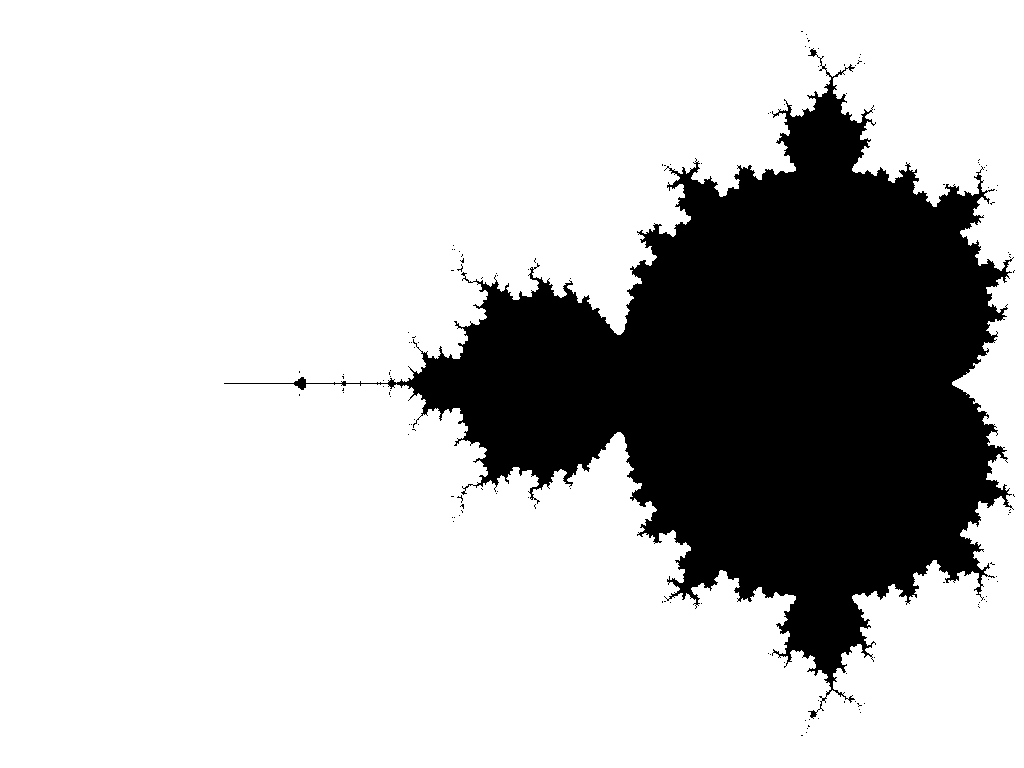
\includegraphics[width=0.7\textwidth]{figures/Mandelbrot_black.png}
  \caption{The Mandelbrot set over $c_r \in [-2.5, 1.0]$, $c_i \in [-1.25, 1.25]$}
  \label{fig:mandelbrot-set}
\end{figure}

$M$ has a few properties that matter directly for rendering it, all visible directly in
Figure~\ref{fig:mandelbrot-set}. First, it is bounded. If $|c| > 2$, the sequence in
Equation~\ref{eq:mandelbrot-iteration} is guaranteed to diverge, so $M$ lies entirely within the
disk $|c| \leq 2$. This follows because once $|z_n| > 2$ and $|z_n| \geq |c|$, each further step at
least multiplies the distance from the origin by a factor bigger than $1$, so $|z_n|$ grows without
bound. The same argument is what justifies stopping the iteration early for any pixel once $|z_n|$
crosses that threshold, instead of iterating forever. Second, $M$ is connected. Despite its visually
disconnected looking "islands," every point of the set can be joined to every other point by a
path that stays inside $M$, a result proved by Douady and Hubbard through the set's uniformization
by external rays. Third, $M$ is self similar in a loose sense. Its boundary contains infinitely many
small, distorted copies of the whole set, at every scale, known as satellite or "mini-Mandelbrot"
copies. This is precisely why zooming into the boundary keeps revealing new detail rather than
converging to a simple curve. It is also the reason deep zoom rendering, Section~\ref{sec:perturbation},
is an interesting problem at all, not just a matter of computing the same picture at a smaller
scale. Finally, although $M$ is a two dimensional region of the plane, its boundary is a fractal
curve of Hausdorff dimension exactly $2$. A curve that space filling is,
informally, why the escape time test near the boundary is numerically delicate and why the pixels
that take the longest to classify are concentrated exactly where the image has the most visual
detail.

\section{Escape Time Rendering Basics}
\label{sec:escape-time-basics}

Equation~\ref{eq:mandelbrot-iteration} cannot be iterated forever on a real computer, so a
renderer has to turn the exact yes or no membership test into two practical approximations.

The first is a bailout. Instead of waiting for $|z_n| \to \infty$, the iteration stops as soon as
$|z_n|$ crosses a fixed escape radius. A radius of $2$ is already enough to guarantee that the
point will diverge, by the same argument used in Section~\ref{sec:mandelbrot-definition}, so any
larger radius is a safe, if sometimes unnecessary, choice. Renderers that want smoother colouring
often bail out at a larger radius on purpose, at the cost of a handful of extra iterations per
escaping pixel. The second approximation is a maximum iteration count. A pixel that has not escaped
once this limit is reached is treated as being inside the set, even though a slightly higher limit
might eventually show it escaping. Raising the limit makes the picture more accurate, particularly
near the boundary and at deep zoom, but also makes every pixel that never escapes, typically the
majority of the image at high zoom, proportionally more expensive to render. The number of
iterations executed is therefore far from uniform across the image. Pixels far from $M$ escape
almost immediately, pixels deep inside it run the full iteration limit, and pixels near the
boundary can do either, unpredictably. This workload imbalance is the main reason naive per pixel
parallelization performs poorly, and it is the underlying problem that the optimizations in
Chapter~\ref{ch:algorithms} and the scheduler in Chapter~\ref{ch:scheduler} both work around.

Turning the raw iteration count into a picture also needs care. Mapping the integer iteration count
directly to a colour produces visible banding, sharp rings where the count changes by one, instead
of a smooth gradient. The standard fix is smooth, or "normalized," colouring, which uses the
escaped value of $z_n$ to compute a fractional iteration count
\begin{equation}
  \label{eq:smooth-coloring}
  \nu = n + 1 - \frac{\log \log |z_n|}{\log 2},
\end{equation}
so that neighbouring pixels that escaped after, say, $41.3$ and $41.7$ iterations get visibly
different, interpolated colours instead of being lumped into the same band. The range of
$\nu$ values present in a frame changes completely with zoom level and location. Mapping $\nu$ to a
colour palette well typically also needs a normalization step, for example histogram equalization.
This ensures the available palette entries are spent where the image actually has detail, rather
than on iteration counts that barely occur in that particular frame.

\begin{figure}[H]
  \centering
  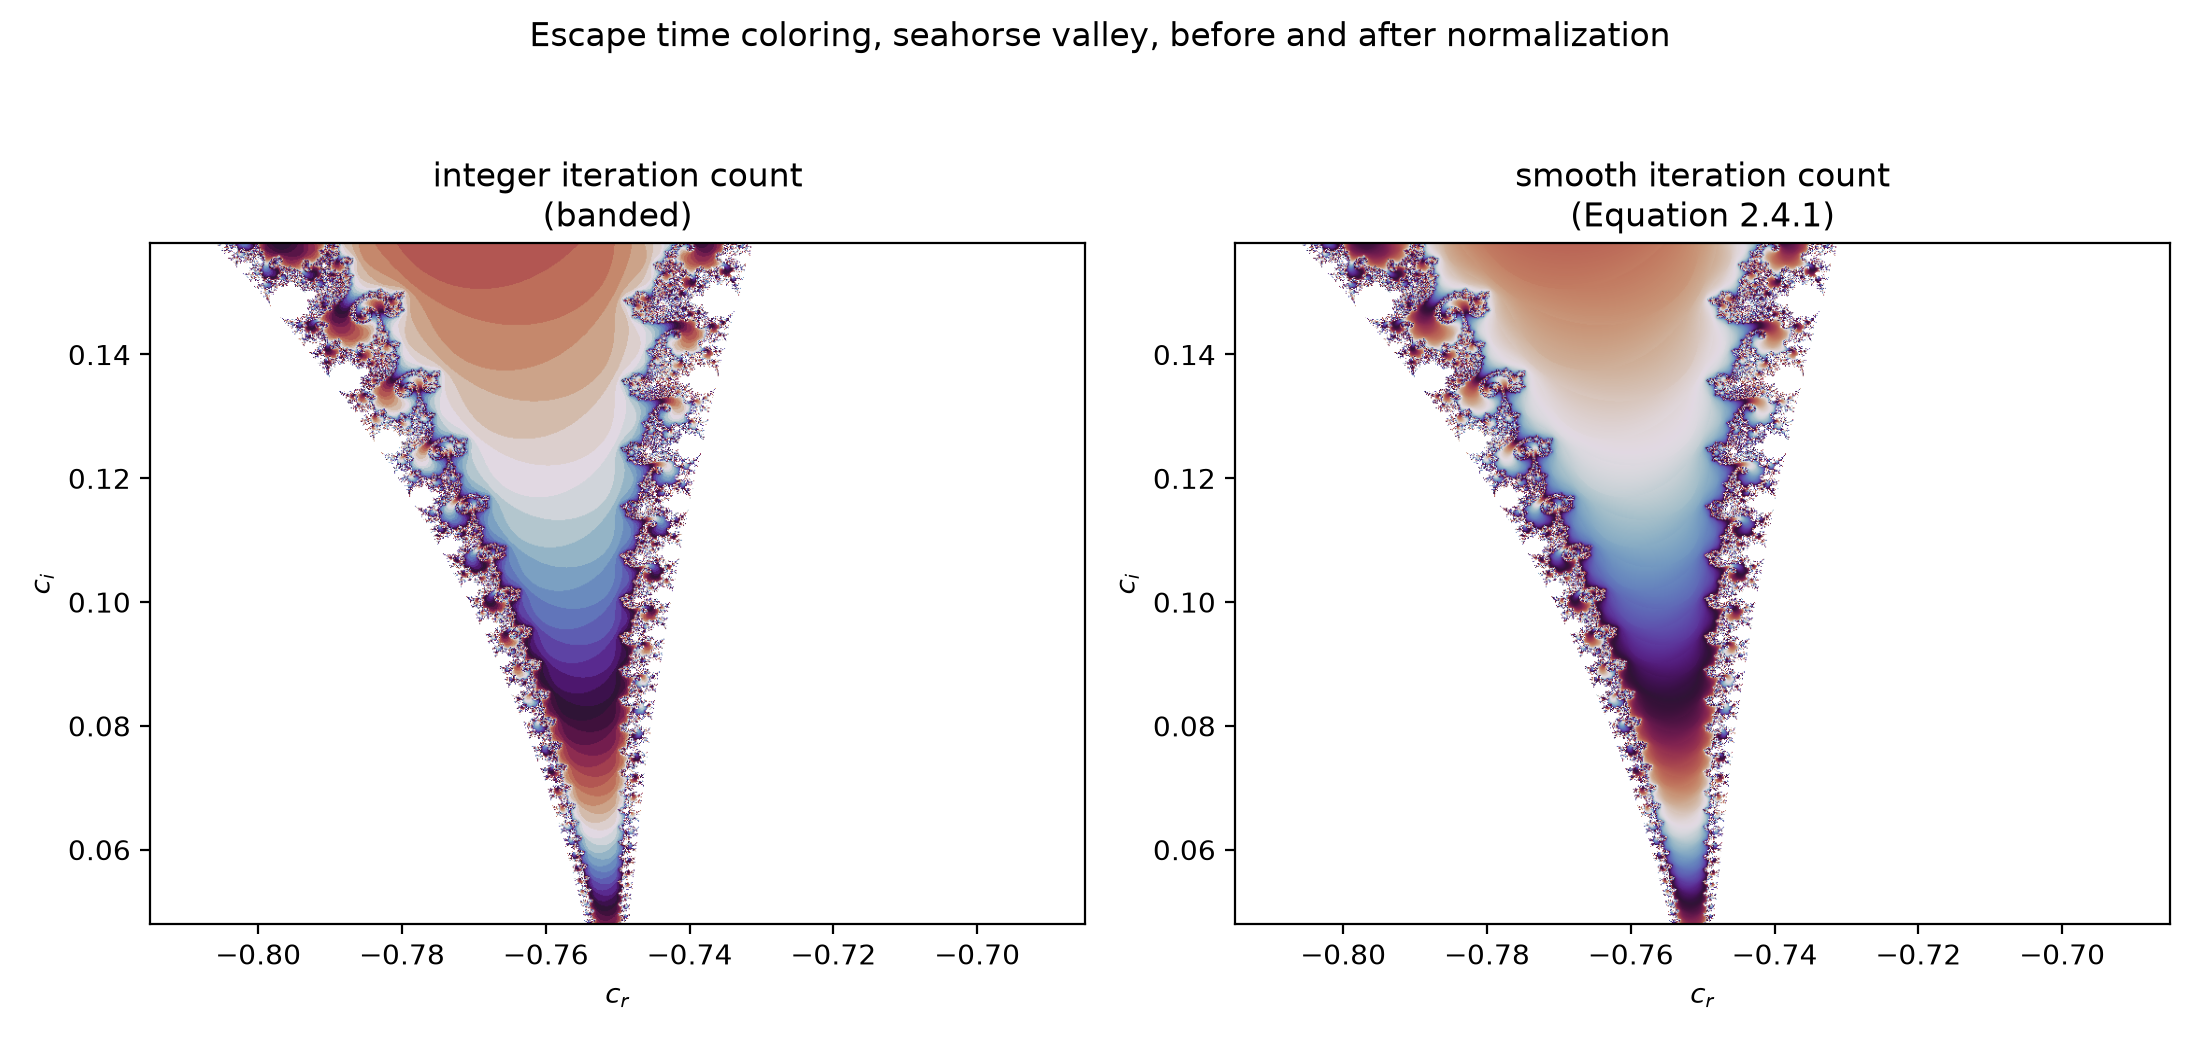
\includegraphics[width=\textwidth]{figures/escape-time-banding.png}
  \caption{The same boundary region coloured by raw integer iteration count and by the smooth count
  from Equation~\ref{eq:smooth-coloring}. The left
  image's rings are the palette repeating once per whole iteration. The right image cycles through
  the identical palette but interpolates within each ring.}
  \label{fig:escape-time-banding}
\end{figure}

\chapter{Rendering Algorithms}
\label{ch:algorithms}

\section{Baseline Scalar Escape Time}
\label{sec:baseline-scalar}

The renderer's baseline is a direct, unvectorized implementation of the iteration in
Equation~\ref{eq:mandelbrot-iteration}, one \kod{f64} complex number per pixel, one pixel at a
time. Two things separate it from a textbook loop, and both matter for what "baseline" means for
the rest of this chapter. First, before iterating at all, it runs the analytic early exit tests
from Section~\ref{sec:early-exit}, so the baseline already excludes the two largest interior
components of the set from the iteration loop. Every later optimization in this chapter is
measured against a baseline that already has this test, not against a naive loop with no
shortcuts. Second, the update step $z_{n+1} = z_n^2 + c$ is written as a single fused multiply-add
instruction rather than a separate multiply and add, so the hardware does one rounding step instead
of two.

The escape test itself uses the radius established in Section~\ref{sec:escape-time-basics},
$|z_n|^2 > 4$, checked as a squared comparison to avoid a square root every iteration. On top of
the bailout, the renderer runs Brent style cycle detection \cite{brent1980}. Every few iterations
it stores the current $z_n$, and on later iterations compares against that saved value. If the
orbit returns to within $10^{-20}$ of it, the point is periodic and is immediately classified as
being in the set, without waiting for \kod{max\_iter}. The comparison interval starts at $8$
iterations and doubles after each check, capped at $512$. This way the check runs often while it is
likely to pay off early and rarely later, once it is unlikely to trigger and would otherwise add
per iteration overhead for no benefit. This catches the cycles the cardioid and bulb tests miss.
Those tests are closed form for the two largest components of the set. The boundary, though,
contains infinitely many smaller periodic components, the visible smaller bulbs and the tiny
satellite copies from Section~\ref{sec:mandelbrot-definition}, that Brent's method can still catch
generically, without knowing their shape in advance.

Work is split across CPU cores in data parallel row chunks, and the pixel loop itself does no per
pixel division or trigonometry. The mapping from pixel coordinates to a complex number is reduced,
once per frame, to four constants, the real and imaginary start and step, so each pixel's
coordinate is one multiply-add away from the previous one. On the reference machine used throughout
this thesis, Chapter~\ref{ch:methodology}, this baseline sustains roughly $195$ to $239$ million
pixels per second across resolutions from $800\times600$ to $3840\times2160$ for Mandelbrot at
$1000$ iterations. Throughput is essentially flat with resolution, which is expected for a workload
where each pixel's cost does not depend on the size of the image around it.

\section{SIMD Vectorization}
\label{sec:simd}

The scalar loop in Section~\ref{sec:baseline-scalar} computes one pixel's iteration at a time even
though modern CPUs can apply the same arithmetic operation to several values in a single
instruction. The renderer's SIMD kernels replace the scalar $z_{n+1}=z_n^2+c$ update with the same
update applied to several pixels at once, packed into one vector register, \kod{f64x4} with four
\kod{f64} lanes and \kod{f32x8} with eight \kod{f32} lanes. Which one runs depends on zoom depth,
via the same $10^6$ threshold used throughout this thesis to choose between \kod{f32} and
\kod{f64}. Below it, the renderer uses the wider, cheaper \kod{f32x8} kernel. Above it,
\kod{f32}'s roughly seven decimal digits of precision are no longer enough to tell neighbouring
pixels apart, so it falls back to \kod{f64x4}.

Vectorizing the escape time loop raises a problem the scalar loop does not have. Different lanes
escape at different iteration counts, but a SIMD instruction applies the same operation to every
lane at once, so no single lane can stop early on its own. The kernels solve this with an active
lane mask, a per lane bit pattern of all ones or all zeros, combined with the update via a bitwise
AND. Once a lane's $|z_n|^2$ crosses the escape radius, its escape iteration and value of $z_n$ are
recorded and the mask clears that lane, so further updates to it become no-ops while the remaining
lanes keep going. The loop only stops once every lane has escaped or \kod{max\_iter} is reached.

A third kernel, used only for Mandelbrot, pushes further by running two independent \kod{f32x8}
chains side by side, sixteen pixels per step rather than eight. The two chains are otherwise
identical. The point is instruction level parallelism, not extra vector width. Modern CPUs can have
several fused multiply-add instructions in flight at once if a second, independent chain of work is
available to fill the pipeline while the first chain's result is still being computed. Measured on
$1920\times1080$ Mandelbrot at $1000$ iterations, the two chain kernel renders a frame in
$4.25\,\mathrm{ms}$, against $4.62\,\mathrm{ms}$ for the single \kod{f32x8} kernel,
$6.04\,\mathrm{ms}$ for \kod{f64x4}, and $8.17\,\mathrm{ms}$ for the scalar baseline, a $1.92\times$
speedup over scalar, of which only about $8\%$ comes from the second chain itself. That the added
gain from instruction level parallelism is small is not a surprise once Section~\ref{sec:early-exit}
is taken into account. The cardioid and bulb tests already remove a large share of the interior
pixels before the hot loop runs at all, leaving less latency left for a second chain to hide. One
criterion run during benchmarking also showed two supposedly identical, repeated measurements of
the same kernel disagreeing by more than half. Chapter~\ref{ch:methodology} returns to this as a
reminder that a single benchmark run is noise until it has been repeated.

\section{Geometric Early Exit Tests}
\label{sec:early-exit}

Two regions of the Mandelbrot set are large enough, and simple enough in shape, that membership can
be tested directly from $c$ without iterating at all, a standard acceleration described in
\cite{peitgensaupe1988}. The main cardioid, the largest component, is
the image of the unit circle under $c = \tfrac{1}{2}e^{i\theta} - \tfrac{1}{4}e^{2i\theta}$.
Equivalently, writing $q = (c_r - 0.25)^2 + c_i^2$, a point lies in the cardioid exactly when
\begin{equation}
  \label{eq:cardioid-test}
  q \, (q + c_r - 0.25) < 0.25 \, c_i^2 .
\end{equation}
The period 2 bulb, the large circular component attached to the cardioid's left side, is exactly a
disk, $(c_r + 1)^2 + c_i^2 < 0.0625$, of radius $0.25$ centred at $c = -1$. Both tests are exact
algebraic identities, not approximations, so any point they classify as interior really is
interior, and can be assigned \kod{max\_iter} directly, with no iteration at all.

The renderer also tests the two period 3 bulbs, the next largest interior components, attached to
the cardioid above and below the period 2 bulb. They do not have as clean a closed form as the
cardioid, but each is still well approximated by a disk, centred near $c \approx (-0.122561,
\pm0.744862)$ with radius $\approx 0.073715$. Testing squared distance against a squared radius
again avoids a square root. Past period $3$, the boundary keeps producing smaller bulbs and
satellite copies without end, Section~\ref{sec:mandelbrot-definition}, and it stops being worth
hand deriving a closed form test for each one. Smaller periodic components are instead caught
generically by the cycle detection already built into the baseline, Section~\ref{sec:baseline-scalar}.

These three tests run first, before the iteration loop, on every pixel in every kernel in this
chapter, scalar and SIMD alike. The cardioid and period 2 tests vectorize directly, since they are
just arithmetic on the SIMD lanes. The period 3 test, whose disk centres do not vectorize as
cleanly, is instead evaluated per lane in scalar precision, only for the pixels the first two tests
did not already resolve. The main cardioid and the period 2 bulb are the two largest regions of the
set by area. This test alone therefore accounts for a large share of the pixels that would
otherwise run to \kod{max\_iter} doing no useful work, exactly the heavy pixels identified as the
main source of the workload imbalance in Section~\ref{sec:escape-time-basics}.

\begin{figure}[H]
  \centering
  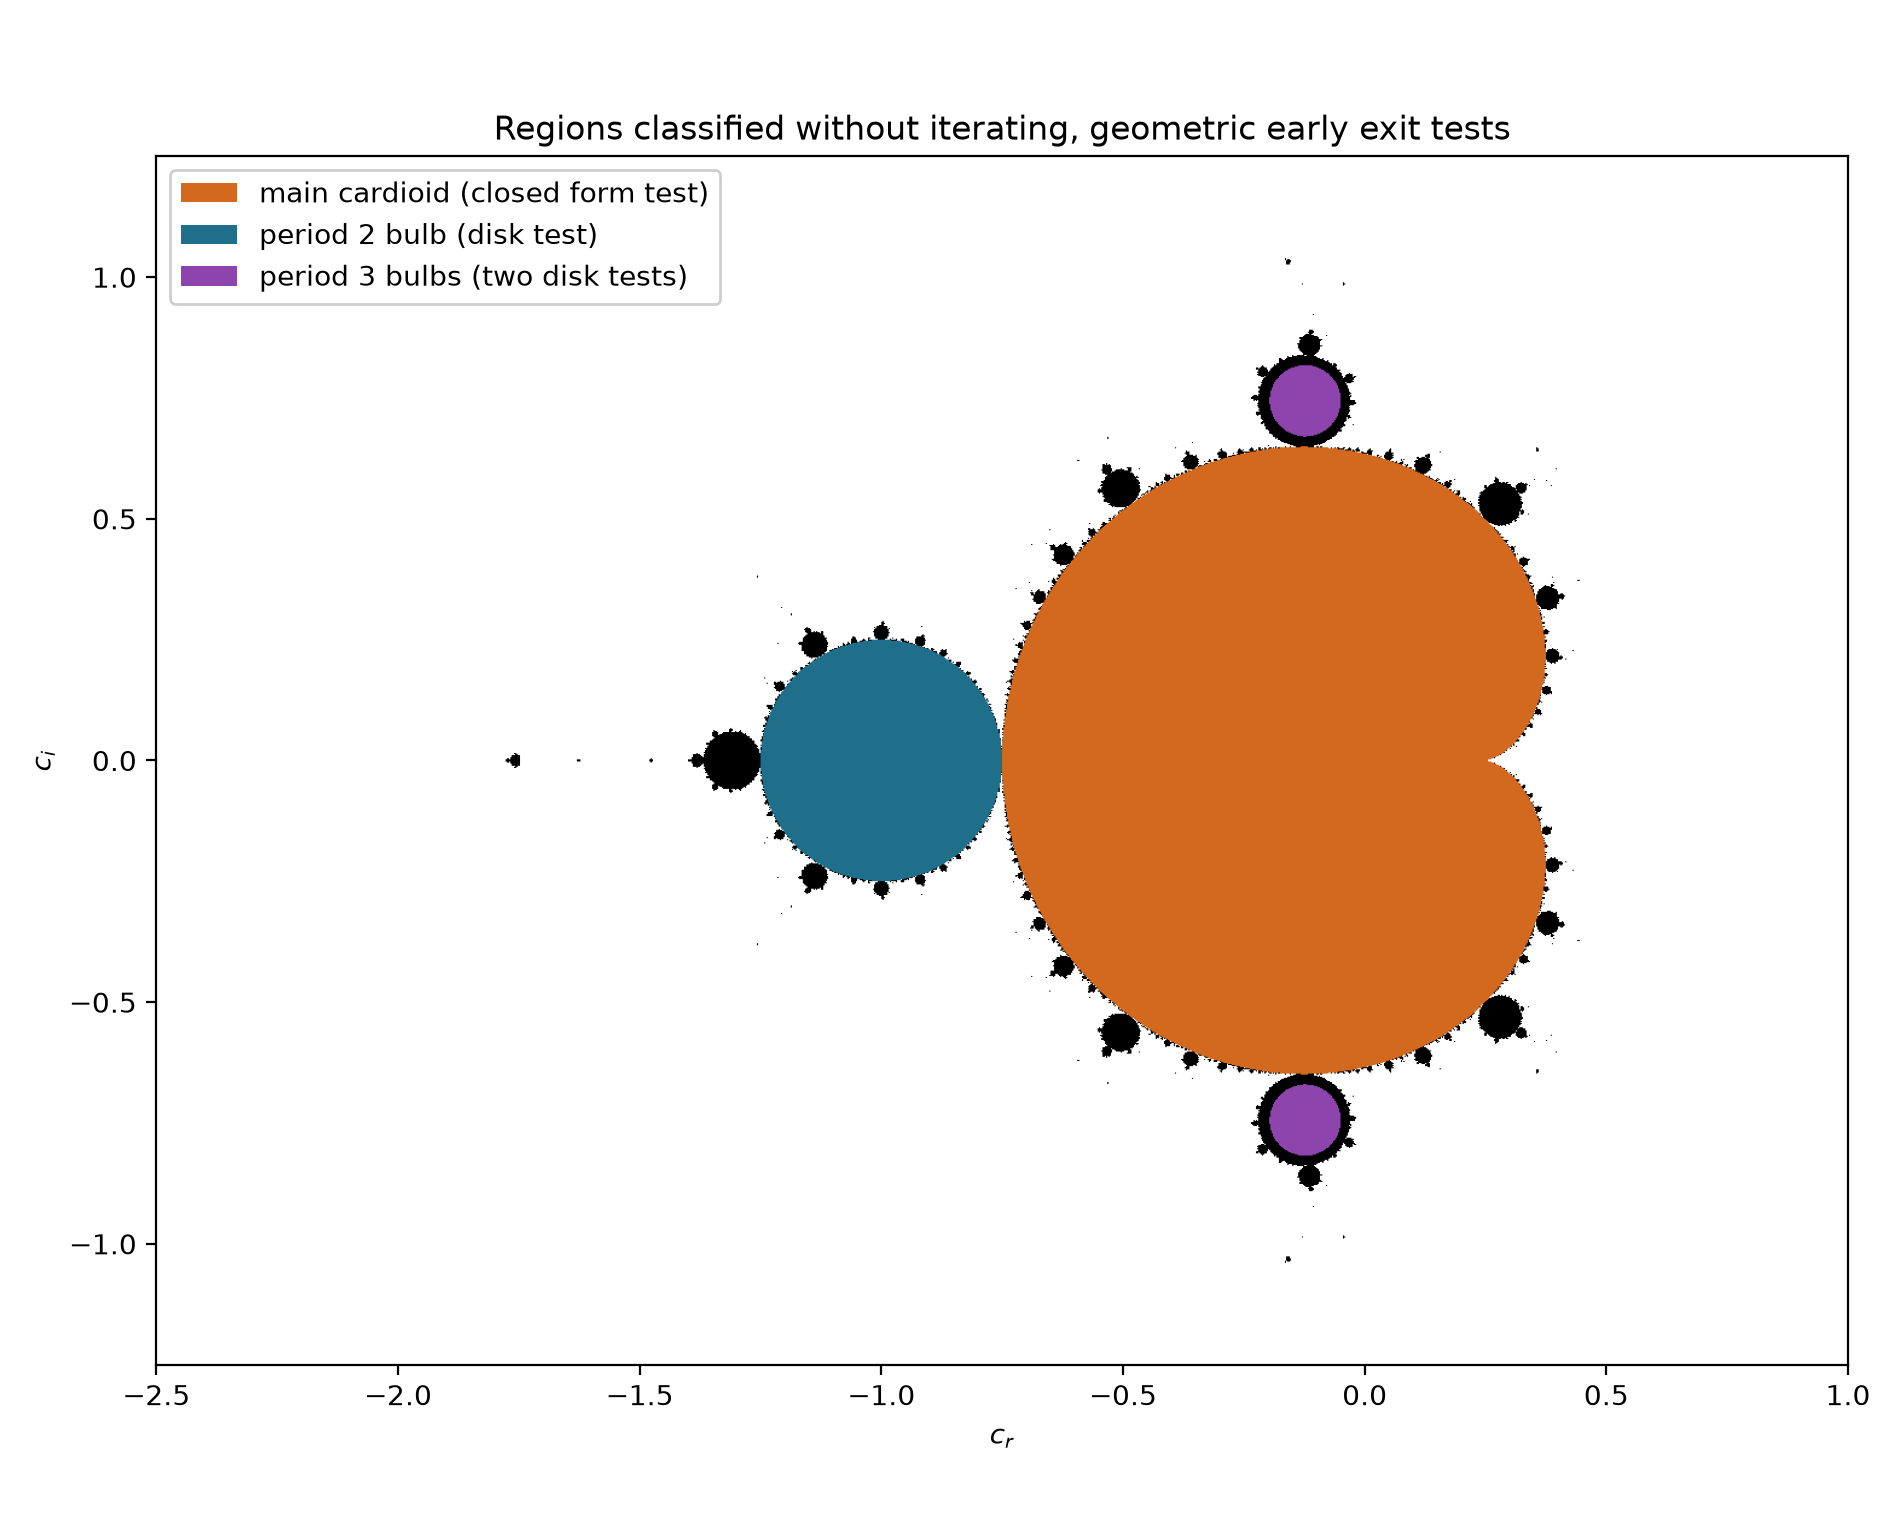
\includegraphics[width=0.85\textwidth]{figures/alg-early-exit-regions.png}
  \caption{The three closed form regions over a full frame Mandelbrot render, main cardioid, period
  2 bulb, and the two period 3 bulbs. Every pixel inside a shaded region is assigned \kod{max\_iter}
  directly, with no iteration at all. Everywhere else, including the smaller satellite bulbs visible
  along the boundary, still runs the full loop.}
  \label{fig:early-exit-regions}
\end{figure}

\section{Mariani-Silver Boundary Subdivision}
\label{sec:mariani-silver}

The tests in Section~\ref{sec:early-exit} classify individual pixels as interior in closed form.
Mariani-Silver subdivision \cite{peitgensaupe1988} instead exploits the fact that large regions of
the \emph{exterior} of the set, far from the boundary, also share the same escape iteration count
as their neighbours. The algorithm then tries to detect and fill such regions without computing
every pixel inside them.

Given a rectangle of the image, the algorithm renders only its border, the top and bottom rows and
the left and right columns. If every border pixel has the same value, the rectangle is assumed
uniform and its whole interior is filled with that value without ever touching the pixels inside
it. If the border is not uniform, the rectangle is too small to make that assumption safely. It is
split in two along its longer axis instead, keeping the two halves closer to square rather than
producing long slivers, and the same test is applied recursively to each half. This continues down
to a minimum size of $2\times2$ pixels, below which subdivision no longer pays for itself and the
remaining pixels are simply computed directly. Adjacent rectangles share a border, so the frame buffer is
seeded in advance with a sentinel value, and a border pixel already computed by a neighbouring rectangle
is never recomputed.

\begin{figure}[H]
  \centering
  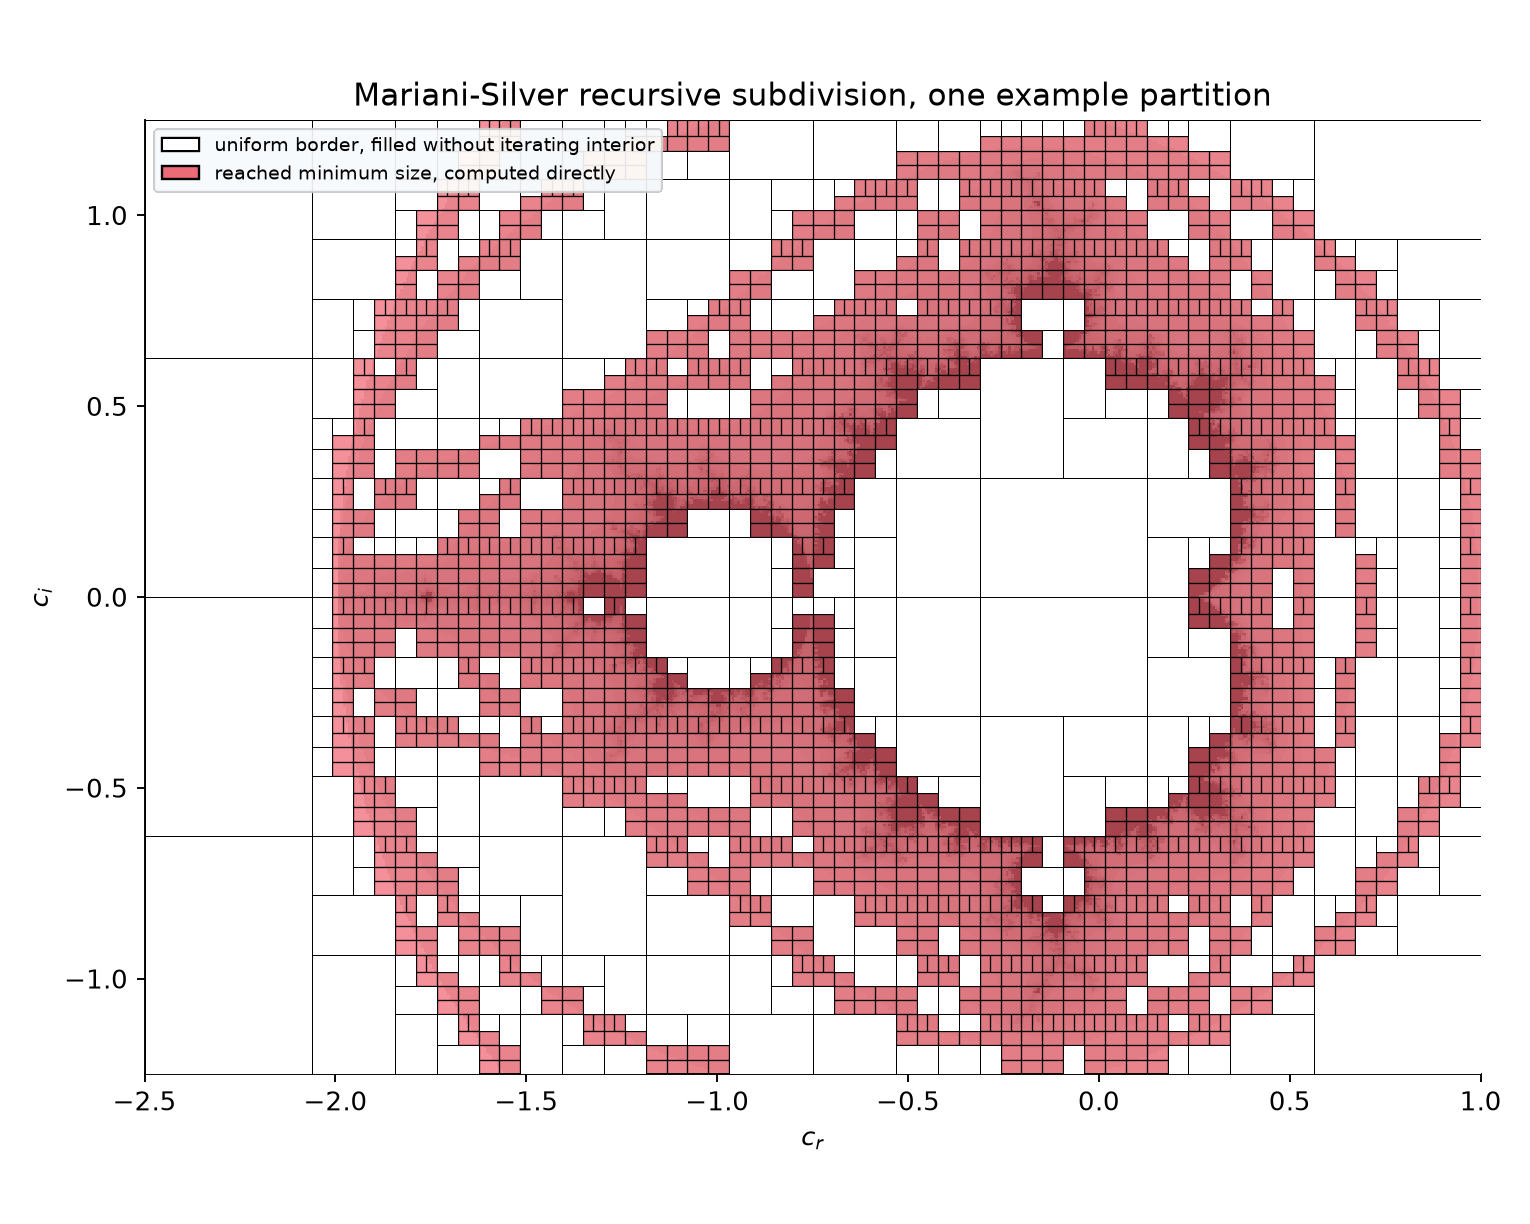
\includegraphics[width=0.85\textwidth]{figures/alg-mariani-silver-example.png}
  \caption{One example partition over a full frame Mandelbrot render, minimum size raised to
  $6\times6$ pixels here for visibility, the renderer itself stops at $2\times2$. White rectangles
  had a uniform border and were filled without touching their interior. Red rectangles reached the
  minimum size and were computed directly.}
  \label{fig:mariani-silver-example}
\end{figure}

The uniform border assumption is not strictly guaranteed. In principle a thin filament of
differently valued pixels could thread through a rectangle's interior without ever touching its
border, in which case the fill step would paint over it. In practice this is rare enough, and the
visual cost small enough, that the algorithm accepts it as a known, bounded risk approximation
rather than guarding against it explicitly.

A second variant folds in the distance estimate from Section~\ref{sec:dem}. Instead of only
checking whether the border is uniform, it also checks whether every corner of the rectangle is
farther from the set's boundary than the rectangle's own diagonal, scaled by a tunable safety
margin $k$. If so, the whole rectangle is known to be far enough from any boundary detail that a
bilinear interpolation between the four corner values is visually indistinguishable from computing
every pixel. The rectangle is filled that way instead, with a sanity check that the corners'
smooth iteration counts do not differ by more than $2.0$. This check matters because a bilinear
fill across a region where the underlying function changes quickly would visibly misrender it.

\section{Distance Estimation Method}
\label{sec:dem}

The distance estimation method \cite{peitgensaupe1988} answers a different question than the
escape time test, not how many iterations until $c$ escapes, but how far $c$ is from the boundary
of the set. This quantity's rigorous justification comes from the potential theory of the set's
exterior \cite{milnor2006}. The estimate follows from tracking, alongside the ordinary orbit
$z_{n+1} = z_n^2 + c$, its derivative with respect to $c$.
\begin{equation}
  \label{eq:dem-derivative}
  z_0 = 0, \quad \frac{dz_0}{dc} = 0, \qquad
  z_{n+1} = z_n^2 + c, \quad \frac{dz_{n+1}}{dc} = 2 z_n \frac{dz_n}{dc} + 1,
\end{equation}
obtained by differentiating the iteration itself term by term. If the orbit escapes at iteration
$n$, the distance from $c$ to the nearest point of the boundary is approximately
\begin{equation}
  \label{eq:dem-distance}
  d \approx \frac{|z_n| \, \ln |z_n|}{|dz_n/dc|} .
\end{equation}

This is a standard result for the exterior distance estimate of an escape time fractal, not
specific to this renderer. What is specific to this renderer is how it gets used. Rather than
driving a dedicated anti-aliasing or outline rendering mode, $d$ is used exactly once, as the cull
test inside the DEM augmented Mariani-Silver variant from Section~\ref{sec:mariani-silver}. A
rectangle whose four corners are all farther from the boundary than their own diagonal is
guaranteed not to contain any fine boundary detail, and can safely be filled by interpolation
instead of iterated pixel by pixel. Because $dz_n/dc$ is accumulated with one extra complex
multiply-add per iteration on top of the ordinary orbit, the distance estimate is nearly free to
compute alongside an escape time run that was going to happen anyway. The actual saving comes from
how much pixel by pixel work the culling test lets Mariani-Silver skip, not from the estimate
itself being cheap in isolation.

\section{Perturbation Theory}
\label{sec:perturbation}

Every kernel described so far iterates $c$ directly in \kod{f64} or \kod{f32}, which stops working
once the zoom is deep enough that neighbouring pixels' $c$ values differ by less than a double
precision float can resolve. That limit is reached long before the deep zoom regime that
Section~\ref{sec:mandelbrot-definition}'s self similar boundary makes interesting. Perturbation
theory \cite{martin2013superfractalthing} sidesteps this by iterating a \emph{difference} instead
of an absolute value. A single high precision reference orbit $Z_n$ is computed once, for one
reference point near the centre of the view. Every other pixel $c = c_{\mathrm{ref}} + \delta c$
is then rendered by iterating the much smaller quantity $\delta_n = z_n - Z_n$ directly.
\begin{equation}
  \label{eq:perturbation}
  \delta_{n+1} = 2 Z_n \delta_n + \delta_n^2 + \delta c ,
\end{equation}
obtained by subtracting the reference orbit's own recurrence from the pixel's. Because $\delta_n$
stays small for most pixels near the reference point, it can be iterated in ordinary \kod{f64}
even where the corresponding $z_n$ itself would have needed far more precision to represent. This
means the expensive high precision work Section~\ref{sec:precision} is paid for once per frame
instead of once per pixel.

\begin{figure}[H]
  \centering
  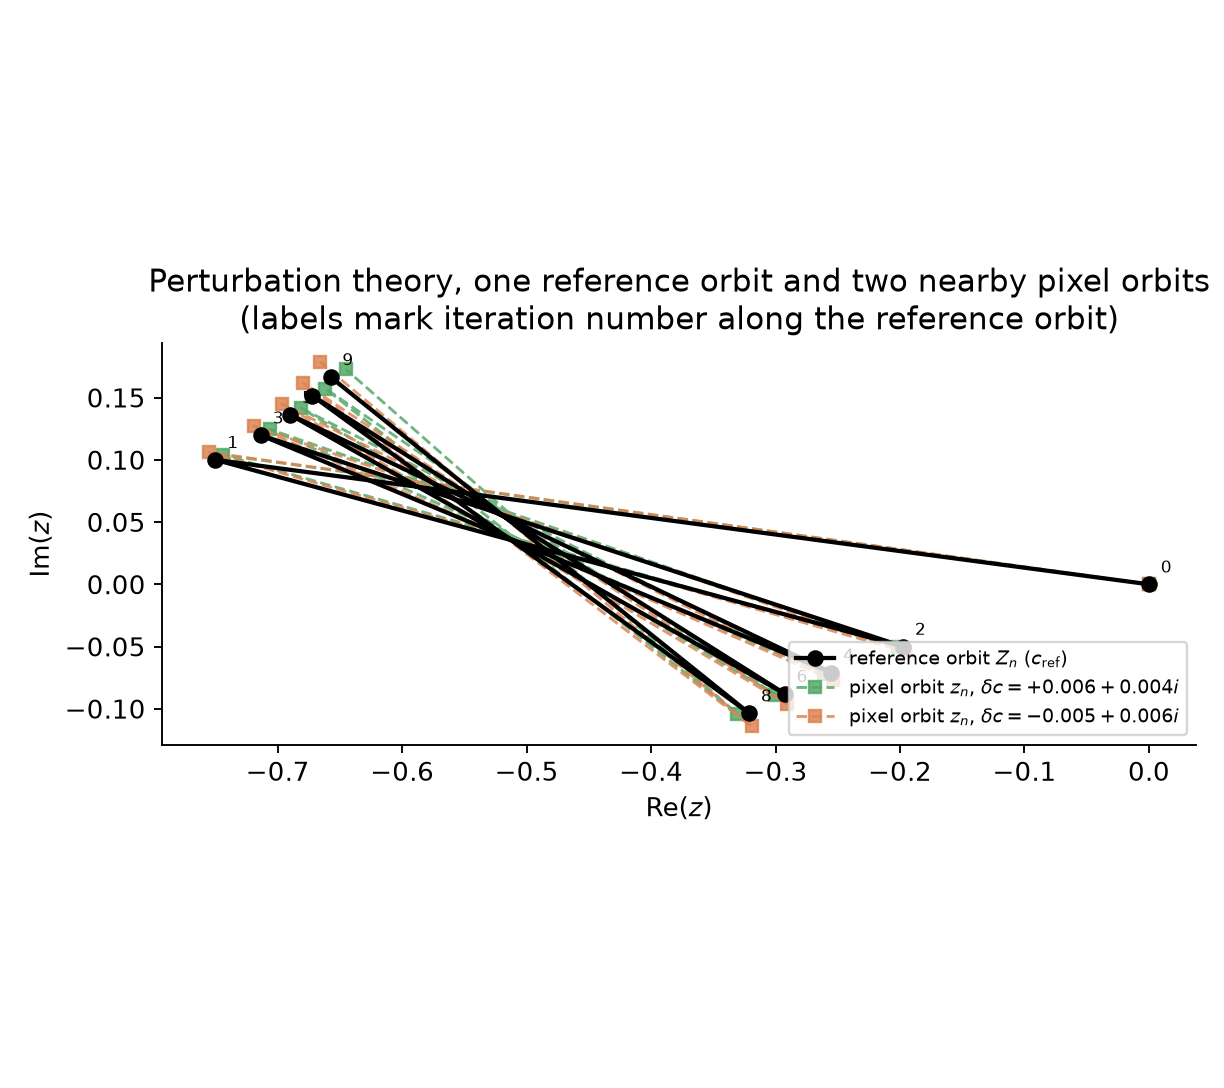
\includegraphics[width=0.7\textwidth]{figures/perturbation-schematic.png}
  \caption{A real reference orbit at $c_{\mathrm{ref}}=-0.75+0.1i$, the seahorse valley point
  Section~\ref{sec:bench-viewports} also uses, alongside two pixel orbits a small $\delta c$ away.
  All three orbits stay close together for the iterations shown, which is exactly what lets
  $\delta_n$ be represented in ordinary \kod{f64} while $Z_n$ itself carries the extended precision.}
  \label{fig:perturbation-schematic}
\end{figure}

This breaks down for pixels whose orbit drifts too far from the reference. Once $|\delta_n|$ grows
to a non negligible fraction of $|Z_n|$, the approximation the method relies on stops holding, an
event usually called a \emph{glitch}. The renderer detects this by comparing $|\delta_n|^2$ against
a small fixed fraction of $|Z_n|^2$ and flags the pixel once it is crossed. The plain variant
simply falls back to the exact scalar kernel from Section~\ref{sec:baseline-scalar} for any flagged
pixel, which is always correct but pays the full per pixel cost again for exactly the pixels
perturbation was meant to avoid computing directly. \emph{Rebasing} \cite{heilandallen2021deepzoom}
avoids most of that fallback without a second reference orbit. Whenever a pixel's orbit happens to
pass close to the origin again, once $|z_n|^2$ drops back below $|\delta_n|^2$, or the stored
reference orbit runs out, the current $z_n$ is simply adopted as a new, local delta of $0$, and
iteration continues against the same reference orbit from that point on, reusing one precomputed
orbit as though a fresh reference had been recomputed there for free. \emph{Multi-reference}
rendering goes further still. It renders the whole frame against one reference, marks every
glitched pixel, and then computes a new reference centered on the first pixel still glitched, since
glitches cluster spatially as nearby pixels tend to drift away from a given reference together,
repeating up to $8$ reference orbits before giving up and falling back to the exact kernel for
whatever is still unresolved.

Measured directly, perturbation rendering is not a throughput win. Across the zoom range tested, it
renders slower than the direct kernel it replaces, because that range never reaches the depth where
\kod{f64} actually breaks down, so the perturbation machinery is pure overhead on top of arithmetic
the direct kernel could already do unaided.

\section{Series Approximation}
\label{sec:series-approximation}

Perturbation iteration from Section~\ref{sec:perturbation} still runs one $\delta_n$ update per
pixel per iteration. Series approximation \cite{martin2013superfractalthing,
heilandallen2021deepzoom} tries to skip the first several hundred iterations of that work
entirely, for pixels close enough to the reference orbit that their early behaviour is predictable
in closed form.

Substituting a power series guess $\delta_n \approx A_n \delta c + B_n \delta c^2 +
C_n \delta c^3 + D_n \delta c^4$ into the perturbation recurrence Equation~\ref{eq:perturbation}
and matching powers of $\delta c$ gives a recurrence for the coefficients themselves, computed once
alongside the reference orbit.
\begin{align}
  \label{eq:sa-coefficients}
  A_{n+1} &= 2 Z_n A_n + 1, &
  B_{n+1} &= 2 Z_n B_n + A_n^2, \\
  C_{n+1} &= 2 Z_n C_n + 2 A_n B_n, &
  D_{n+1} &= 2 Z_n D_n + \left(2 A_n C_n + B_n^2\right).
\end{align}
As long as the third and fourth order terms stay negligible relative to the leading term for the
worst case $\delta c$ in the frame, the viewport corner farthest from the reference point, the
series is a valid stand in for direct iteration. The renderer tracks the last iteration at which
that holds, evaluates the series directly at that iteration for every pixel, and then continues
ordinary perturbation iteration from there instead of from iteration zero.

On the benchmark scene used for perturbation above, the skippable prefix turns out to be short. It
runs to a few tens of iterations out of a thousand, a one to three percent head start rather than
the large upfront skip series approximation is capable of at greater depth.

\section{Numerical Precision for Deep Zoom}
\label{sec:precision}

Perturbation theory, Section~\ref{sec:perturbation}, moves the precision problem rather than
eliminating it. Pixel deltas can stay in \kod{f64}, but the single reference orbit they are
computed against still has to track an absolute position in the complex plane, and at extreme zoom
that position needs more than \kod{f64}'s roughly $53$ bits of mantissa to distinguish from its
neighbours. Rather than pull in an arbitrary precision arithmetic library, the renderer represents
an extended precision real number the way Dekker's classic double-double technique does
\cite{dekker1971}, as an unevaluated pair of ordinary \kod{f64} values, $(hi, lo)$, with the
invariant that $|lo|$ is at most half a unit in the last place of $hi$. The true value is the exact
sum $hi + lo$, which is never actually computed as a single float. This "double-double"
representation gives roughly $106$ bits of mantissa, twice \kod{f64}'s, while every individual
operation on it still runs as ordinary hardware floating point arithmetic.

The two building blocks are Knuth's \kod{TwoSum} \cite{knuth1997seminumerical}, a short branch
free sequence that computes $a+b$ together with its exact rounding error in a second float, and a
\kod{TwoProduct} \cite{ogitarumpoishi2005} that gets the same exact error decomposition for a
multiplication directly from a fused multiply-add. It computes $p = a \times b$ and then the error
term as $a \times b - p$ in a single fused multiply-add instruction, with no double width
intermediate needed. Addition on the pair type sums the high parts with \kod{TwoSum}, folds both
low parts into the resulting error term, and renormalizes with a second \kod{TwoSum}.
Multiplication computes the exact high part product with \kod{TwoProduct}, adds the cross terms
$hi_a \cdot lo_b$ and $lo_a \cdot hi_b$ as ordinary \kod{f64} products, already small enough not to
need their own error term, and renormalizes the same way.

This extended precision is used in exactly one place, computing the reference orbit itself, once
the requested zoom passes a fixed threshold, $10^{12}$, beyond which plain \kod{f64} is no longer
trustworthy for that orbit. Every per pixel $\delta_n$ update still runs in ordinary \kod{f64}
against that orbit, truncated back down from the pair representation once it is stored, since the
deltas themselves never needed the extra precision, only the shared reference did. Because the
reference orbit is computed once per frame rather than once per pixel, the roughly twofold
arithmetic cost of double-double operations over plain \kod{f64} stays negligible against total
frame time even when it is active.

\section{Traversal and Locality}
\label{sec:traversal-locality}

Every algorithm so far decides \emph{what} to compute for a pixel. This section is about the order
\emph{in which} pixels are visited, and about avoiding recomputation altogether when the previous
frame already contains most of the answer.

The renderer divides the frame into square tiles of $64 \times 64$ pixels and distributes bands of
tiles across CPU worker threads. This fixed tile size is also the unit of work the hybrid scheduler
in Chapter~\ref{ch:scheduler} dispatches to the CPU and the GPU. Within a tile, pixels can be
visited in plain row major order, or along a Hilbert curve \cite{hilbert1891}, a recursively
defined path that always steps to a geometrically adjacent pixel and, unlike row major order,
never jumps back across the full width of the tile at the end of a row. The Hilbert visiting order
for a tile is generated once by interleaving bits and rotating quadrants, and reused unchanged for
every tile in the frame, so the per pixel cost is only a table lookup, not a recomputation of the
curve.

\begin{figure}[H]
  \centering
  
\includegraphics[width=\textwidth]{figures/traversal-hilbert-vs-rowmajor.png}
  \caption{Pixel visiting order within one tile, row major against Hilbert. Row major jumps back
  across the full tile width at the end of every row. The Hilbert curve never takes a step that
  is not to a geometrically adjacent cell.}
  \label{fig:traversal-hilbert}
\end{figure}

The motivation for trying a Hilbert order at all is cache locality. Consecutive pixels along the
curve are also spatially close in the image, and if a full frame buffer does not fit in cache, that
should mean fewer evictions than a row major sweep that revisits a row's neighbourhood only after
scanning every other row in between. On this thesis's benchmark hardware, that expected win does
not appear. Hilbert traversal renders measurably slower than plain row major order at every
resolution tested, and its last level cache miss rate is higher, not lower. The most likely
explanation, examined in Chapter~\ref{ch:results}, is that the frame buffer at the tested
resolutions already fits comfortably in the CPU's last level cache with hardware prefetching doing
its job on the row major access pattern, so the Hilbert curve's per pixel bit interleaving becomes
pure added cost with no locality problem left for it to solve. A different traversal order, Morton
or Z-order indexing \cite{morton1966}, is used elsewhere in this renderer, but on the GPU rather
than the CPU tiling path described here. Section~\ref{sec:gpu-traversal} covers how it keeps
threads within a GPU warp accessing nearby memory.

Panning the view does not need to touch the traversal order at all, only the amount of work done.
When the view shifts along a single axis, most of the previous frame's pixels reappear at a shifted
position rather than needing to be recomputed. The renderer copies the reusable region of the old
buffer into its new position with a single bulk memory copy and only computes the newly exposed
strip along the edge the view moved toward. This turns a full frame recompute into a copy plus a
recompute proportional to the pan distance rather than the frame area, but only for panning aligned
to one axis. A simultaneous horizontal and vertical shift would need the reused and newly exposed
regions expressed as an overlapping copy that a single bulk copy cannot represent, so diagonal
panning falls back to computing the frame directly rather than attempting a partial reuse that
would not save the intended work anyway.

\chapter{GPU Implementation}
\label{ch:gpu}

\section{WebGPU Kernels}
\label{sec:webgpu}

WebGPU is the portable one of the renderer's two GPU backends. The same compiled shader runs on any GPU
with a Vulkan, Metal, or DirectX driver, at the cost of one hard restriction. WGSL, the shader
language WebGPU compiles, has no \kod{f64} type at all, so every kernel in this backend is
\kod{f32} only. Unlike the CPU and CUDA backends, this backend has no deep zoom fallback of its
own. It stays inside the same $10^6$ zoom threshold used throughout this thesis for the \kod{f32}
fast path, and anything beyond that threshold renders on a different backend entirely.

Within that limit, the WebGPU kernel mirrors the CPU's own \kod{f32} kernels closely. It runs the
same cardioid, period 2, and period 3 tests from Section~\ref{sec:early-exit}, inlined directly into the
shader, and it skips periodicity detection the same way the CPU's SIMD kernels do, on the same
reasoning that Brent's cycle check is not worth the extra branching at \kod{f32} granularity.
The Mandelbrot kernel shares its shader file with the renderer's other fractal types, selected at
runtime by an integer field in a small uniform buffer of view and rendering parameters uploaded
once per frame. Two entry
points share this kernel code. One dispatches one thread per pixel over the whole frame in
row major order, in workgroups of $16 \times 16$. The other instead reads an uploaded array of tile
descriptors and uses each workgroup's position in the dispatch to select one, bounds checking each
thread's local position against that tile's own width and height before writing to its true
position in the frame buffer. This second entry point is what the heterogeneous scheduler's GPU
worker dispatches through (Chapter~\ref{ch:scheduler}), since it needs to render an
arbitrary, scheduler chosen batch of tiles in one call rather than the whole frame.

A separate shader handles perturbation rendering. It uploads the reference orbit
(Section~\ref{sec:perturbation}) as two \kod{f32} arrays for the real and imaginary parts, together with
its center, and iterates the same delta recurrence, Equation~\ref{eq:perturbation}, that the CPU
kernels do, falling back to a direct \kod{f32} Mandelbrot evaluation on a glitch or once the
uploaded orbit runs out. It does not rebase and does not retry with a second reference. Unlike the
CPU path's three variants, WebGPU perturbation uses a single reference only. Rebasing and
multiple references would add control flow that needs to run identically across every thread in a
workgroup to stay cheap on a GPU, and this was not judged worth it for a backend whose reach is already
capped by \kod{f32}.

Getting the result back to the host costs more than computing it. The kernel writes into a
storage buffer on the GPU side. A copy from device to device then moves it into a second buffer flagged for
host mapping, which is mapped asynchronously and waited on before its contents are copied into a
freshly allocated host buffer. At $1920\times1080$, zoom $1$, \kod{max\_iter}~$=1000$, the kernel
itself runs in $0.29\,\mathrm{ms}$, but the full frame takes $2.26\,\mathrm{ms}$. Readback is
roughly $90\%$ of it.

\section{CUDA Backend}
\label{sec:cuda}

The CUDA backend targets the discrete NVIDIA GPU directly instead of going through a portability
layer. The kernel is compiled ahead of time with \kod{nvcc}, targeting the \kod{sm\_86}
architecture that matches the Ampere generation RTX 3050 this thesis benchmarks on, and the
resulting PTX is embedded into the compiled binary, so nothing needs compiling at runtime. Two of the compiler flags are
worth calling out on their own. One keeps denormalized floats alive, \kod{--ftz=false}, since the
smooth coloring formula from Section~\ref{sec:escape-time-basics} needs them for accuracy near the
escape threshold. The other turns fused multiply add contraction off entirely, \kod{--fmad=false}.
That second choice is the mirror image of Section~\ref{sec:baseline-scalar}'s
CPU kernel, which turns FMA \emph{on} for speed and accepts a difference of one rounding step from a
separate multiply and add. Here it is turned off so that CUDA's arithmetic rounds exactly the way
the CPU's does, trading a small amount of GPU throughput for images that are bit identical across
backends, which matters when the two are compared directly (Chapter~\ref{ch:results}).

Unlike the WebGPU backend, this backend keeps its default kernels in \kod{f64}, giving it full parity with the
CPU baseline. It runs the same cardioid, period 2, and period 3 tests, and the same Brent style cycle
detection from Section~\ref{sec:baseline-scalar}. Below the same $10^6$ zoom threshold used
everywhere else in this thesis, dedicated \kod{f32} kernels take over instead, mirroring the CPU's
own precision dispatch. A separate kernel handles
perturbation, keeping the reference orbit and every per pixel delta in \kod{f64}, unlike the
WebGPU backend's \kod{f32} only path. It does not even receive the reference point's coordinates as
an argument. Since the orbit is always computed for the frame's own center pixel, the kernel
reconstructs $c_{\mathrm{ref}}$ directly from the frame's own geometry. Like the WebGPU backend, it
has no rebasing and no
retry with a second reference, and neither backend uses the double-double arithmetic from
Section~\ref{sec:precision}. Zoom levels deep enough to need it still render on the CPU only, in
this implementation.

Getting those flags and that precision policy wrong is not a hypothetical risk. The \kod{f32}
Mandelbrot kernel's period 3 test used to call the \kod{f64} version of \kod{in\_period3\_bulb},
on the reasoning that the CPU's
own \kod{f32} kernel calls its \kod{f64} bulb check the same way, and that check only runs once per
pixel rather than once per iteration, so it should not matter. That reasoning holds on a CPU, where
\kod{f64} and \kod{f32} arithmetic cost about the same. It does not hold on this GPU. Ampere runs
\kod{f64} at roughly $1/64$ the throughput of \kod{f32}, so eight \kod{f64} operations running once
per pixel cost as much issue bandwidth as the entire thousand iteration \kod{f32} loop they
precede. An ablation that timed the kernel alone, with no host transfer, found the \kod{f64} check
version running at $0.910\,\mathrm{ms}$ against $0.452\,\mathrm{ms}$ once it was replaced with a
true \kod{f32} bulb test, a factor of two, confirmed by inspecting the compiled PTX directly. Eight
\kod{f64} instructions survived in the old kernel and zero in the new one. The fix was verified
bit identical against the original, not just visually similar, by rendering seven viewports chosen
to stress the boundary the check actually guards, including views centered directly on the
period 3 arc at zoom levels up to the $10^6$ precision threshold, and comparing every one of
$2{,}073{,}600$ pixels. Zero differed, in every view. The realised effect on a full rendered frame,
including the host transfer that dominates it, was a $15$ to $19\%$ reduction across every
resolution tested, from $800\times600$ up to $3840\times2160$, and the same fix, being in shared
kernel code, applied to the scheduler's tiled GPU dispatch for free.

As with the WebGPU backend, the transfer back to the host costs more than the kernel does. At the
same $1920\times1080$ configuration, the kernel takes $0.28\,\mathrm{ms}$ and the host readback
takes $1.33\,\mathrm{ms}$, about $82\%$ of a $1.61\,\mathrm{ms}$ total frame.
Registering the host destination buffer as page locked memory, via the CUDA driver call \kod{cuMemHostRegister},
lets the transfer DMA directly into caller owned memory instead of first staging through a
driver internal pinned buffer the way an unpinned destination would force it to. If that
registration is refused, the code falls back to ordinary memory rather than failing outright. This
is, in the end, the explanation for why CUDA's $1.61\,\mathrm{ms}$ frame beats the WebGPU backend's
$2.36\,\mathrm{ms}$ one. Once the fix above is in place, the two backends' kernels are within $5\%$
of each other, and essentially all of the remaining gap is that backend's extra staging copy.

CUDA's speedup over the CPU depends heavily on which CPU number it is measured against. Against
the scalar \kod{f64} baseline from Section~\ref{sec:baseline-scalar}, CUDA renders this thesis's
benchmark scene roughly $5.4\times$ faster. Against the CPU's own best kernel, the two chain \kod{f32x8}
SIMD kernel from Section~\ref{sec:simd}, that margin drops to $2.64\times$, and once a
\kod{colorize()} step run on the CPU for both sides is added to the timing, it drops again to
$2.09\times$. The GPU kernel and the hardware are identical in all three numbers. Only the CPU side
of the comparison changes. That $2.09\times$ figure predates CUDA's own colorize step moving
on device (Section~\ref{sec:gpu-traversal}). Section~\ref{sec:results-pipeline} reopens the
comparison with that change applied. That is the point Section~\ref{sec:motivation} made from the literature
\cite{lee2010debunking}, now measured directly on this thesis's own renderer. An unoptimized CPU
baseline makes a GPU look several times faster than a properly optimized one does.

\section{GPU traversal and memory layout}
\label{sec:gpu-traversal}

The CUDA backend dispatches its full frame kernels in Morton order, also called Z order, rather
than row major order \cite{morton1966}. Each thread's flat index is decoded back into an $(x, y)$
pixel position by interleaving the bits of two separate 16 bit numbers into one 32 bit code, so
that indices close together in the launch correspond to pixels close together in the image on both
axes at once, rather than only along one row. The launch grid itself is padded to the smallest
enclosing power of two square around the frame's larger dimension, then covered with $16 \times
16$ thread blocks. A thread whose decoded position falls outside the true frame simply returns
without writing anything. The stated reasoning for dispatching this way, rather than row major, is
that escape time cost is spatially correlated (Section~\ref{sec:escape-time-basics}), so keeping
the threads in a warp spatially close should keep their iteration counts more uniform, and reduce
how long a warp's fast finishing threads sit idle waiting on its slowest one.

\begin{figure}[H]
  \centering
  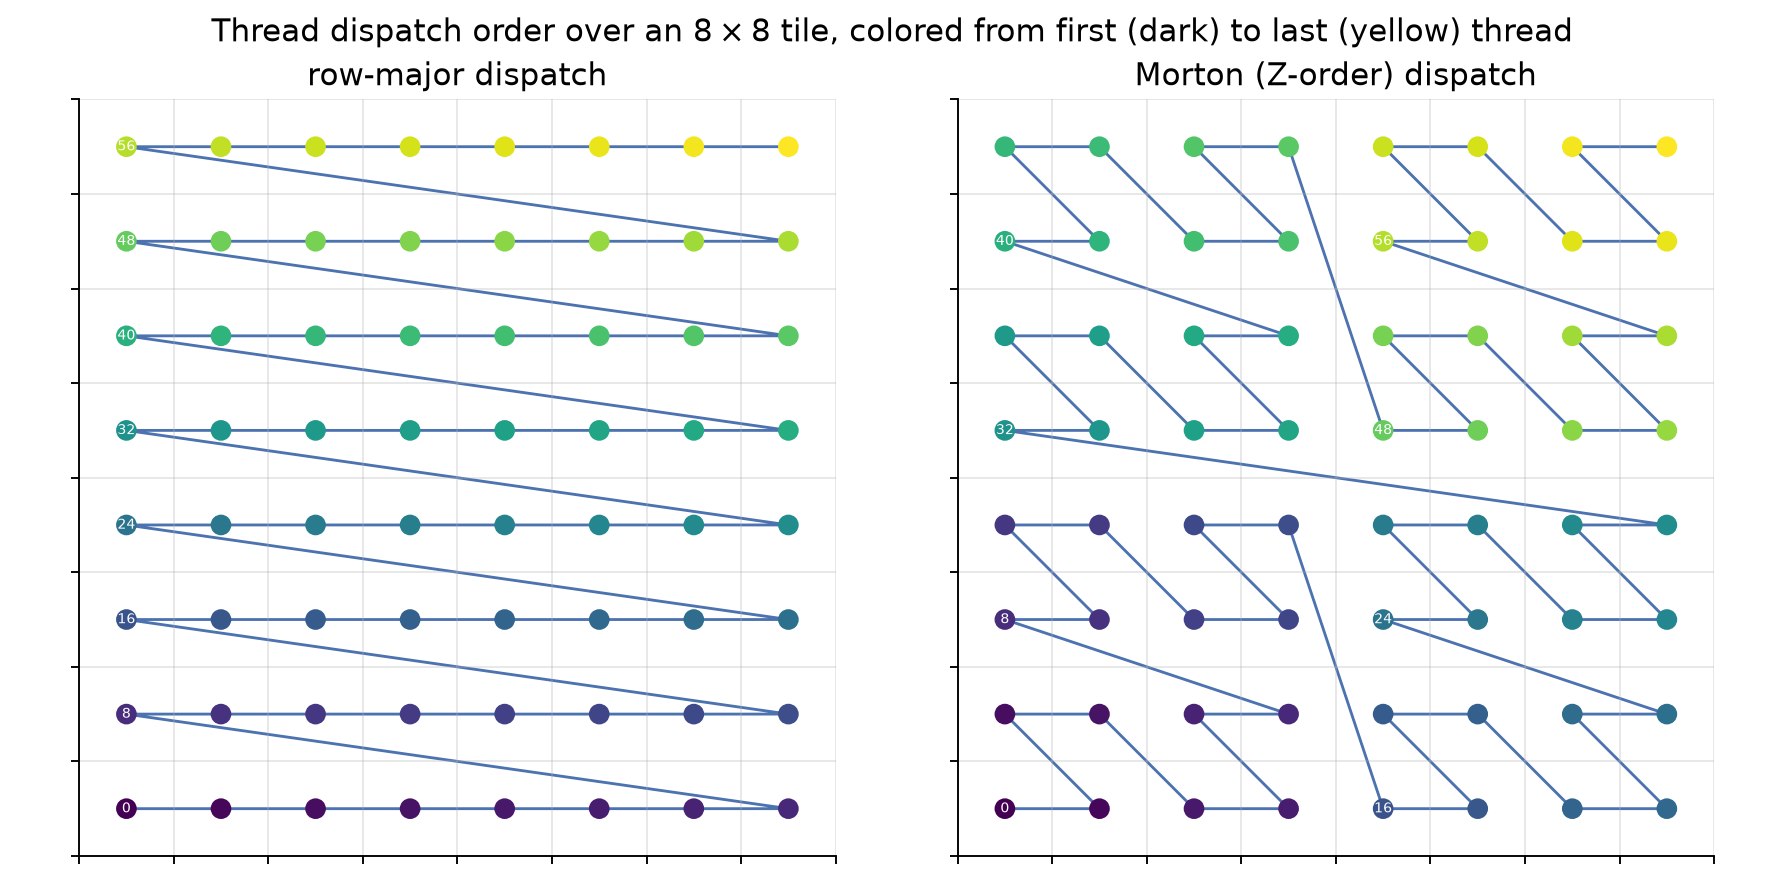
\includegraphics[width=\textwidth]{figures/gpu-traversal-order.png}
  \caption{Thread dispatch order over an $8\times8$ tile. Row major order jumps back across the
  full tile width at the end of every row, so consecutive thread indices land far apart in $y$ at
  those boundaries. Morton order keeps consecutive indices inside the same $2\times2$ or $4\times4$
  quadrant far more often, the locality property Section~\ref{sec:gpu-traversal} argues should help
  a warp's iteration counts stay uniform.}
  \label{fig:gpu-traversal-order}
\end{figure}

Measured directly, that reasoning does not pay off on this hardware. A same process, paired
comparison against a plain row major grid, using the same kernel math dispatched through the
scheduler's tiled entry point instead, shows the Morton launch issuing just over twice as many
threads as there are pixels, $4{,}194{,}304$ against $2{,}073{,}600$ for a $1920\times1080$ frame,
since padding to a square roughly doubles the grid. The median cost across seven repeated runs
was about $+1.9\%$, with two of the seven runs actually favoring the Morton launch. That is
indistinguishable from noise. The excess threads land in one contiguous region past the frame's
true edge, so whole blocks retire immediately rather than doing any wasted per pixel work, which is
why doubling the launched thread count costs next to nothing either way. The padding is nearly
free, but so, on this measurement, is the ordering it was meant to enable. This is the same verdict
Section~\ref{sec:traversal-locality} reached testing a Hilbert curve on the CPU, a space filling
traversal order chosen on locality grounds, tested directly against the plain alternative, and
found not to move the number on the hardware actually measured.

The heterogeneous scheduler does not use the Morton path at all for the tiles it sends to the GPU.
It dispatches through a tiled kernel instead, one block per tile selected by the block's $z$ index,
each thread bounds checked against its own tile's width and height. A second variant of that tiled
kernel additionally carries a destination offset per tile, for writing into one densely packed
output buffer rather than each tile's own position in a full frame, used when the scheduler hands
the GPU a scattered subset of the image rather than a contiguous region of it
(Chapter~\ref{ch:scheduler}).

Underneath either traversal order, both backends write into the same kind of buffer, a flat,
row major array of one \kod{f32} per pixel holding the raw, possibly fractional escape time value
from Equation~\ref{eq:smooth-coloring}, not a color, at $4$ bytes per pixel. That is
$8.29\,\mathrm{MB}$ for the $1920\times1080$ frame measured throughout this chapter. Turning that
into a displayed image, histogram, cumulative distribution, and palette lookup, is a separate pass
over the same buffer, run as its own pair of kernels on the CUDA side, mirroring the two stage
render then colorize split the CPU pipeline already uses.

Sections~\ref{sec:webgpu} and~\ref{sec:cuda} both measured host readback at $80$ to $90\%$ of total
frame time, an order of magnitude more than the traversal choices in this section moved the number
by. The hybrid scheduler in Chapter~\ref{ch:scheduler} is built around that readback cost.

\chapter{Hybrid CPU and GPU Scheduler}
\label{ch:scheduler}

\section{Motivation \& Design}
\label{sec:scheduler-motivation}

Chapter~\ref{ch:gpu} ended on a single number. Host readback is $80$ to $90\%$
of a GPU frame, on both backends, and no kernel level optimization touches that share. Nothing
in this thesis's rendering algorithms shrinks that
cost, because it has nothing to do with the algorithm. It is simply the price of moving a finished
buffer across PCIe. What a per pixel algorithm \emph{can} change is which device computes that
buffer's pixels in the first place, and the two devices are not equally good at every pixel.
GPU threads execute in warps of $32$, in lockstep, so if one thread in a warp reaches the
iteration cap while another escapes after ten iterations, the whole warp keeps running until
its slowest member finishes. That is the same masked lane cost the SIMD kernels in
Section~\ref{sec:simd} pay at a width of eight, except a stalled GPU warp cannot be handed other
work mid flight the way an idle CPU core can. A CPU core has no such constraint. Each of its
threads runs its own pixels independently, so a chaotic, high iteration count region costs that
core time proportional to its own pixels and nothing more. Regions of the image near the set's
boundary, where neighbouring pixels' escape counts diverge sharply, are therefore cheap on a CPU
and comparatively expensive on a GPU. Uniform regions, deep in the set or far outside it, are
cheap on both, because a GPU's lockstep execution has no divergence penalty left to pay there. The
scheduler in this chapter exploits exactly that asymmetry. It routes each part of the image to
whichever device pays less for \emph{that} part, in the spirit of adaptive heterogeneous mapping
across CPU and GPU \cite{luk2009qilin}, rather than rendering the whole frame on one device or
splitting it by a fixed rule that ignores content.

The design has four moving pieces. First, before any pixel is rendered, the frame is decomposed into tiles and each tile is classified as
suitable for the GPU or suitable for the CPU, cheaply, by sampling only its four corners
(Section~\ref{sec:tile-decomposition}). Second, that classification is turned into actual work.
GPU classified tiles are dispatched to the GPU while a pool of CPU workers concurrently drains
the CPU classified tiles from a shared queue, the two running concurrently for the whole frame
rather than one waiting on the other (Section~\ref{sec:work-distribution}). Third, a
split decided
before either device has rendered a single pixel cannot know either device's load in real time, so a
fraction of the GPU's tiles are held back as work any idle CPU core can steal once its own queue
is empty, correcting for a temporarily slow GPU within the same frame
(Section~\ref{sec:work-distribution}). Fourth, correcting only within a frame is not enough if
one device is \emph{consistently} faster or slower than the classifier's static threshold
assumes, since interactive rendering renders the frame again on every pan and zoom. Each frame's own measured
GPU and CPU time therefore feeds a PI controller that retunes the classifier's threshold for the next frame,
closing the loop across frames rather than within one (Section~\ref{sec:load-balancing}).

\begin{figure}[H]
  \centering
  \resizebox{\textwidth}{!}{%
  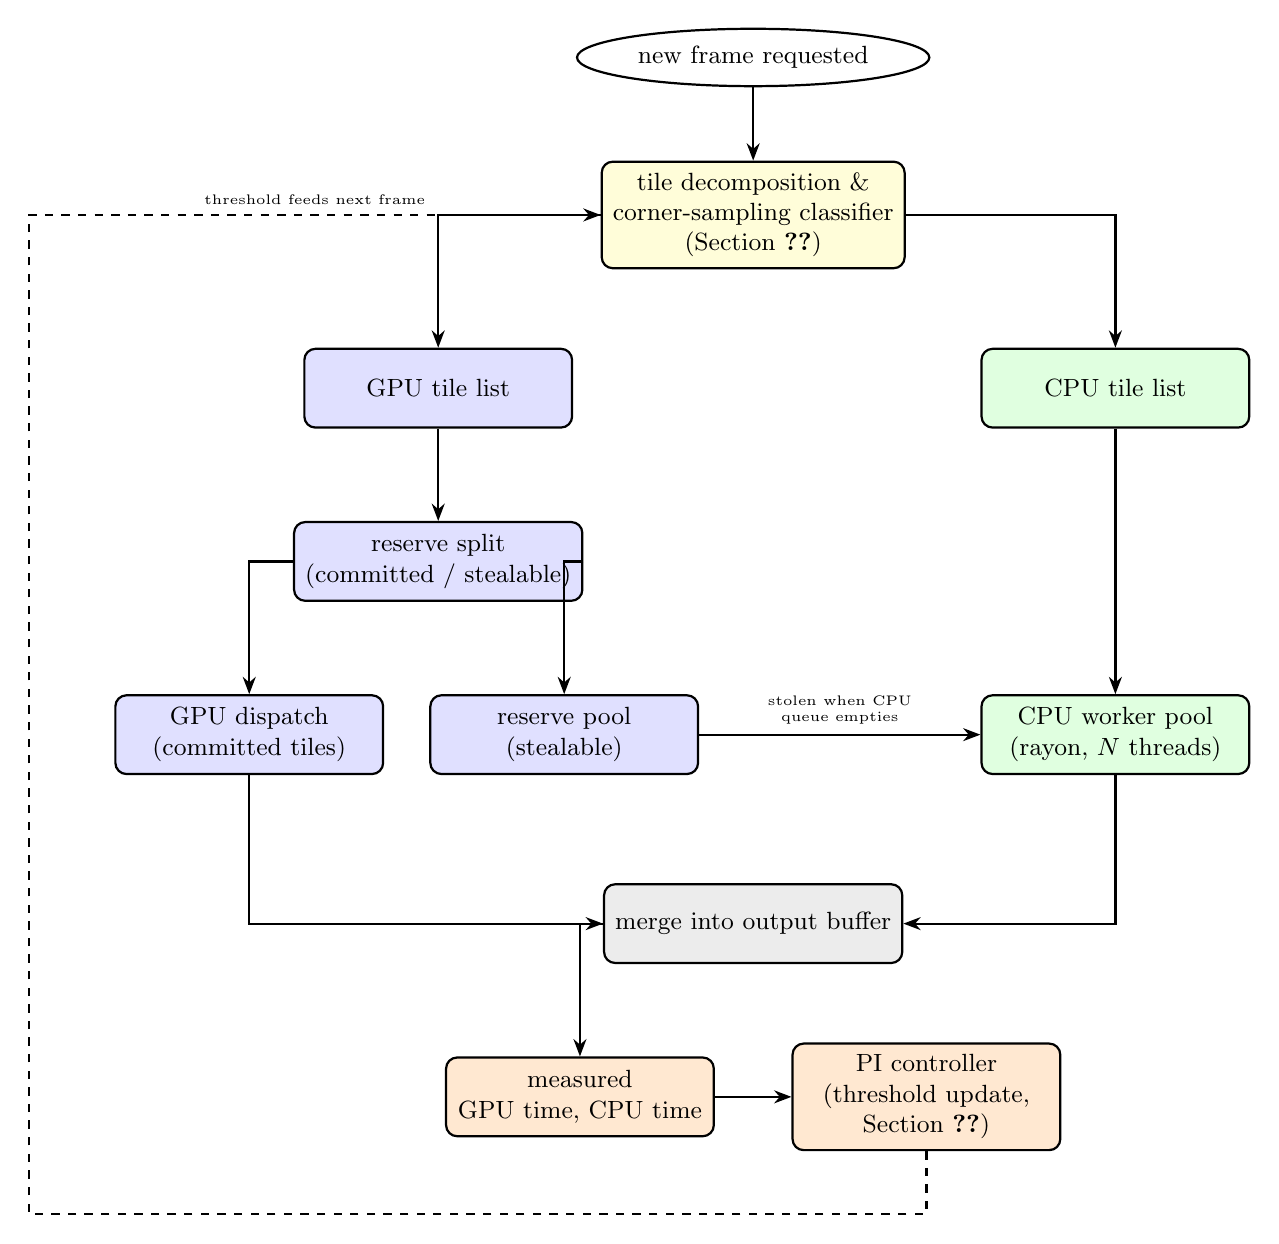
\begin{tikzpicture}[
    font=\small,
    box/.style={rectangle, rounded corners, draw=black, thick, minimum width=3.4cm,
      minimum height=1cm, align=center, inner sep=4pt},
    classify/.style={box, fill=yellow!15},
    gpubox/.style={box, fill=blue!12},
    cpubox/.style={box, fill=green!12},
    mergebox/.style={box, fill=gray!15},
    ctrlbox/.style={box, fill=orange!18},
    startbox/.style={ellipse, draw=black, thick, fill=white, minimum width=2.6cm,
      minimum height=0.7cm, align=center},
    arrow/.style={-{Stealth[length=2.2mm]}, thick},
  ]
  \node[startbox]  (start)       at (0,0)       {new frame requested};
  \node[classify]  (classify)    at (0,-2)      {tile decomposition \&\\corner-sampling classifier\\(Section~\ref{sec:tile-decomposition})};

  \node[gpubox]    (gputiles)    at (-4,-4.2)   {GPU tile list};
  \node[cpubox]    (cputiles)    at (4.6,-4.2)  {CPU tile list};

  \node[gpubox]    (split)       at (-4,-6.4)   {reserve split\\(committed / stealable)};
  \node[gpubox]    (gpudispatch) at (-6.4,-8.6) {GPU dispatch\\(committed tiles)};
  \node[gpubox]    (reserve)     at (-2.4,-8.6) {reserve pool\\(stealable)};
  \node[cpubox]    (cpuworkers)  at (4.6,-8.6)  {CPU worker pool\\(rayon, $N$ threads)};

  \node[mergebox]  (merge)       at (0,-11.0)   {merge into output buffer};

  \node[ctrlbox]   (measure)     at (-2.2,-13.2) {measured\\GPU time, CPU time};
  \node[ctrlbox]   (pi)          at (2.2,-13.2)  {PI controller\\(threshold update,\\Section~\ref{sec:load-balancing})};

  \draw[arrow] (start) -- (classify);
  \draw[arrow] (classify) -| (gputiles);
  \draw[arrow] (classify) -| (cputiles);
  \draw[arrow] (gputiles) -- (split);
  \draw[arrow] (split) -| (gpudispatch);
  \draw[arrow] (split) -| (reserve);
  \draw[arrow] (cputiles) -- (cpuworkers);
  \draw[arrow] (reserve) -- (cpuworkers)
    node[midway, above, font=\tiny, align=center] {stolen when CPU\\queue empties};
  \draw[arrow] (gpudispatch) |- (merge);
  \draw[arrow] (cpuworkers) |- (merge);
  \draw[arrow] (merge) -| (measure);
  \draw[arrow] (measure) -- (pi);
  \draw[arrow, dashed] (pi.south) -- ++(0,-0.8) -| (-9.2,-2) -- (classify.west)
    node[midway, above, font=\tiny, align=left] {threshold feeds next frame};
  \end{tikzpicture}%
  }
  \caption{The hybrid scheduler's per frame data flow. Yellow is the classifier, blue is the GPU
  path, green is the CPU path, gray is the merge step, and orange is the cross frame feedback loop
  that closes through the PI controller. The dashed arrow is the only edge that crosses a frame
  boundary, every solid edge happens within the frame currently being rendered.}
  \label{fig:scheduler-diagram}
\end{figure}

\section{Tile Decomposition and Classification}
\label{sec:tile-decomposition}

The classifier's job is to decide, for a region of the frame no pixel of which has been rendered
yet, whether that region belongs on the GPU or the CPU, and to do so without spending anywhere
near as much time as actually rendering it would. It works by corner sampling. The escape time
kernel is evaluated at a tile's four corners only, and how much those four values disagree serves
as a proxy for how divergent the pixels inside are likely to be. The frame is first covered by a
row major grid of equally sized cells ($128 \times 128$ pixels by default), classified
independently and in parallel, since one cell's classification touches no shared
state and depends on no other cell's outcome.

Within a cell, the four corner values give a normalized spread,
\begin{equation}
  \label{eq:corner-spread}
  s = \frac{\max(i_1,i_2,i_3,i_4) - \min(i_1,i_2,i_3,i_4)}{N},
\end{equation}
where $i_1,\dots,i_4$ are the four corners' escape time iteration counts and $N$ is the iteration
cap, comparable across different iteration caps since it is a fraction of the iteration budget
rather than a raw iteration count. If $s$ falls below a threshold, the tile is
classified GPU, since its corners agree closely enough that the pixels between them are assumed
uniform. That is the same locality assumption Mariani-Silver's border test
(Section~\ref{sec:mariani-silver}) makes about a rectangle's interior, applied here to route work
between devices instead of to skip it outright. If $s$ is at or above threshold, the tile
is bisected along its longer axis, the same split by longer axis Mariani-Silver's border test uses,
into two tiles that are each classified recursively, reusing the two corner samples on the
shared edge from the parent and evaluating only the two genuinely new corners the split creates,
rather than resampling all four for each half. Recursion bottoms out at a minimum tile size
($16 \times 16$ pixels by default). A tile that small is classified CPU regardless of its spread,
since subdividing further stops paying for itself no matter how divergent the tile still looks.
The threshold itself is not fixed. Section~\ref{sec:load-balancing} covers where it comes from.

The classifier's output is two separate lists of tile rectangles, one bound for the GPU and one
bound for the CPU, that Section~\ref{sec:work-distribution} dispatches from directly. Measured
directly, this whole pass costs $0.03$ to $0.32\,\mathrm{ms}$ across a shallow to moderate zoom
range, negligible next to the frame times it precedes, which run several milliseconds each.
Sampling only four corners per tile, rather than every pixel, keeps the cost of deciding where to
render small relative to the cost of actually rendering. The split it produces also tracks scene
content rather than applying some fixed ratio. On this thesis's benchmark scene, the CPU's share
of pixels rises from about $3\%$ at zoom $1$ to about $14\%$ at zoom $100$, as the set's boundary,
the only region divergent enough to fail the corner test, comes to fill more of the frame.

\begin{figure}[H]
  \centering
  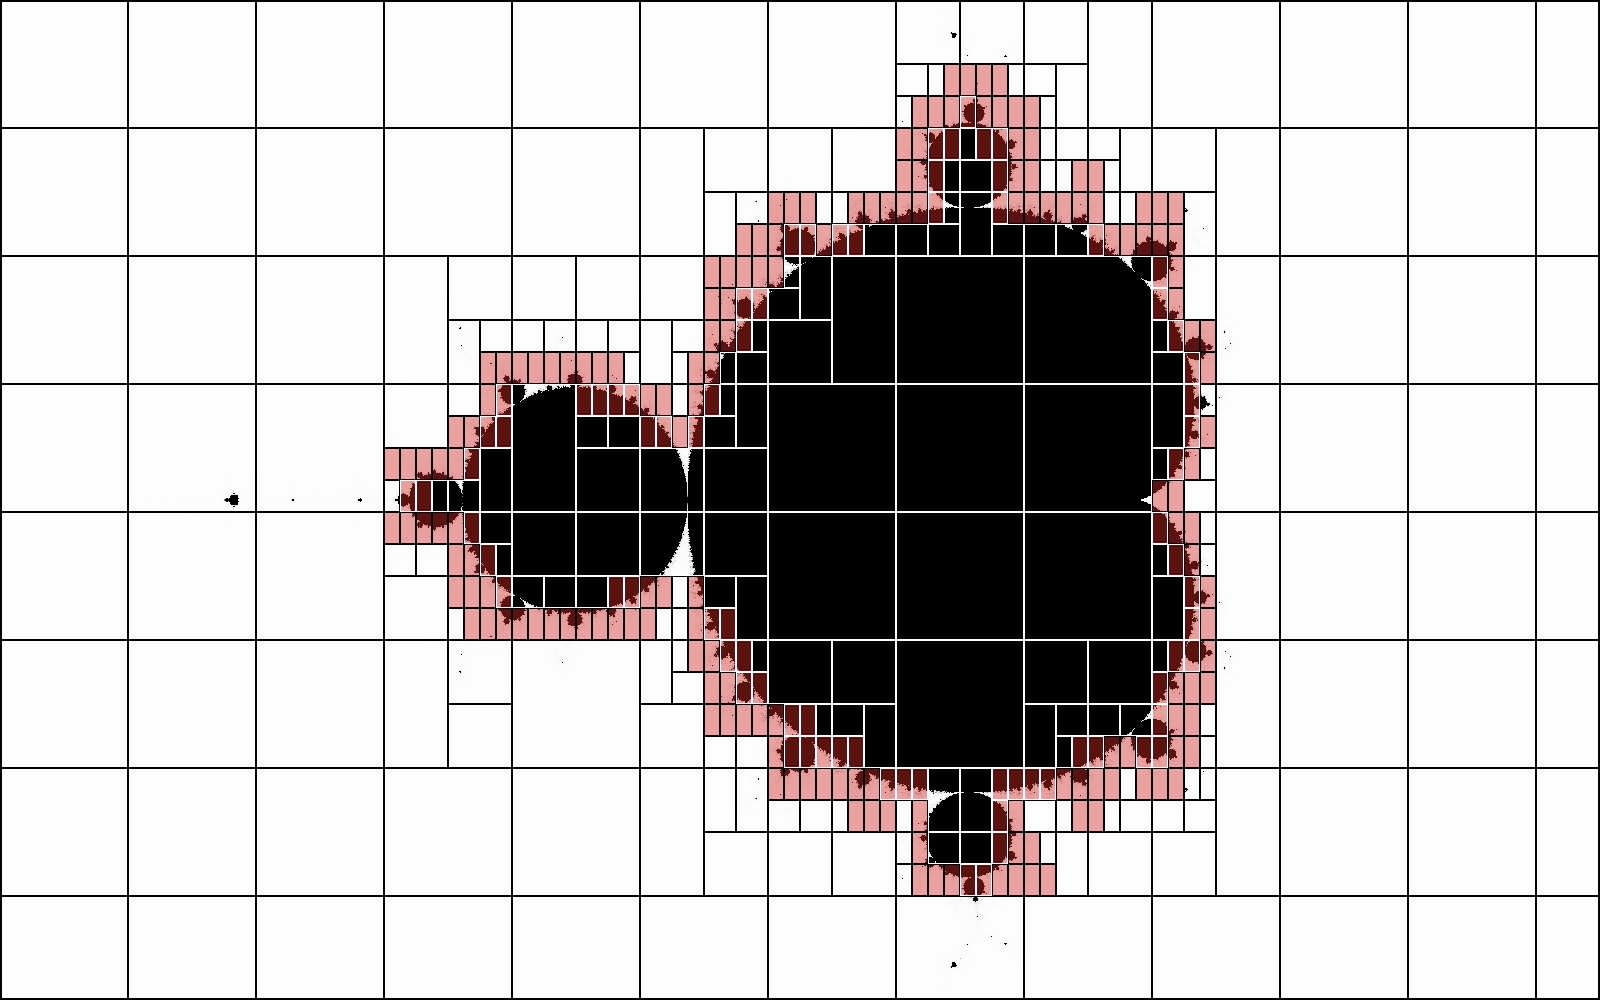
\includegraphics[width=0.8\textwidth]{figures/sched-tiling.png}
  \caption{The classifier's tile partition over a full frame Mandelbrot render.
  GPU classified tiles are left untinted. CPU classified tiles are shaded red.}
  \label{fig:sched-tiling}
\end{figure}

Figure~\ref{fig:sched-tiling} makes that concentration visible. The CPU tiles form a thin band
that follows the boundary's own shape rather than a solid mass, and recursion pushes deepest
exactly where that shape is least like a straight line. The cusps where the main cardioid meets
its attendant bulbs stand out as small clusters of minimum size tiles within the wider band. That
is the same effect behind the $3\%$ to $14\%$ CPU share reported above. However finely the
boundary folds at scales below a single pixel, the tile grid can only ever resolve it down to
minimum tile resolution, so the CPU's share stays tied to how much of the visible frame the
boundary curve passes through, not to how complex that curve actually is.

\section{Work Distribution \& Synchronization}
\label{sec:work-distribution}

The classifier's GPU list is not committed to the GPU in full. A trailing fraction of it, $20\%$
by default, is split off into a separate reserve pool instead, and the remainder, the committed
tiles, is what actually gets dispatched to the GPU immediately. Both the reserve pool and the
CPU list, now a work queue of its own, are shared, contended state that any CPU worker thread can
draw from.

One worker thread runs per available CPU core, and each worker loops. It claims a tile from its
own CPU queue first, and only reaches into the reserve pool once that queue is empty, so
GPU reserved work is touched only after a worker's own designated share is exhausted. While those
workers run concurrently, the GPU is dispatched on the committed tiles in one
batch, so neither device waits on the other for the bulk of the frame. Once that dispatch
returns, the scheduler checks how many tiles are still unclaimed in the reserve pool. If at least
$64$ remain, the CPU workers evidently have not gotten to them yet, still busy with their own
queue, so it is worth one more GPU dispatch to finish the remainder rather than wait on the CPU
to eventually drain it. Otherwise the remainder is small enough that a second GPU launch's own
overhead would not be worth paying, and it is simply left for CPU workers to keep stealing. The
GPU readback that follows copies the entire frame buffer regardless of which fraction the GPU
actually rendered, since shrinking that copy would require the GPU's share to be one contiguous
row range rather than a scattered set of tiles.

Once every CPU worker and the GPU dispatch have both finished, each device's rendered tiles are
copied into their true position in a shared output buffer. No per pixel or per tile lock is
needed during rendering itself, only the brief moment a worker claims a tile from a queue. The
tiles a GPU and a CPU worker render are always disjoint, so the merge step that follows has no
contention to resolve.

\section{Adaptive Load Balancing with a PI Controller}
\label{sec:load-balancing}

The classifier's threshold (Section~\ref{sec:tile-decomposition}) is a proxy for how divergent a
tile's interior is likely to be, not a direct measurement of which device renders that tile
faster, and the right proxy value depends on scene content and on the two devices' relative load
in ways nothing upstream of rendering can know in advance. A feedback controller instead closes
the loop from the outside. It observes each frame's actual measured GPU and CPU wall clock time
and nudges the threshold so the two stay balanced on the next frame.

The controller tracks one signed error per frame, $\mathrm{error} = t_{\mathrm{gpu}} -
t_{\mathrm{cpu}}$, the difference between that frame's measured GPU and CPU render time, and
updates the threshold as
\begin{equation}
  \label{eq:pi-controller}
  \mathrm{threshold} \mathrel{-}= K_P \cdot \mathrm{error} + K_I \cdot \overline{\mathrm{error}},
\end{equation}
with $K_P = 0.0005$ and $K_I = 0.00005$, then clamps the result to $[0.001, 0.5]$. A positive
error means the GPU was slower than the CPU that frame, and Equation~\ref{eq:pi-controller}
responds by lowering the threshold. Since the classifier's own test is $\mathrm{spread} <
\mathrm{threshold}$, a lower threshold is a stricter uniformity requirement, so fewer tiles pass
it and more are routed to the CPU on the next frame, relieving the device that was behind. A
negative error drives the threshold the other way. The proportional term alone reacts to the
current frame only and would leave a steady state bias uncorrected if one device is
\emph{consistently} faster rather than just noisily so from frame to frame. The integral term
$\overline{\mathrm{error}}$, a moving average over the last $16$ frames rather than an unbounded
running sum, corrects that residual bias while still letting a single
noisy frame's influence age out after sixteen updates instead of persisting forever. The
proportional gain is ten times the integral gain, so the controller reacts fastest to the
frame it just measured and leans on the integral term only for what that alone does not fix. The
$[0.001, 0.5]$ clamp keeps a large, sustained imbalance, such as a GPU driver stall, from driving
the threshold to an extreme where the classifier collapses to routing everything to one device
regardless of content, which would throw away the awareness of content Section~\ref{sec:tile-decomposition}
was built to provide in the first place.

\begin{figure}[H]
  \centering
  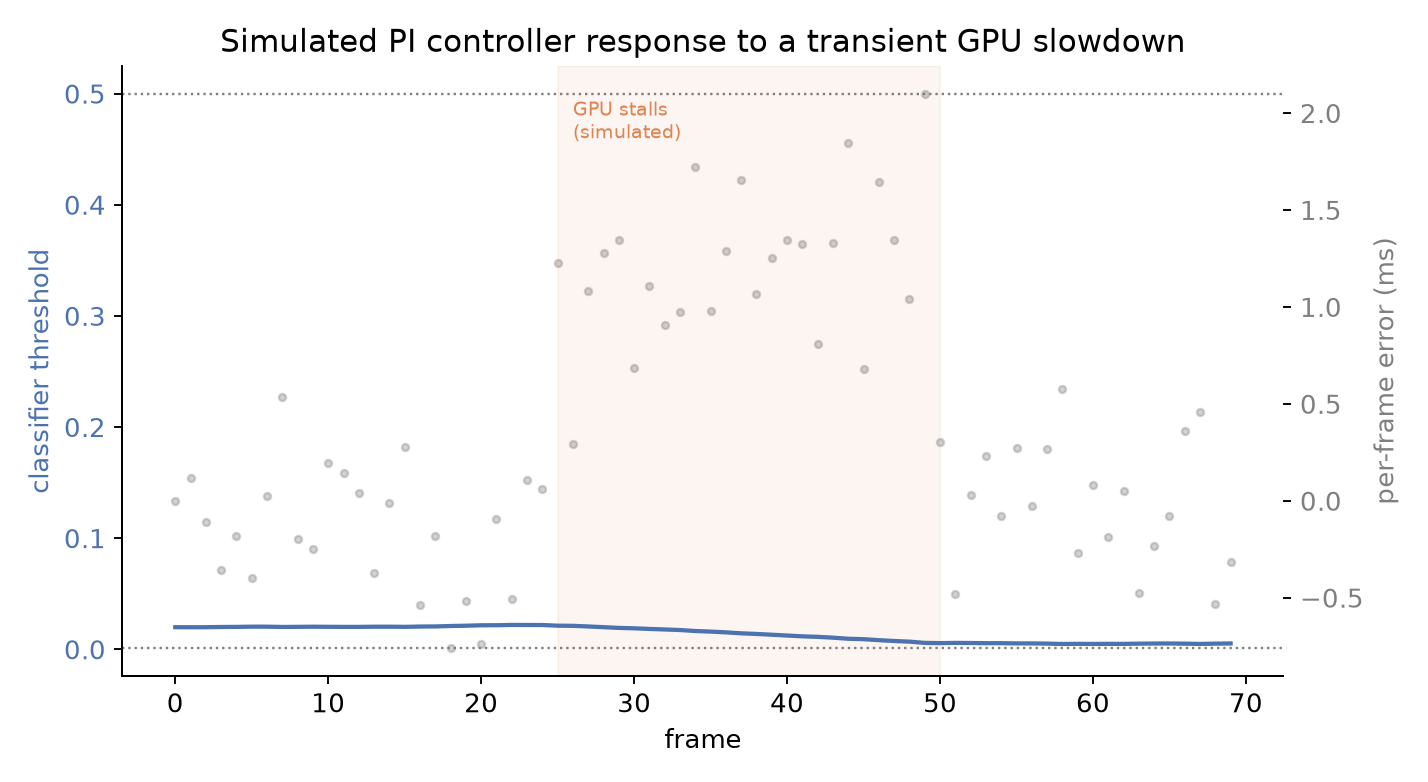
\includegraphics[width=0.75\textwidth]{figures/pi-controller-response.png}
  \caption{Equation~\ref{eq:pi-controller} simulated over $70$ synthetic frames, with a transient
  GPU stall injected between frames $25$ and $50$. The threshold falls while the stall lasts,
  routing more of the frame to the CPU, and the sixteen frame integral window keeps pulling it down
  for a few frames after the stall ends before the proportional term settles on zero mean noise
  again. This run happens to reach the $0.001$ floor, illustrating exactly the case the clamp above
  is there to bound.}
  \label{fig:pi-controller-response}
\end{figure}

Because interactive rendering renders the frame again on every pan and zoom, this feedback runs continuously
rather than as a one time calibration step. The update runs at the end of
every heterogeneous render, and the threshold it leaves behind is exactly what
Section~\ref{sec:tile-decomposition}'s classifier reads at the start of the very next one. Taken
together with the stealing within a frame from Section~\ref{sec:work-distribution}, the scheduler
corrects for load imbalance on two timescales at once. Stealing absorbs a GPU that runs behind
within a single frame, and the controller absorbs a GPU that runs behind \emph{across} frames by
reshaping the classification itself. Chapter~\ref{ch:results} measures how much of the readback
cost this chapter opened with that combination actually recovers, and where the two devices are
close enough in speed for the correction to matter at all.

\chapter{Experimental Methodology}
\label{ch:methodology}

Chapter~\ref{ch:results} reports frame time, throughput, and scaling
behaviour for every backend built in Chapters~\ref{ch:algorithms},
\ref{ch:gpu}, and~\ref{ch:scheduler}. This chapter defines the conditions
those numbers were produced under. Section~\ref{sec:technology-stack}
covers the software stack and how it is configured and measured.
Section~\ref{sec:hardware} covers the machine. Section~\ref{sec:benchmarks}
covers the fractals, resolutions, and viewports exercised, and
Section~\ref{sec:metrics} covers the quantities reported.

\section{Technology Stack}
\label{sec:technology-stack}

\subsection{Rust}
\label{sec:rust}

Rust is a compiled systems language with no garbage collector. Memory
safety and freedom from data races are enforced at compile time through
ownership and borrow checking, not a runtime collector. That guarantee
matters for a renderer whose reported unit is millisecond frame time. A
garbage collected implementation would need every measurement split into
collection pauses and algorithmic cost before a single number in
Chapter~\ref{ch:results} meant anything, and this renderer has no such
split to make. The compiler lowers to native code through LLVM, so generic
and iterator based Rust compiles to the same machine code as an equivalent
hand written loop. \kod{unsafe} blocks, used only for CUDA driver calls,
are the sole escape from the compiler's checks.

The project targets the 2024 edition and is built through two compile time
configurations, applied uniformly to every number in this thesis.
\begin{itemize}
  \item the release profile, \kod{opt-level = 3}, \kod{lto = "thin"},
  thin link time optimization across the whole dependency graph, and
  \kod{codegen-units = 1}, one codegen unit, trading compile time for the
  optimizer's full visibility into the program. No measurement in this
  thesis comes from a debug build, which is an order of magnitude slower
  and not a usable baseline, and
  \item \kod{-C target-cpu=native}, set via \kod{rustflags}, letting the
  compiler target every instruction set the reference machine's CPU
  (Section~\ref{sec:hardware}) actually exposes, including the AVX2
  instructions the \kod{f32x8}/\kod{f64x4} SIMD kernels compile down to.
  A conservative default target would not emit those instructions at all.
\end{itemize}

Four crates carry the CPU side implementation. This states what each one
is used \emph{for}, not how, since Section~\ref{sec:baseline-scalar} and
Section~\ref{sec:simd} already cover the kernels themselves.
\begin{itemize}
  \item \kod{rayon}, the work stealing thread pool behind every CPU kernel,
  scalar and SIMD alike,
  \item \kod{wide}, the portable \kod{f64x4}/\kod{f32x8} SIMD vector types,
  \item \kod{num-complex}, the complex number arithmetic the escape time
  kernels iterate, and
  \item \kod{image}, writing rendered frames to PNG for output
  verification.
\end{itemize}

\subsection{GPU Technologies}
\label{sec:gpu-tech}

Two GPU technologies back the two GPU kernels compared in this thesis, and
they differ in what they let this thesis control at compile time. WebGPU is
a portable compute and graphics API, standardized independently of any one
vendor. A driver maps it onto whichever native API a platform exposes,
Vulkan on the reference machine. Its shaders are written in WGSL and
compiled at runtime by the driver, so one kernel source runs unmodified on
any WebGPU capable device, at the cost of no compile time control over the
machine code the driver's own compiler ultimately produces. This thesis
reaches WebGPU through \kod{wgpu} (version~22), the Rust implementation
also used by Firefox and Deno.

CUDA is NVIDIA's proprietary compute platform. Kernels are
compiled ahead of time with \kod{nvcc} into PTX, NVIDIA's stable
intermediate representation, embedded into the compiled binary so nothing
needs compiling at runtime. Five flags configure that compilation, applied
identically to every CUDA kernel in this thesis.
\begin{itemize}
  \item \kod{--gpu-architecture=sm\_86}, targeting the Ampere generation of
  the reference GPU (Section~\ref{sec:hardware}) directly, rather than a
  generic target the driver would have to translate at load time,
  \item \kod{-O3}, \kod{nvcc}'s highest optimization level,
  \item \kod{--ftz=false}, keeping denormalized floats alive, needed for
  the smooth coloring formula's accuracy near the escape threshold,
  \item \kod{--prec-div=true}, full precision division, and
  \item \kod{--fmad=false}, disabling fused multiply add contraction so
  CUDA's arithmetic rounds exactly like the CPU kernels' does, at a
  measured cost under $1\%$ of kernel throughput once other precision
  costs are removed (Section~\ref{sec:cuda}).
\end{itemize}
This thesis reaches CUDA~12 through \kod{cudarc}, a Rust binding to the
CUDA driver API.

\subsection{Benchmarking Technology}
\label{sec:benchmarking-tech}

Three tools measure the renderer, each suited to a different purpose.
\begin{itemize}
  \item \kod{criterion}, a statistical benchmarking crate, runs the primary
  suite (\kod{fractal\_bench}). Each group gets a two second warm up,
  discarded, then five seconds of measurement, and reports a mean with a
  $95\%$ confidence interval rather than one sample. Repeated runs of a
  nominally identical kernel have disagreed by more than $50\%$ within a
  single \kod{criterion} invocation.
  \item \kod{bench\_runner}, a purpose built binary that renders one fixed
  configuration deterministically, for pairing with \kod{perf stat} or for
  emitting machine readable JSON, and
  \item a set of standalone probe binaries (\kod{gpu\_probe},
  \kod{ptx\_variants}, \kod{sched\_probe}, \kod{sched\_overhead},
  \kod{sched\_deepzoom}, \kod{tiled\_dispatch\_probe}, \kod{adapters}),
  each isolating one phase or one hypothesis that a single frame time
  number cannot separate on its own, for example kernel time from host
  readback time, one compiler flag's effect from another's, or scheduler
  overhead from scheduler decision quality.
\end{itemize}
\kod{perf stat} supplies CPU cache and branch counters, NVIDIA Nsight
Compute supplies GPU occupancy and warp efficiency counters, and RAPL
package energy counters together with \kod{nvidia-smi}'s power draw supply
the energy figures in Section~\ref{sec:scaling-energy}.

The four existing renderers surveyed in Section~\ref{sec:related-work}
share none of this tooling. Each was instrumented with an equivalent
two layer harness for this thesis, a Google Benchmark based
\kod{criterion\_bench} target and a \kod{bench\_runner} CLI call that
project's own compiled kernel directly, so all five renderers run from one
command line and produce comparable JSON. Each renderer's own threading
model is measured as built, not normalized to \kod{rayon}'s pool. The
comparison targets algorithmic throughput per pixel actually computed, so
any shortcut a project uses to avoid computing a pixel outright, such as
XaoS's boundary tracing or FractalNow's quad interpolation, is disabled.
Both substitute interpolation for computation on part of the image, which
would measure how well a project guesses rather than how fast its kernel
runs.

\section{Hardware}
\label{sec:hardware}

All measurements in this thesis, referred to throughout as the reference
machine, come from one laptop, built around the following.
\begin{itemize}
  \item an AMD Ryzen~7 5800H CPU, eight Zen~3 cores, sixteen threads via
  two way SMT,
  \item an NVIDIA GeForce RTX 3050 Laptop GPU, Ampere (\kod{sm\_86}), CUDA
  12.0, driver 580.173.02, PCIe~3.0 x8 ($8\,\mathrm{GB/s}$ theoretical), and
  \item an integrated AMD Radeon Vega GPU, code name Renoir.
\end{itemize}

Figure~\ref{fig:hardware-topology} lays out how these components actually
connect. The Ryzen die carries the Radeon Vega integrated GPU on package,
so both share the same dual channel DDR4 system RAM through one on die
memory controller, with no PCIe transfer between them at all. The RTX
3050 is a separate, discrete part reached only over PCIe~3.0 x8, with its
own dedicated GDDR6 VRAM the CPU cannot address directly, the link
Section~\ref{sec:gpu-traversal} and Chapter~\ref{ch:scheduler} spend so
much of this thesis working around the cost of.

\begin{figure}[H]
  \centering
  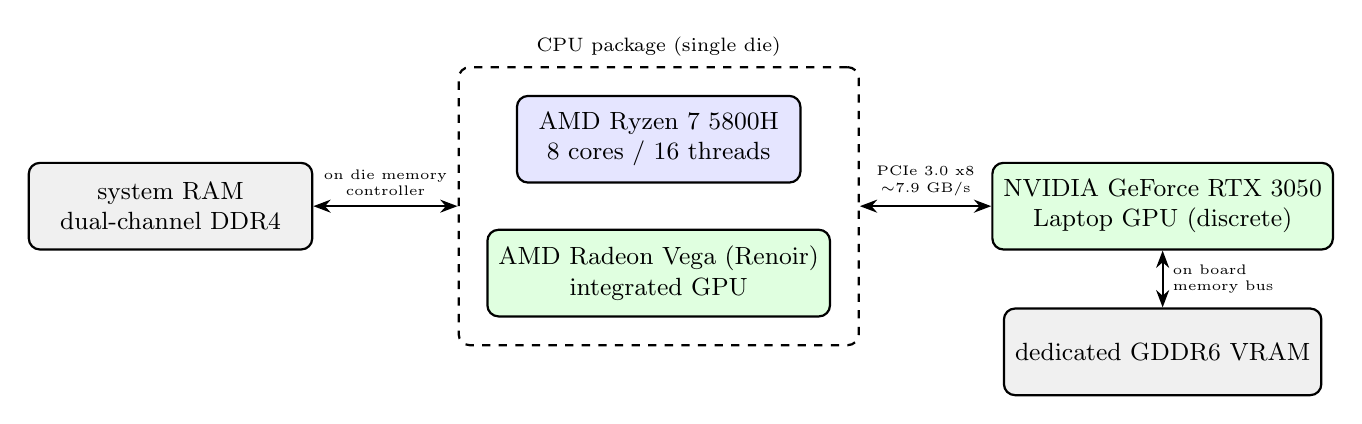
\begin{tikzpicture}[
    font=\small,
    comp/.style={rectangle, rounded corners, draw=black, thick, minimum width=3.6cm,
      minimum height=1.1cm, align=center, inner sep=4pt, fill=blue!10},
    gpucomp/.style={comp, fill=green!12},
    memcomp/.style={comp, fill=gray!12},
    pkg/.style={rectangle, rounded corners, draw=black, thick, dashed, inner sep=10pt},
    arrow/.style={{Stealth[length=2.2mm]}-{Stealth[length=2.2mm]}, thick},
  ]
  \node[comp]     (cpu)  at (0,0)   {AMD Ryzen~7 5800H\\8 cores / 16 threads};
  \node[gpucomp]  (igpu) at (0,-1.7) {AMD Radeon Vega (Renoir)\\integrated GPU};

  \node[pkg, fit=(cpu)(igpu), label={[font=\scriptsize]above:CPU package (single die)}] (pkgbox) {};

  \node[memcomp]  (ram)  at (-6.2,-0.85) {system RAM\\dual-channel DDR4};

  \node[gpucomp]  (dgpu) at (6.4,-0.85) {NVIDIA GeForce RTX 3050\\Laptop GPU (discrete)};
  \node[memcomp, minimum width=3cm]  (vram) at (6.4,-2.7) {dedicated GDDR6 VRAM};

  \draw[arrow] (ram) -- (pkgbox.west|-ram)
    node[midway, above, font=\tiny, align=center] {on die memory\\controller};
  \draw[arrow] (pkgbox.east|-dgpu) -- (dgpu)
    node[midway, above, font=\tiny, align=center] {PCIe 3.0 x8\\$\sim$7.9 GB/s};
  \draw[arrow] (dgpu) -- (vram)
    node[midway, right, font=\tiny, align=left] {on board\\memory bus};
  \end{tikzpicture}
  \caption{The reference machine's component topology. The integrated GPU shares the CPU package
  and system RAM at no transfer cost. The discrete GPU is reachable only over PCIe, with its own
  separate VRAM.}
  \label{fig:hardware-topology}
\end{figure}

\kod{wgpu}'s adapter selection
falls back silently to the integrated GPU when no NVIDIA Vulkan driver is
installed, understating GPU readback cost, since the integrated part
shares memory with the CPU and pays no PCIe transfer at all. Every
benchmark session logs the selected adapter at startup, checked before its
numbers are used.

The reference machine is a laptop, not a dedicated bench machine, and is
thermally variable. Identical CPU or GPU benchmarks, run in separate
sessions with no code change between them, have moved $15$ to $30\%$ from
thermal state alone. Every ratio and speedup figure in
Chapter~\ref{ch:results} is computed within a single run. Absolute
millisecond figures carry that variance regardless.

\section{Benchmarks and Test Scenes}
\label{sec:benchmarks}

\subsection{Fractals, Resolutions, and Iteration Counts}
\label{sec:bench-resolutions}

The Mandelbrot set is this thesis's sole benchmark target. The renderer
also implements Julia, Newton, and Nova fractals on the same escape time
machinery, but every optimization in
Chapters~\ref{ch:algorithms} through~\ref{ch:scheduler}, the cardioid and
bulb tests, the distance estimate, the Mariani-Silver subdivision, and
the SIMD and GPU kernel work, was developed and measured against
Mandelbrot specifically, and that is what the rest of this thesis
reports.

The benchmark suite exercises Mandelbrot at three resolutions,
$800\times600$, $1920\times1080$, and $3840\times2160$, chosen to
confirm that a technique's benefit holds independently of frame size.
Unless a sweep states otherwise, \kod{max\_iter} is fixed at $1000$. The
one exception is a convergence check against the Mandelbrot set's area,
estimated in the literature at approximately $1.50659177$, which sweeps
\kod{max\_iter} itself, from $100$ to $20000$.

\subsection{Viewports}
\label{sec:bench-viewports}

Most benchmarks render the whole visible set from its natural center
($c=-0.5$, zoom $1$), mixing interior, boundary, and fast escaping pixels
in roughly the proportions an interactive session shows. Where a
technique's cost depends specifically on how much of the frame is
boundary rather than interior, the suite instead uses five fixed sample
points spanning the main cardioid, the largest bulb, a minibrot, and a
filament dense region, so a result cannot be an artifact of one
convenient view with little boundary in it.

\begin{figure}[H]
  \centering
  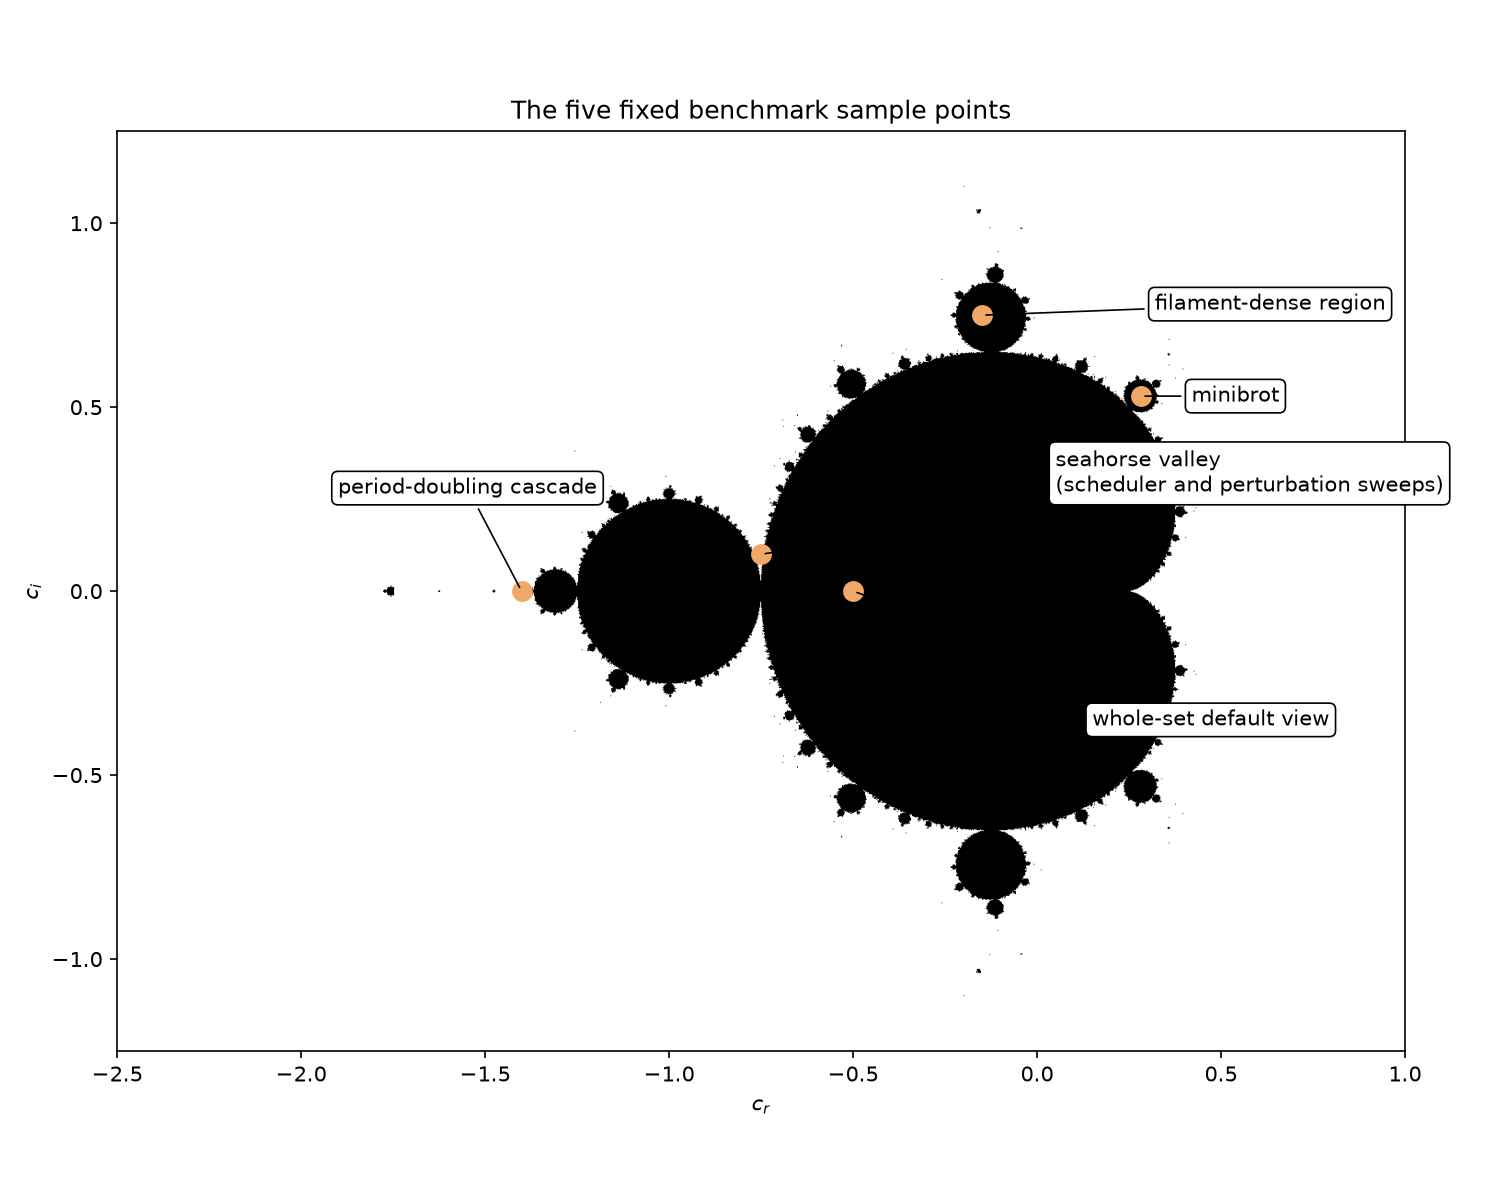
\includegraphics[width=0.75\textwidth]{figures/benchmark-viewport-map.png}
  \caption{The five fixed sample points, chosen to span a whole set view, a filament dense
  boundary region, a minibrot, and the period doubling cascade toward the Feigenbaum point along
  the negative real axis. The seahorse valley point doubles as the reference center for the zoom
  sweeps in Section~\ref{sec:bench-zoom-sweeps}.}
  \label{fig:benchmark-viewport-map}
\end{figure}

\subsection{Zoom Sweeps}
\label{sec:bench-zoom-sweeps}

Three sweeps probe zoom dependent behaviour. A shallow sweep (zoom $1$,
$10^2$, $10^4$) stays below the $10^6$ threshold where both CPU and GPU
kernels hand off from \kod{f32} to \kod{f64}. A deep sweep (zoom $10^4$ to
$10^{15}$) crosses that threshold, at a fixed seahorse valley reference
point ($c=-0.75+0.1i$) chosen because its boundary stays dense enough, at
every zoom level in the sweep, to give the tile classifier real work. A
third sweep (zoom $1$ to $10^{12}$, same reference point) evaluates
perturbation theory against plain \kod{f64}.

\subsection{Cross Renderer Comparison}
\label{sec:bench-cross-renderer}

The comparison against the four existing renderers is restricted to what
all five projects share, the Mandelbrot kernel, at matched
resolution, iteration count, and view, measured as raw per pixel
iteration time rather than full colored frames, since the renderers
differ in how much color mapping work is fused into that step.

\section{Metrics}
\label{sec:metrics}

\subsection{Frame Time and Throughput}
\label{sec:metrics-throughput}

Frame time is reported as \kod{criterion}'s sample mean with its
confidence interval. Throughput, pixels rendered per millisecond, comes
from the same measurement via \kod{criterion}'s element count facility
rather than being derived afterward. A flat throughput curve across
resolutions is this thesis's working definition of an embarrassingly
parallel kernel. A curve that bends indicates a cost scaling with frame
size rather than pixel count alone.

\subsection{Compute Efficiency}
\label{sec:metrics-gflops}

Cross kernel comparisons are additionally stated in GFLOPS, under one
fixed convention. Each iteration of the canonical $z = z^2 + c$ update
counts as eight floating point operations, with no credit for
fused multiply add contraction. The convention is a simplification, not a
literal instruction count, but applying it uniformly, to this renderer's
own kernels and to all four competitor projects, is what makes a GFLOPS
figure comparable across five independently written codebases.

\subsection{Precision Controlled Comparison}
\label{sec:metrics-precision}

Every reported speedup states the precision, \kod{f32} or \kod{f64}, both
sides ran at. Pairing a fast \kod{f32} GPU kernel against a slower
\kod{f64} CPU baseline inflates the apparent gain independently of either
device's real throughput, the effect Lee et al.\ document for CPU versus
GPU comparisons generally \cite{lee2010debunking}. Every GPU versus CPU
ratio in this thesis is reported at least twice, once against a naive
scalar baseline, and once against the CPU's own best available kernel at
matching precision.

\subsection{Parallel Scaling and Energy}
\label{sec:scaling-energy}

Thread scaling is reported as speedup and parallel efficiency relative to
that same renderer's own single threaded run, never across renderers,
since threading models differ structurally between projects. Energy
efficiency is reported separately from speed, as gigaflops per watt, from
RAPL package energy counters (CPU) and \kod{nvidia-smi} power draw (GPU)
over a sustained run, since a slower device is not necessarily a less
efficient one.

\subsection{Correctness and Microarchitectural Metrics}
\label{sec:correctness-metrics}

Two further metrics apply where the question is not about speed. Where an
optimization is expected to change performance only, never output,
correctness is checked as a per pixel difference count between kernel
variants. Zero differing pixels across the full frame is the bar any such
change must clear before its speed number is reported. Where a hypothesis
concerns GPU execution behaviour specifically, for instance whether
boundary heavy regions cause more warp divergence than uniform ones, warp
occupancy and warp efficiency, read directly from Nsight Compute, settle
it independently of whether the effect is large enough to move frame
time.

\chapter{Results and Discussion}
\label{ch:results}

This chapter presents the measurements the setup in
Chapter~\ref{ch:methodology} produces. Every figure comes from the
reference machine defined there, and every ratio quoted here follows the
precision controlled and within run comparison rules
Section~\ref{sec:metrics} sets out. Most figures in this chapter are
generated directly by this project's own \kod{aggregate\_bench.py}
tooling, described in Section~\ref{sec:technology-stack}, from a single
archived benchmark run rather than redrawn by hand, so a number that
looks slightly different from one already quoted in an earlier chapter is
run to run thermal variance, the kind Section~\ref{sec:hardware}
describes, not a contradiction. The chapter follows the order
Chapters~\ref{ch:algorithms} through~\ref{ch:scheduler} introduced the
underlying techniques in, the CPU baseline and SIMD first, then the two
GPU backends, the end to end pipeline, the hybrid scheduler, perturbation
theory, and finally the cross project and numerical validation results.
Two results carry more weight than the rest. Figure~\ref{fig:results-gpu-resolution}
in Section~\ref{sec:results-gpu} is the single measurement every earlier
optimization chapter feeds into, render throughput for every backend this
thesis built, side by side, and Section~\ref{sec:results-scheduler} is
where the hybrid scheduler, this thesis's central contribution, is
checked against the alternative of just picking the faster device and
against the split it should theoretically be able to match.

\section{CPU Baseline and SIMD Scaling}
\label{sec:results-cpu}

Figure~\ref{fig:results-thread-scaling} confirms the thread scaling
Section~\ref{sec:baseline-scalar} describes. ruster's rayon parallel row
chunking stays close to a straight line on the log scale plot through
eight threads and only bends at sixteen, the signature of simultaneous
multithreading, where a second logical thread on an already busy physical
core buys a fraction of a full core rather than another doubling.
FractalRendererCpp scales worse at every thread count, partly because it
spawns and joins a fresh \kod{std::thread} per frame rather than reusing
a pool, an implementation cost noted in Section~\ref{sec:bench-cross-renderer}
that this comparison folds into the per-thread number rather than
isolating it.

\begin{figure}[H]
  \centering
  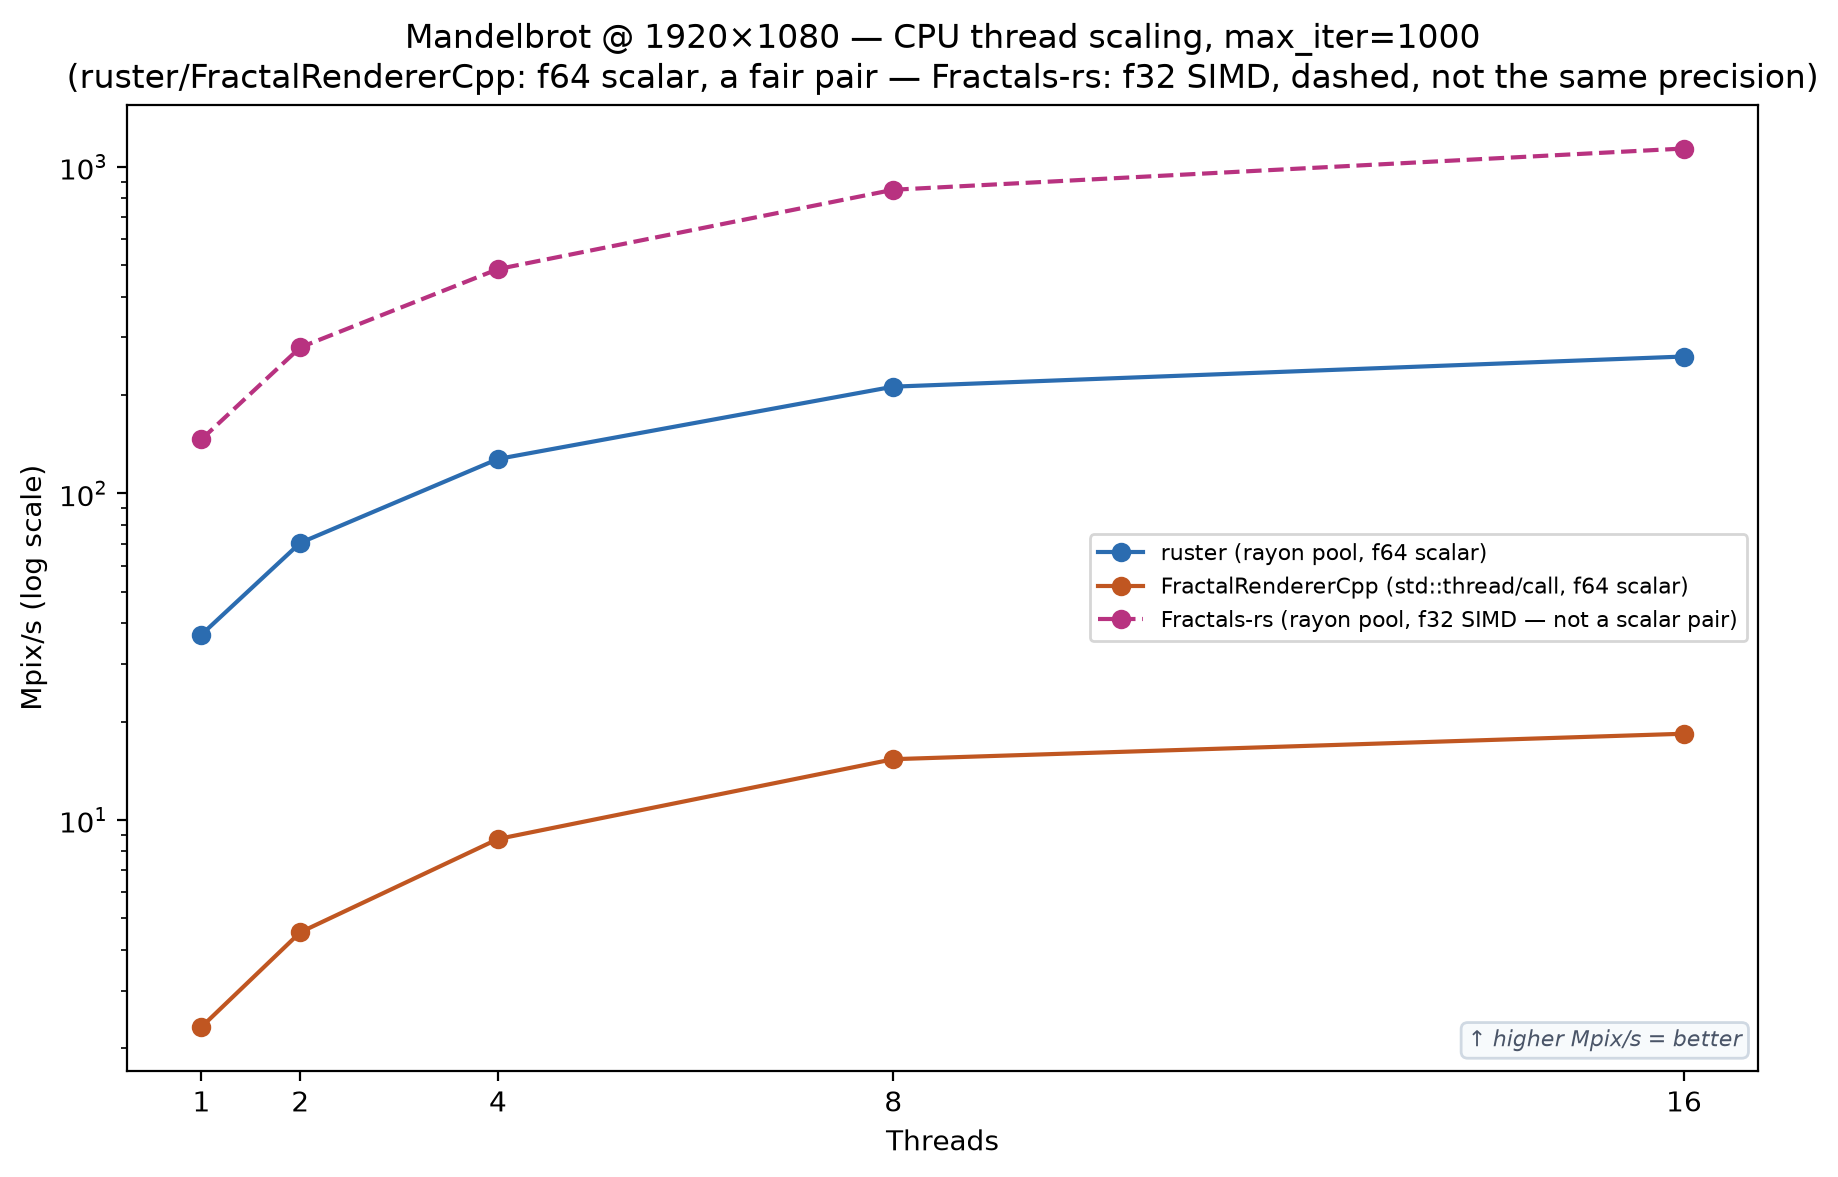
\includegraphics[width=0.7\textwidth]{figures/ruster-thread-scaling.png}
  \caption{CPU thread scaling, ruster vs FractalRendererCpp, Mandelbrot
  1080p, \kod{f64} scalar on both sides.}
  \label{fig:results-thread-scaling}
\end{figure}

Figure~\ref{fig:results-simd-progression} shows the SIMD kernel
progression from Section~\ref{sec:simd}, measured at 1080p and 4K. Each
step, \kod{f64x4}, \kod{f32x8}, then the two chain \kod{f32x8+ILP} kernel,
moves the frame time down, and the pattern repeats almost identically at
both resolutions, evidence that the gain is a property of the kernel
rather than of one particular frame size. The speedup from scalar to
\kod{f32x8+ILP} is $1.92\times$ at 1080p and $2.37\times$ at 4K, with the
instruction level parallelism step contributing under a tenth of that.
Section~\ref{sec:simd} attributes the small residual to the cardioid and
bulb tests already pruning most of the pixels that would otherwise fill
the second chain's pipeline.

\begin{figure}[H]
  \centering
  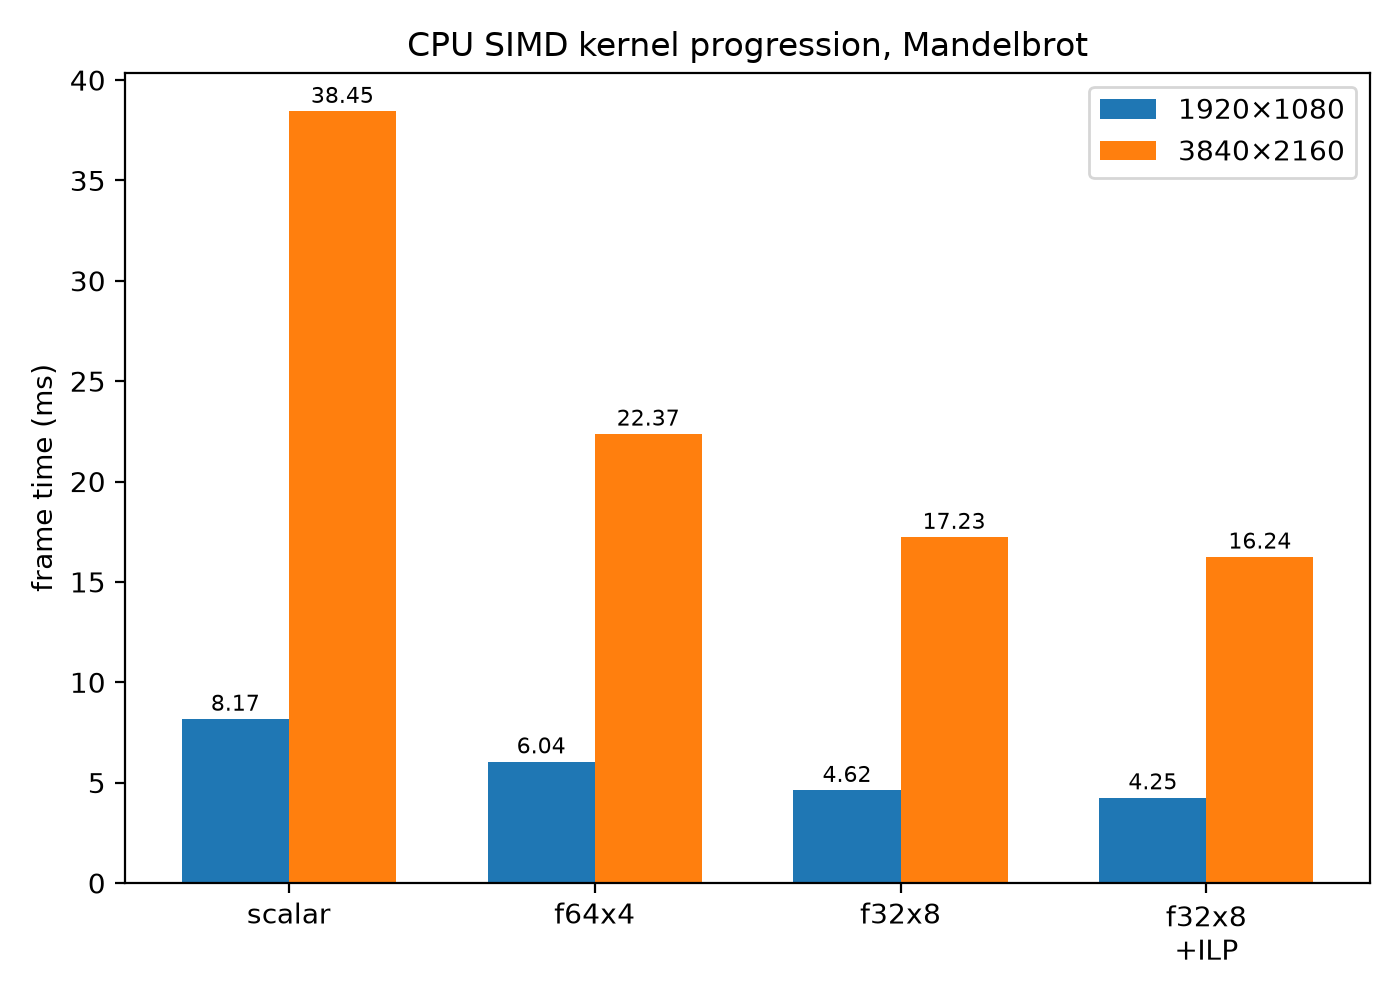
\includegraphics[width=0.75\textwidth]{figures/results-simd-progression.png}
  \caption{CPU SIMD kernel progression, Mandelbrot, 1080p and 4K.}
  \label{fig:results-simd-progression}
\end{figure}

Figure~\ref{fig:results-cpu-microopt} checks two more CPU side choices
against the plain rayon row chunked baseline. The left panel is the
traversal order question from Section~\ref{sec:traversal-locality},
Hilbert tiled traversal against plain row major, and the measured gap
matches that section's claim directly. Hilbert renders slower at every
resolution tested, roughly $224$ against $133$ Mpix/s at $800\times600$
and the gap narrowing but not closing by $3840\times2160$, with no
compensating cache locality win to show for the extra per pixel bit
interleaving cost. The right panel is the instruction level parallelism
question from Section~\ref{sec:simd} on its own, the interleaved
\kod{f32x8+ILP} kernel against plain \kod{f32x8}, and the interleaved
kernel leads at every resolution tested, from a narrow $3\%$ margin at
$800\times600$ to roughly $9\%$ at $1080$p, consistent with a benefit
that needs enough independent per pixel work in flight to be worth the
second chain's bookkeeping.

\begin{figure}[H]
  \centering
  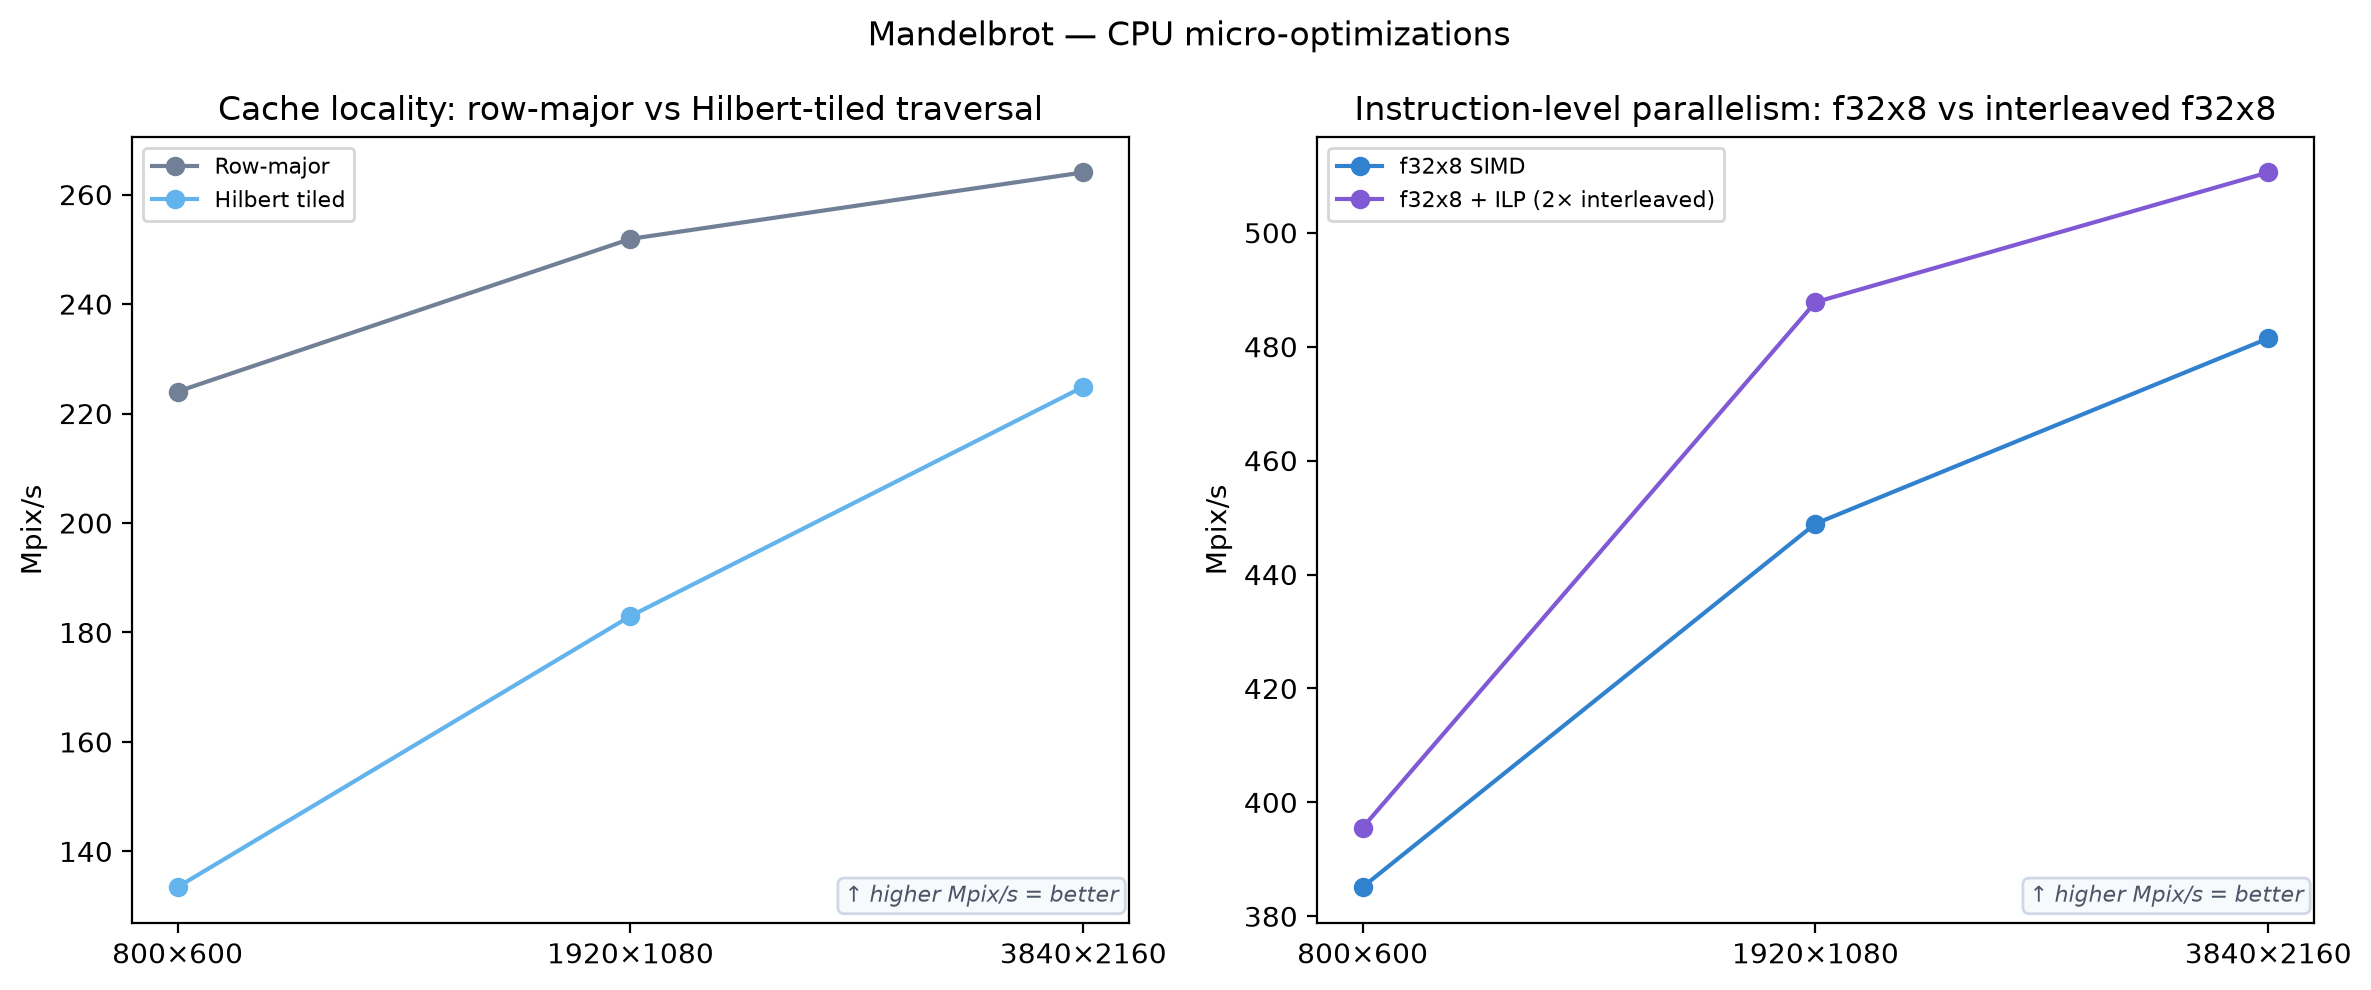
\includegraphics[width=\textwidth]{figures/ruster-cpu-microopt.png}
  \caption{CPU micro optimizations, Hilbert vs row major traversal and
  plain vs interleaved \kod{f32x8}, Mandelbrot.}
  \label{fig:results-cpu-microopt}
\end{figure}

\FloatBarrier

\section{GPU Backends}
\label{sec:results-gpu}

This section's first figure is the chapter's centerpiece. Every
optimization measured exists to move
one number, how many pixels a backend renders per second.
Figure~\ref{fig:results-gpu-resolution} puts every backend this thesis
built on the same axes, CPU scalar, CPU SIMD, CUDA, wgpu, and all four
competitor projects from Section~\ref{sec:bench-cross-renderer}, Fractals-rs,
FractalRendererCpp, XaoS, and FractalNow, at three resolutions, so the
whole CPU to GPU progression is visible in one place rather than
scattered across a chapter's worth of separate panels. XaoS and
FractalNow are measured on their raw per pixel kernel with boundary
tracing and quad interpolation forced off, as
Section~\ref{sec:bench-cross-renderer} explains, not on a measurement of
either project's real interactive engine. A second, hatched XaoS bar
turns boundary tracing back on: $50.8$, $85.3$, and $114.4$ Mpix/s across
the three resolutions, $21\times$ to $36\times$ its own raw kernel and
already ahead of its own multithreaded raw-kernel bar despite running on
a single thread, since \kod{btrace.cpp}'s threaded path is disabled
upstream. It is a single static frame with no previous frame to guess
from, so it measures the boundary-trace-and-flood-fill algorithm alone,
not the additional frame-to-frame reuse XaoS's real zoom animator adds on
top, and is not comparable to any other, multithreaded bar in this
figure.

CUDA leads every other backend at every resolution, wgpu comes second, and
the gap between the two GPU backends stays roughly proportional to frame
size, consistent with a fixed per pixel kernel cost rather than a fixed
per-frame overhead dominating either one. Peak throughput, at
$3840\times2160$, reaches roughly $1389$ Mpix/s on CUDA. The two red
hybrid scheduler bars exist only at $1080$p, since that benchmark group
sweeps zoom at one fixed resolution rather than resolution at one fixed
zoom, and Section~\ref{sec:results-scheduler} reads them directly rather
than through this figure.

\begin{figure}[H]
  \centering
  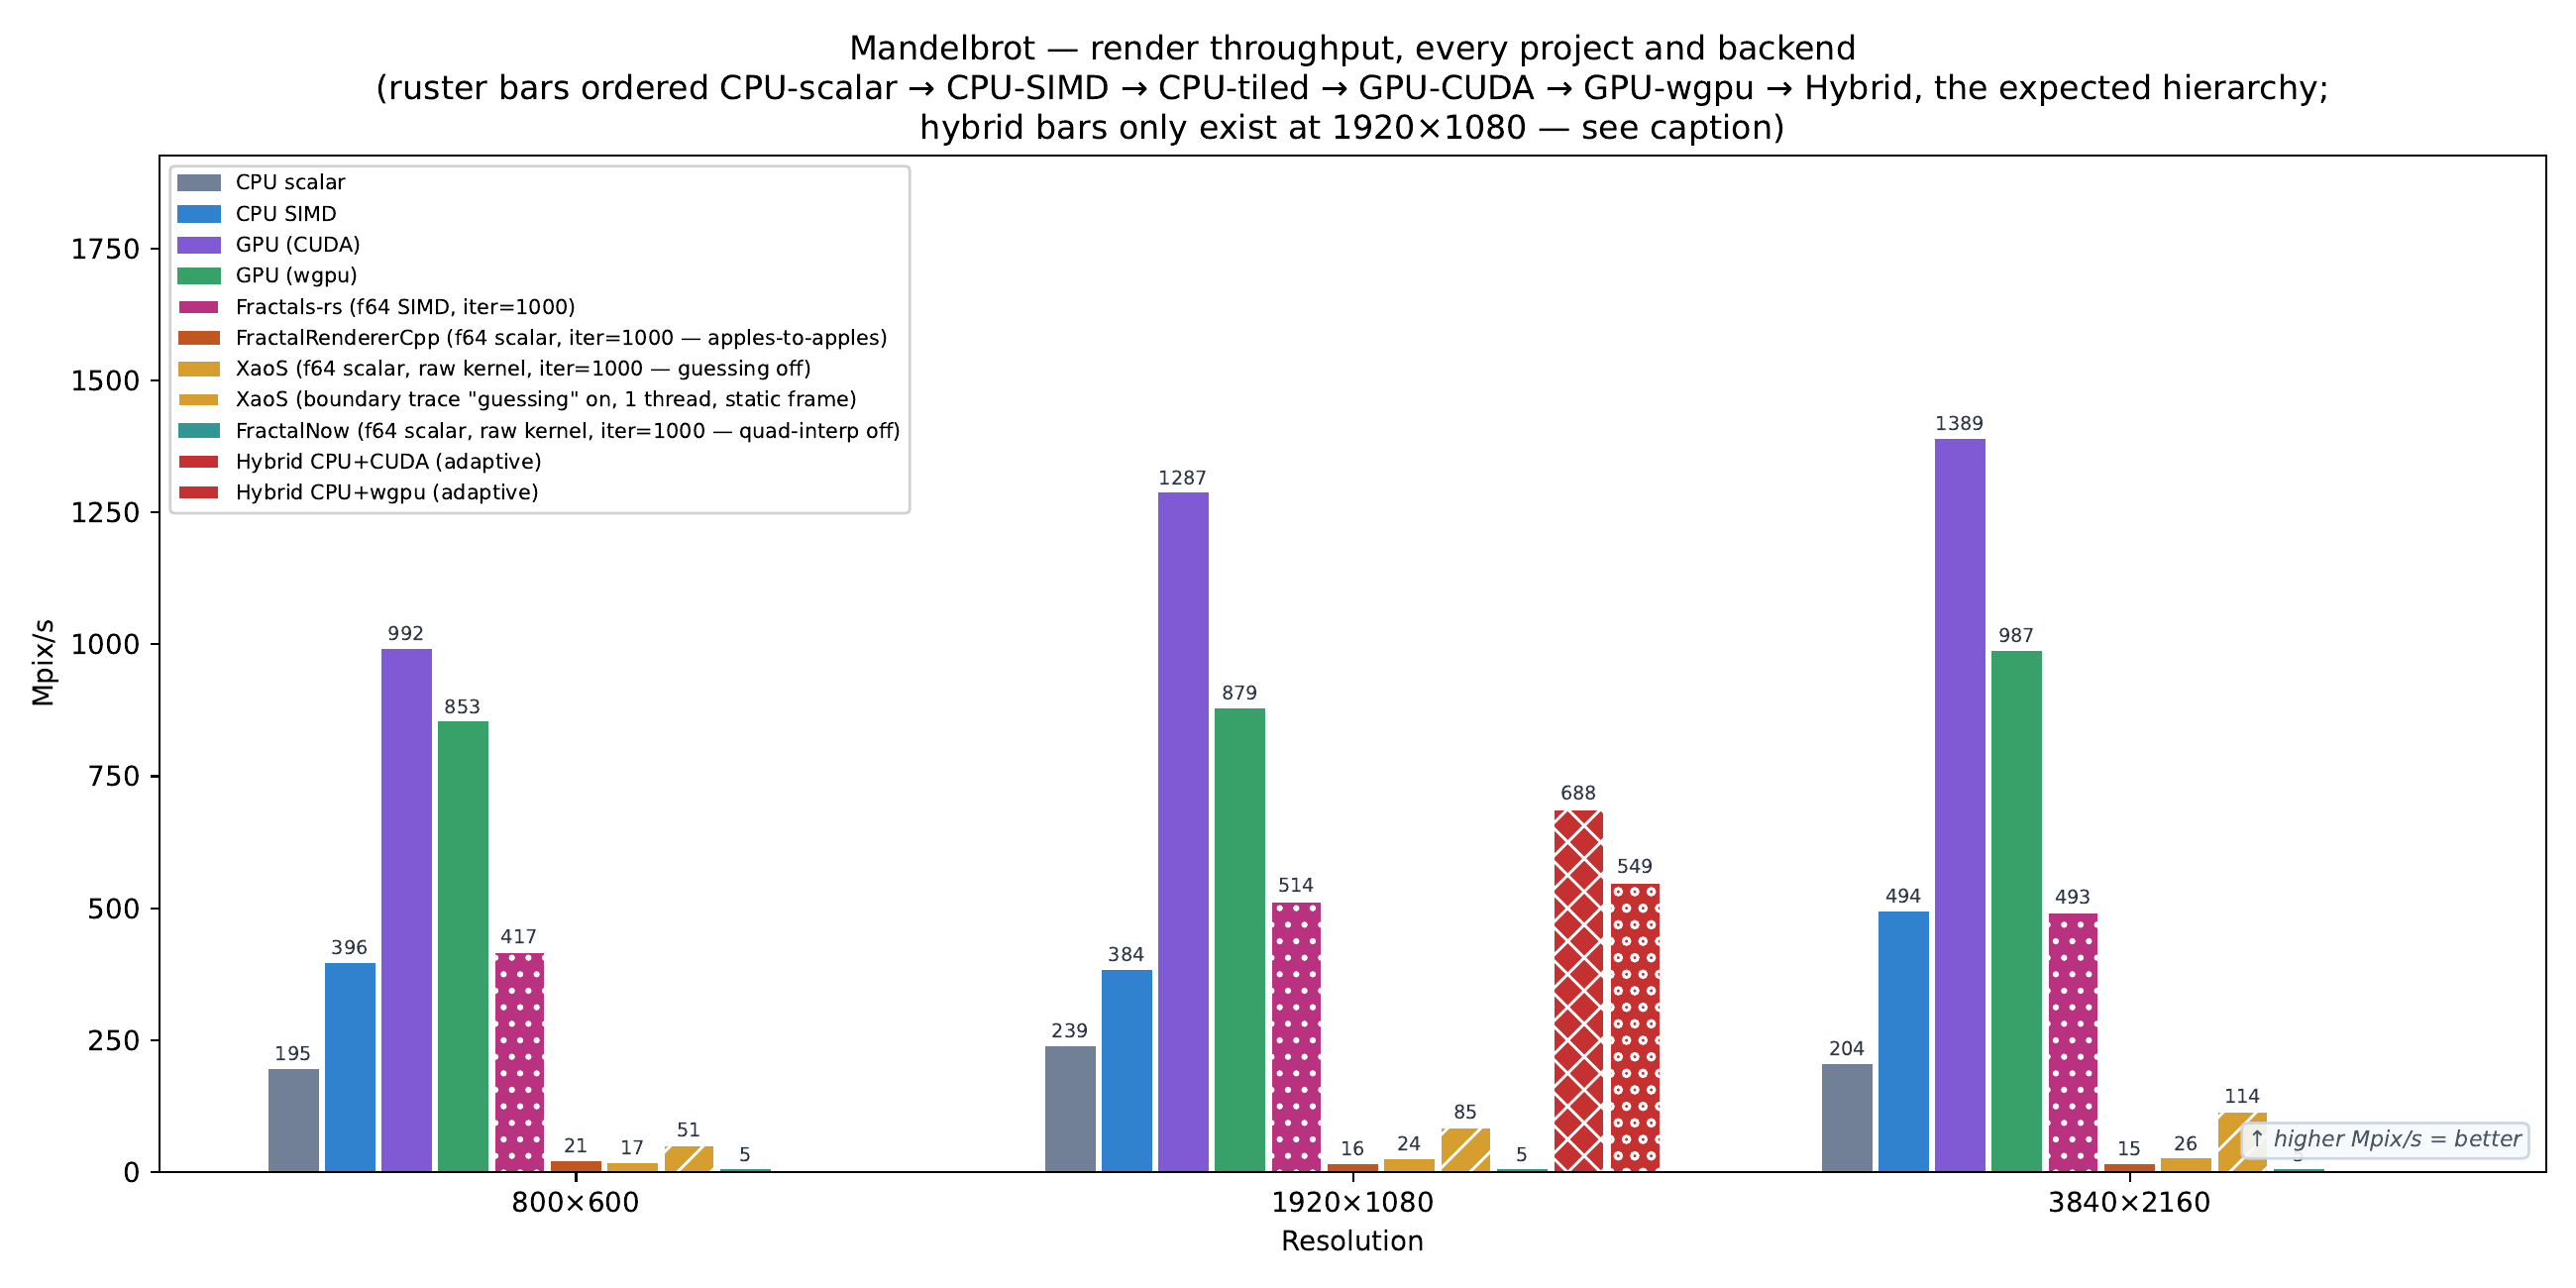
\includegraphics[width=\textwidth]{figures/ruster-throughput-all-backends.png}
  \caption{Render throughput, every ruster backend and all four competitor
  projects, Fractals-rs, FractalRendererCpp, XaoS, FractalNow, three
  resolutions, Mandelbrot, zoom 1. The headline measurement of this
  chapter. Every CPU and GPU optimization from Chapter~\ref{ch:algorithms}
  through Chapter~\ref{ch:gpu} shows up here as the distance between one
  bar and the next. The hatched XaoS bar is its real boundary-trace
  "guessing" algorithm, single thread, single static frame, not
  comparable to the multithreaded bars around it.}
  \label{fig:results-gpu-resolution}
\end{figure}

Read left to right within any one resolution group, the bars trace the
whole optimization path this thesis takes. Scalar to SIMD is
Chapter~\ref{ch:algorithms}'s work, SIMD to either GPU backend is
Chapter~\ref{ch:gpu}'s. CUDA's lead over CPU SIMD, roughly $2.5\times$ to
$3.4\times$ depending on resolution, is the return on building a GPU
backend at all, and the rest of this section explains where inside that
CUDA number the time actually goes.

Figure~\ref{fig:results-gpu-breakdown} isolates why CUDA wins the frame.
The two kernels are within $5\%$ of each other, but host readback is
$83\%$ of the CUDA frame and $88\%$ of the wgpu frame, and wgpu pays
roughly $0.8\,\mathrm{ms}$ more of it, consistent with the extra device
to device staging copy that CUDA's single \kod{dtoh\_sync\_copy} avoids,
as Section~\ref{sec:cuda} explains.

\begin{figure}[H]
  \centering
  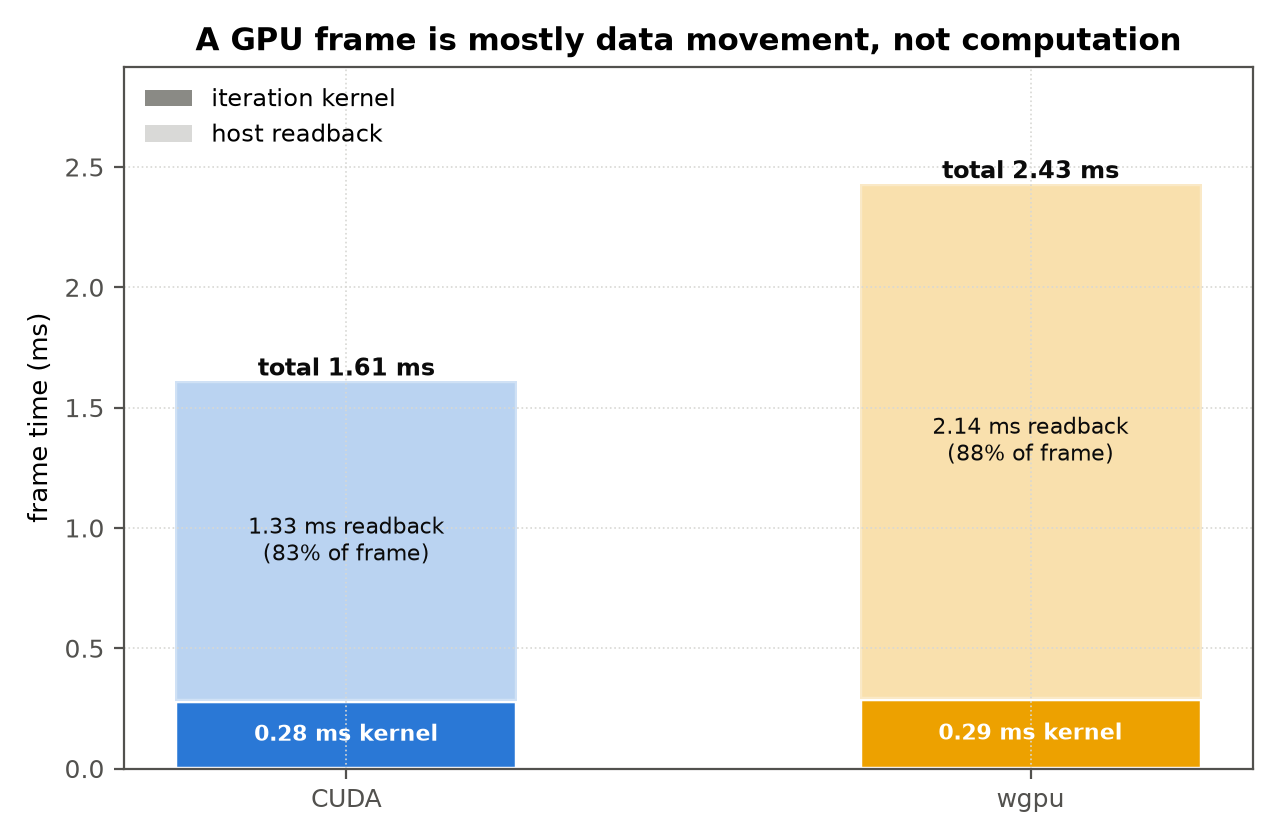
\includegraphics[width=0.7\textwidth]{figures/results-gpu-frame-breakdown.png}
  \caption{GPU frame time breakdown, kernel vs host readback, CUDA vs
  wgpu, $1920\times1080$, zoom 1.}
  \label{fig:results-gpu-breakdown}
\end{figure}

Both GPU backends, in other words, spend most of a frame moving pixels
back to the host, not computing them. That reframes
Section~\ref{sec:results-pipeline}'s question before it is even asked.
If a GPU backend is already dominated by data movement rather than
iteration, adding a CPU side \kod{colorize()} stage on top can only make
that imbalance more visible, not less, unless that stage moves to the
GPU too, which, for CUDA, it has, as Section~\ref{sec:gpu-traversal}
describes.

\FloatBarrier

\section{End to End Pipeline}
\label{sec:results-pipeline}

Figure~\ref{fig:results-pipeline} adds the \kod{colorize()} step as
measured before either GPU backend could skip it, run on the CPU for
every backend alike. The GPU's advantage over the CPU narrows sharply
once that fixed $2.72\,\mathrm{ms}$ stage is included, from roughly
$5.4\times$ on the render stage alone to $2.09\times$ for CUDA and
$1.72\times$ for wgpu end to end. Of a $5.19\,\mathrm{ms}$ CUDA pipeline,
roughly $0.4\,\mathrm{ms}$ is fractal iteration, and the remaining
$4.8\,\mathrm{ms}$ is data movement and coloring. That is exactly what
made moving \kod{colorize()} onto the GPU the single highest leverage
optimization this measurement pointed at, larger than the fp64 bulb fix
in Section~\ref{sec:cuda} and larger than anything the scheduler in
Chapter~\ref{ch:scheduler} can recover. CUDA's \kod{colorize()} has since
moved on device through \kod{colorize\_kernel} and
\kod{render\_and\_colorize}, described in Section~\ref{sec:gpu-traversal},
pixel exact against the CPU version and $54\%$ to $63\%$ faster end to
end at the shallow and mid zooms where colorize used to dominate frame
time. wgpu and the heterogeneous scheduler still colorize on the CPU.
The scheduler does so by necessity, since its merged buffer only ever
exists on the host side, as Chapter~\ref{ch:scheduler} explains, so the
gain above remains open for those two paths.

\begin{figure}[H]
  \centering
  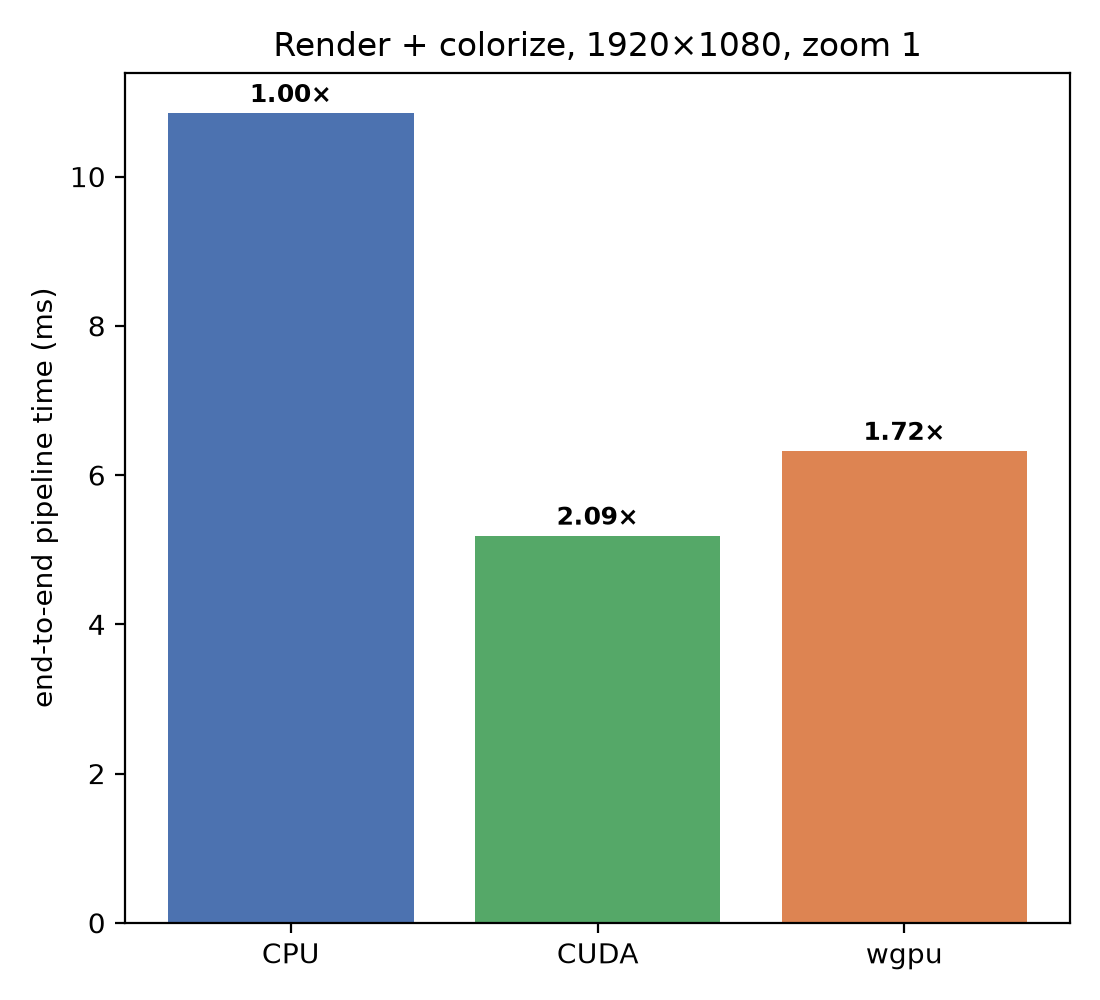
\includegraphics[width=0.65\textwidth]{figures/results-pipeline-end-to-end.png}
  \caption{End to end pipeline time, render plus colorize, $1920\times1080$,
  zoom 1. Measured with colorize run on the CPU for every backend, before
  CUDA's own colorize step moved on device, see prose.}
  \label{fig:results-pipeline}
\end{figure}

Figure~\ref{fig:results-colorize-overhead} breaks the same stage down per
backend, render only against render plus colorize, from that same
measurement where every backend colorized on the CPU. The fixed
\kod{colorize()} cost took a bigger proportional bite out of a GPU
backend than out of the CPU, since it was the same CPU side stage every
time, roughly a fifth off the CPU's own throughput but closer to two
thirds off either GPU backend's, the same Amdahl effect
Figure~\ref{fig:results-pipeline} already shows stated as an absolute
time rather than a proportion. This is precisely the effect that made
moving colorize onto the GPU worth doing for CUDA.

\begin{figure}[H]
  \centering
  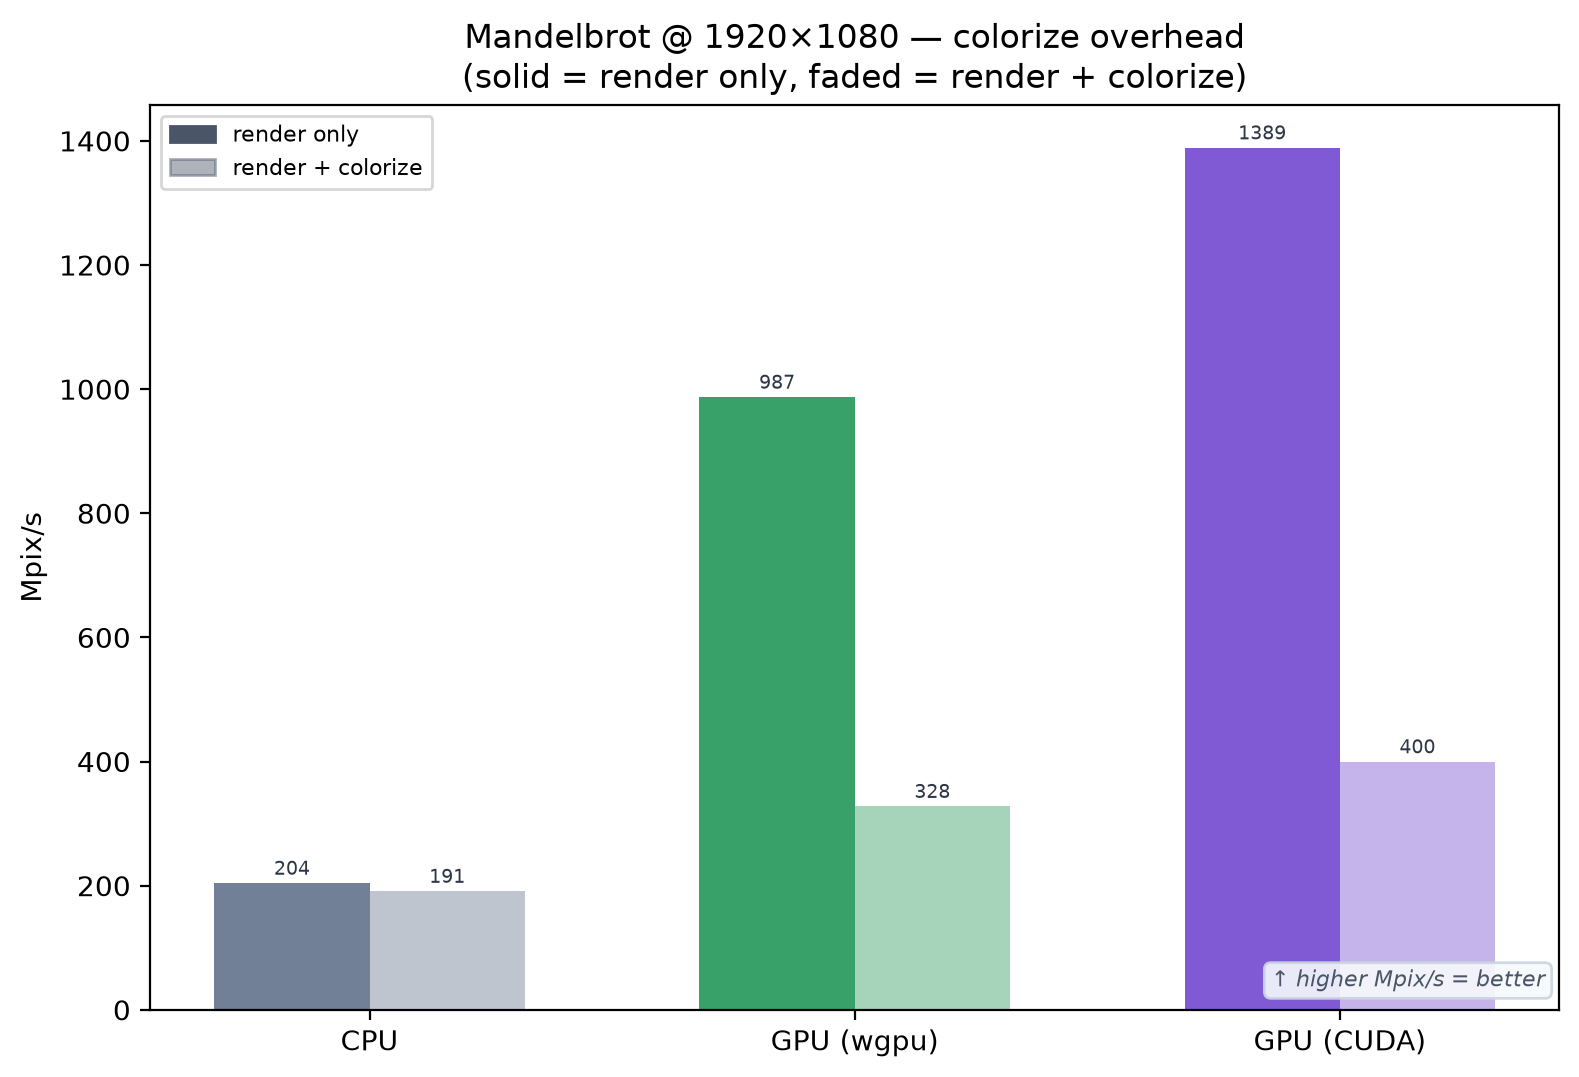
\includegraphics[width=0.6\textwidth]{figures/ruster-colorize-overhead.png}
  \caption{Colorize overhead per backend, render only vs render plus
  colorize, Mandelbrot.}
  \label{fig:results-colorize-overhead}
\end{figure}

Chapter~\ref{ch:scheduler}'s scheduler exists to buy back exactly the time
this section just spent two figures accounting for, so that is where this
chapter turns to next.

\FloatBarrier

\section{Hybrid CPU+GPU Scheduler}
\label{sec:results-scheduler}

This section is where the thesis's central claim gets tested against
data. Chapter~\ref{ch:scheduler} built a scheduler that watches both
devices at runtime and routes tiles by measured cost instead of dividing
a frame blindly. The two figures here are the evidence for whether that
machinery earns its keep, at a shallow zoom where it should struggle and
at a deep zoom sweep where it is designed to win.

Figure~\ref{fig:results-sched-shallow} measures the scheduler from
Chapter~\ref{ch:scheduler} against both solo backends and the naive
static split, at zoom 1. The static $50/50$ CPU plus wgpu split, with no
classification at all, is the worst active configuration on the chart,
$408$ against wgpu's own $879$ Mpix/s solo. That is exactly the failure
Section~\ref{sec:work-distribution} motivates the corner sampling
classifier by, an even split leaves the faster device waiting on the
slower one. The adaptive scheduler recovers most of that loss, $688$
Mpix/s on CUDA and $549$ on wgpu, but still trails using either GPU alone.
Every scheduler configuration loses to simply using the better GPU alone
at this zoom, the Section~\ref{sec:scheduler-motivation} arithmetic
showing through directly, its own machinery costs a fixed amount, and the
kernel time it can shrink is a small fraction of an already GPU dominated
frame. At shallow zoom, in short, there is not enough imbalance between
devices for a scheduler to fix.

\begin{figure}[H]
  \centering
  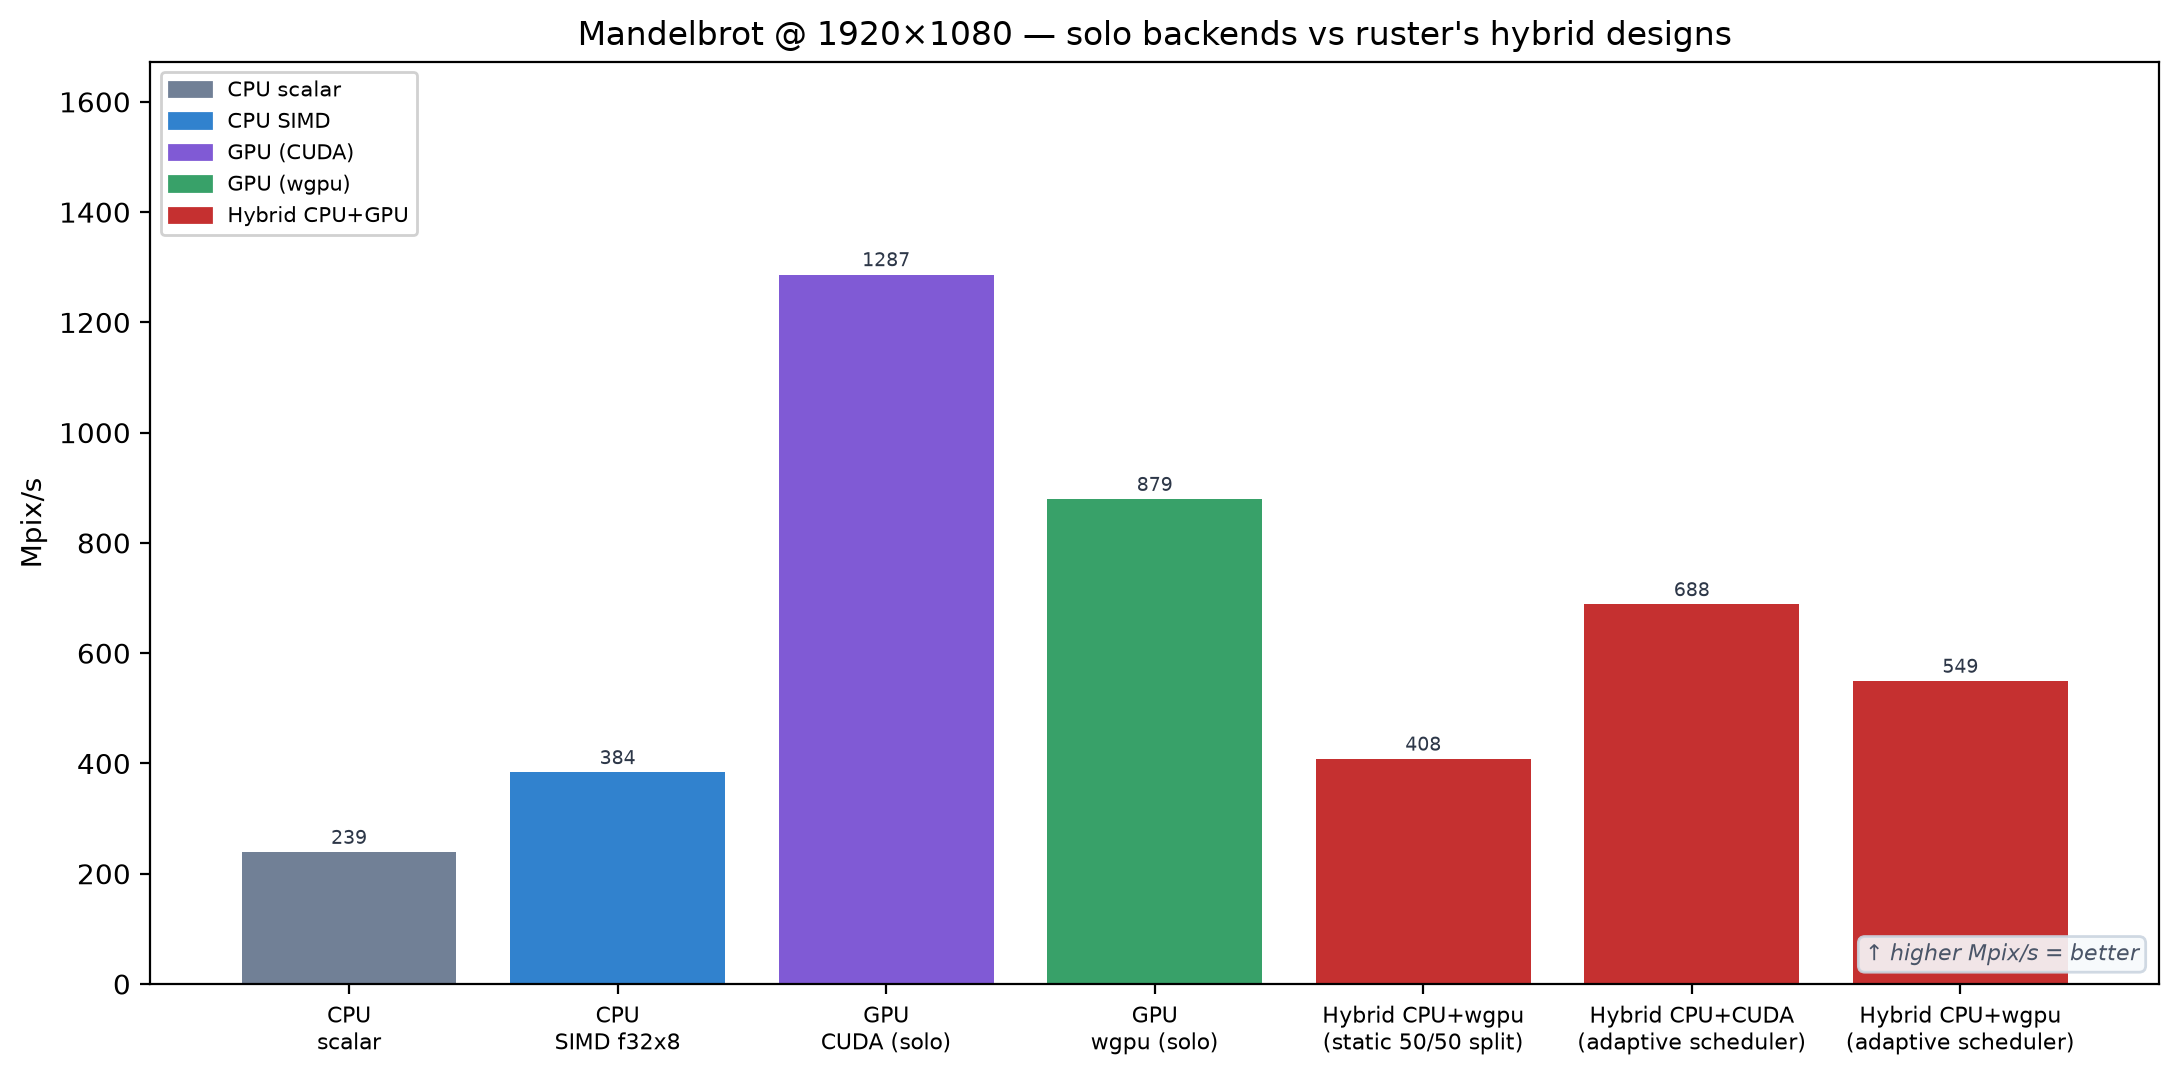
\includegraphics[width=0.75\textwidth]{figures/ruster-solo-vs-hybrid.png}
  \caption{Solo backends vs the static split and the adaptive scheduler,
  Mandelbrot 1080p, zoom 1.}
  \label{fig:results-sched-shallow}
\end{figure}

Deep zoom is a different regime, and it is where this thesis's central
result actually lives. Figure~\ref{fig:results-sched-deepzoom} extends the
same comparison from zoom $10^4$ to $10^{15}$. Right at the $10^6$
precision threshold Section~\ref{sec:bench-zoom-sweeps} sweeps around,
CUDA's own fallback from \kod{f32} to \kod{f64} lands it briefly above the
CPU, $218$ against $130\,\mathrm{ms}$, before both devices settle within
about $1.1\times$ of each other from $10^7$ onward. That crossing is
exactly where the scheduler pays off. At zoom $10^6$ it beats not only
the better solo backend, the CPU at that specific zoom, but the ideal
proportional split too, $74.3$ against $81.6\,\mathrm{ms}$, a
$1.75\times$ win over the better device that is direct evidence for this
thesis's central claim, corner sampling classification routes expensive
tiles to the CPU instead of dividing the frame blindly, and that routing
is worth more than an even split even when an even split is the
theoretically available ceiling. The wins past $10^7$ are smaller,
roughly $1.13\times$ to $1.15\times$, and leave roughly $43\%$ of the
available headroom on the table by the load balancer's own numbers, since
the ideal split reaches roughly $45\,\mathrm{ms}$ at those zooms while the
hybrid scheduler still measures near $79\,\mathrm{ms}$, a tuning problem
in a regime this benchmark suite only now covers, not a structural one.

\begin{figure}[H]
  \centering
  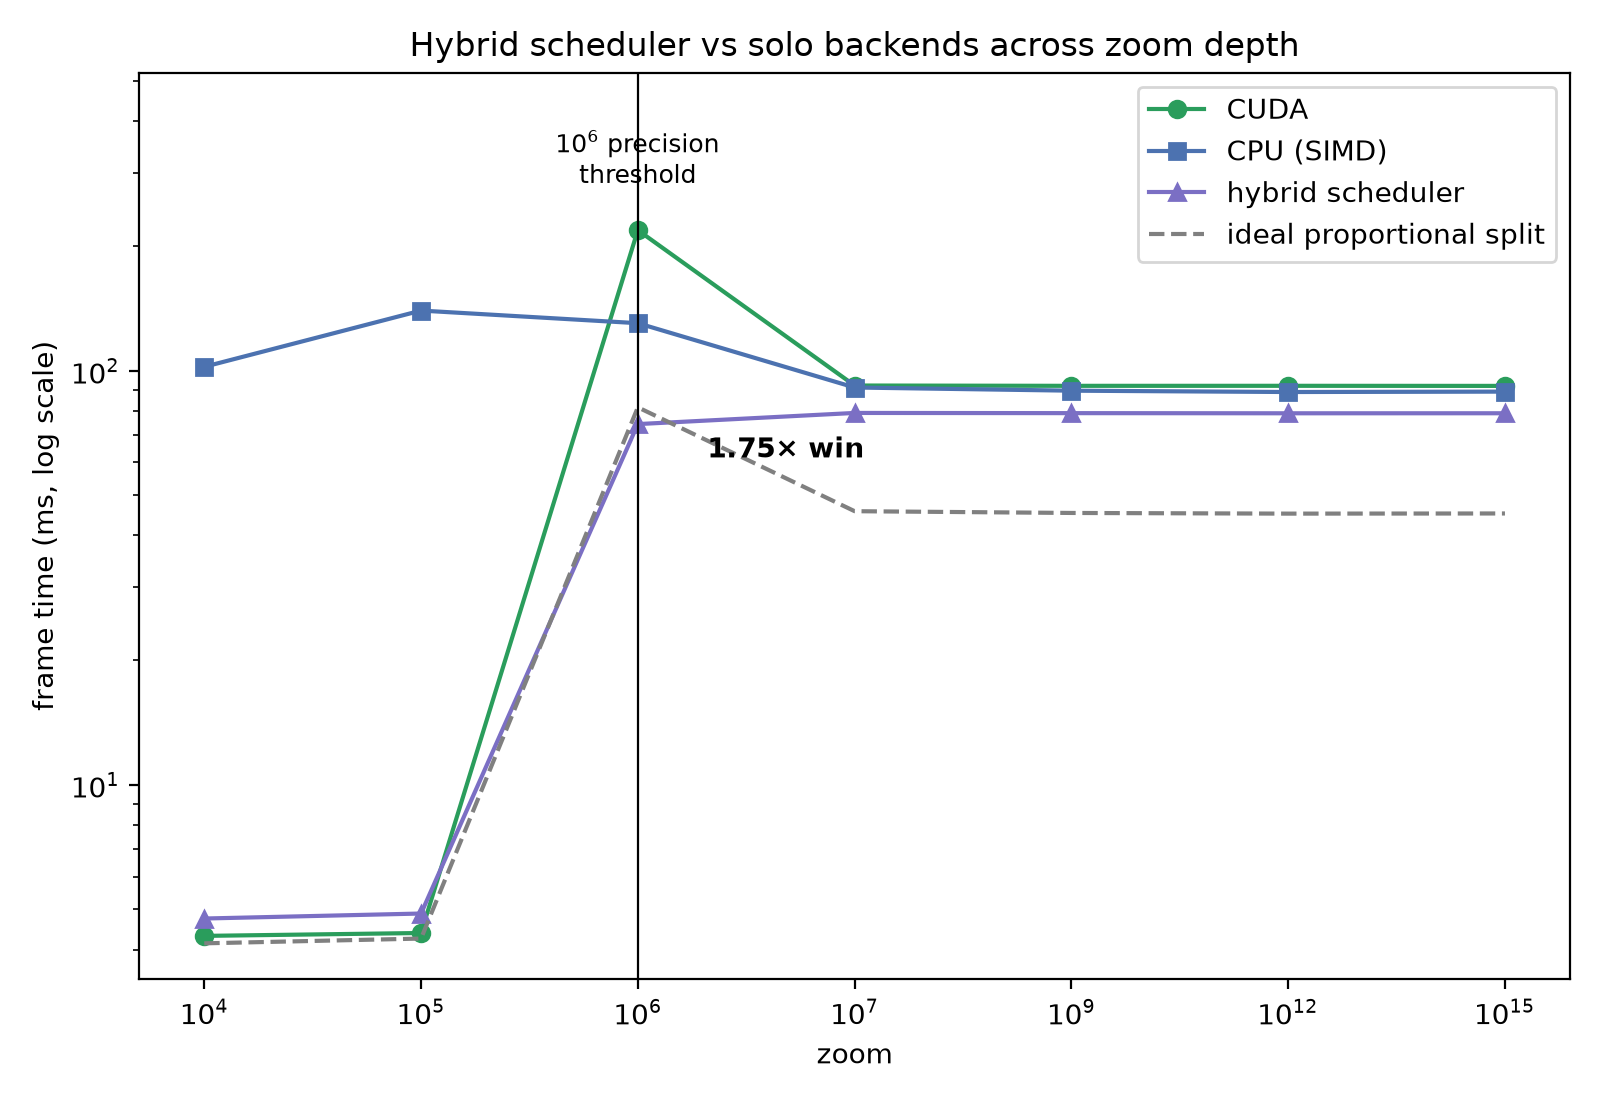
\includegraphics[width=\textwidth]{figures/results-scheduler-deepzoom.png}
  \caption{Hybrid scheduler vs solo backends and the ideal proportional
  split, across zoom depth, Mandelbrot, seahorse valley. The $1.75\times$
  win at $10^6$ is this thesis's clearest evidence that corner sampling
  classification, not just having two devices, is what the hybrid
  scheduler contributes.}
  \label{fig:results-sched-deepzoom}
\end{figure}

The two figures together answer the question Chapter~\ref{ch:scheduler}
opened with. A scheduler is only worth its complexity where devices are
imbalanced enough for routing to matter. It loses at shallow zoom because
there is nothing to route around, and it wins precisely where
Section~\ref{sec:scheduler-motivation} predicted it would, at the
precision cliff where one device suddenly costs far more per tile than
the other.

\FloatBarrier

\section{Perturbation Theory}
\label{sec:results-perturbation}

Figure~\ref{fig:results-perturbation-zoom} measures perturbation theory,
described in Section~\ref{sec:perturbation}, against the plain direct
kernel, per backend, from zoom $1$ to $10^{12}$. Perturbation never wins
in this range, on any of the three backends. The gap is starkest on CUDA,
where the naive kernel's own \kod{f32} fast path renders the shallow end
of the sweep at well over $1000$ Mpix/s while perturbation, restricted to
\kod{f64} throughout as Section~\ref{sec:cuda} explains, stays flat near
the bottom of the chart the whole way across. That confirms
Section~\ref{sec:perturbation}'s own conclusion directly, this sweep
never reaches a zoom where plain \kod{f64} actually breaks down, so
perturbation is pure overhead here rather than the correctness feature it
becomes only at zoom levels beyond what any backend's direct kernel can
represent at all.

\begin{figure}[H]
  \centering
  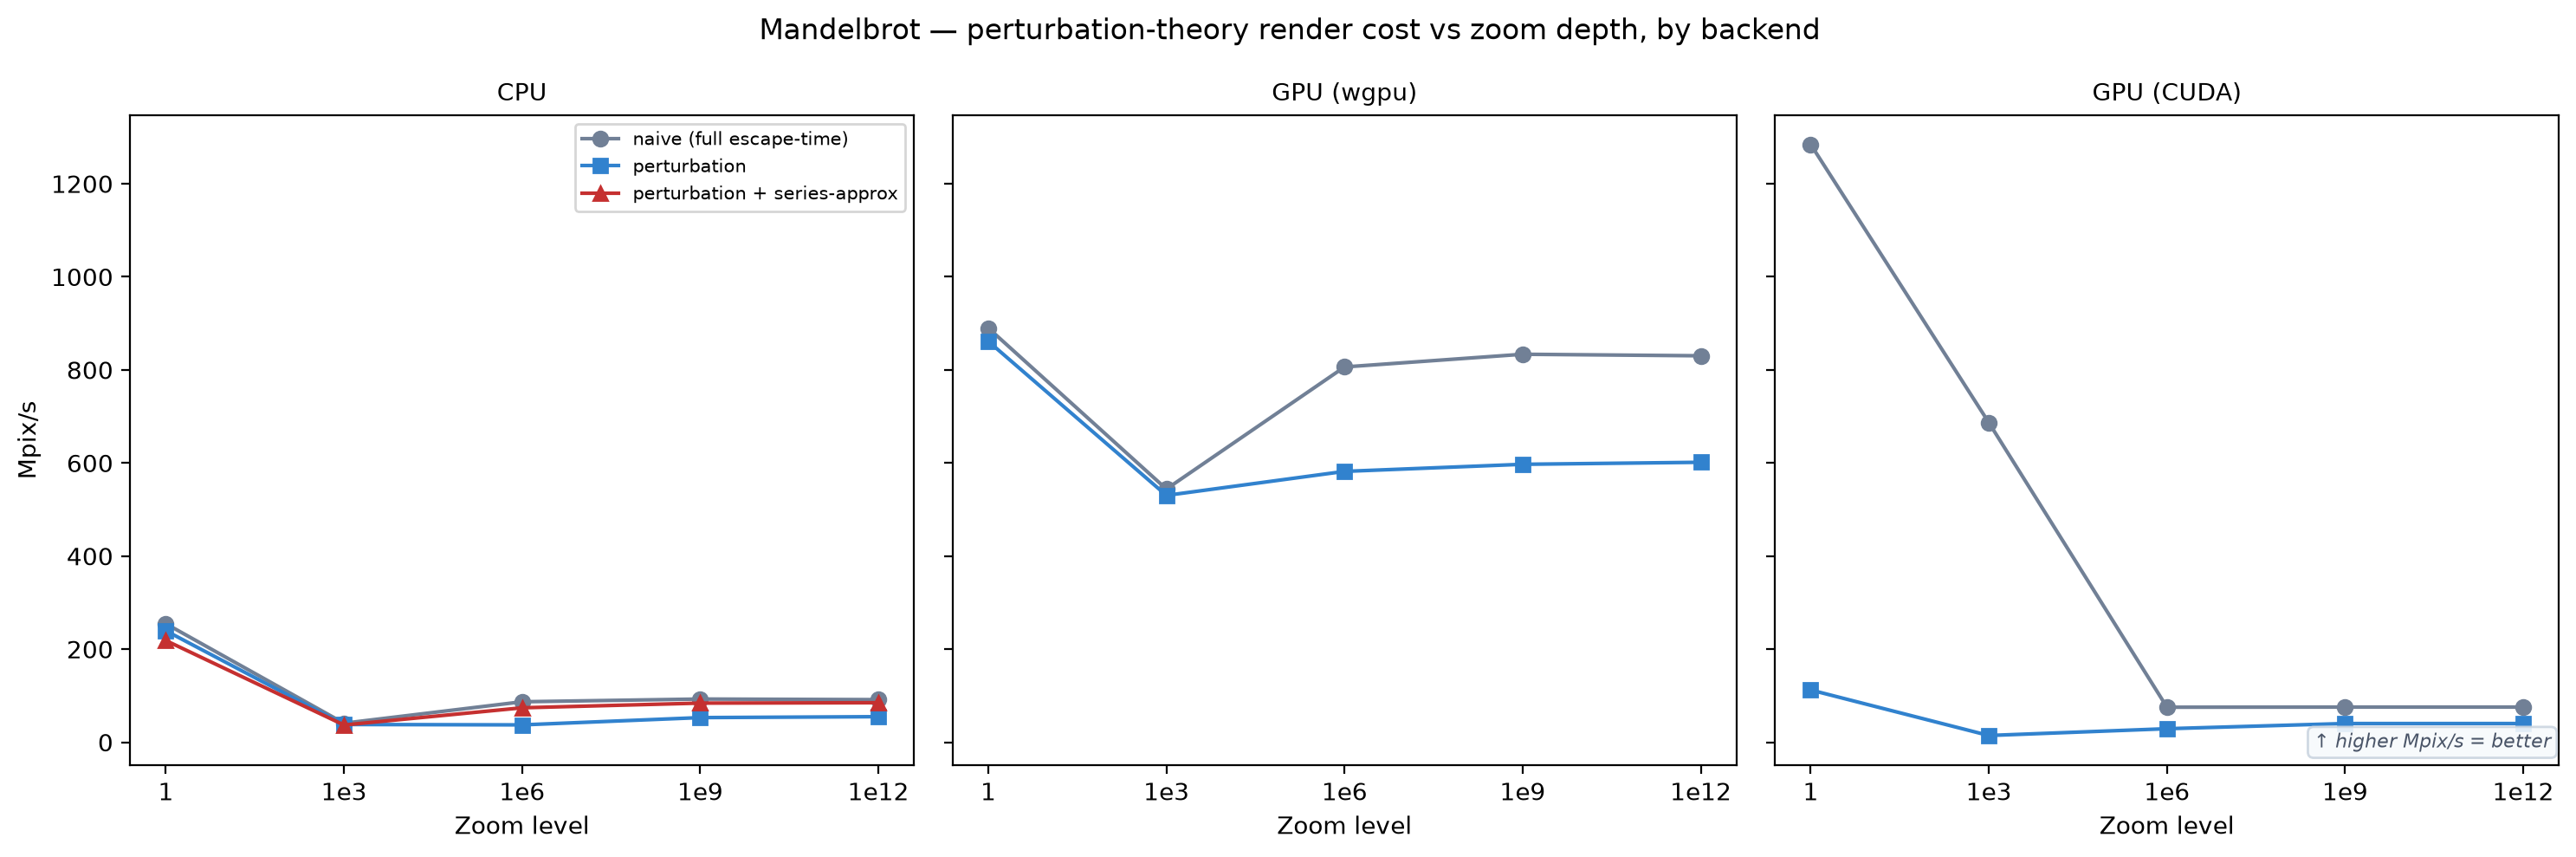
\includegraphics[width=\textwidth]{figures/ruster-perturbation-vs-zoom.png}
  \caption{Perturbation theory vs the plain direct kernel, per backend,
  across zoom depth, Mandelbrot.}
  \label{fig:results-perturbation-zoom}
\end{figure}

Figure~\ref{fig:results-perturbation-internals} explains why that
overhead is cheap enough to be a reasonable trade once it is needed. The
double-double reference orbit from Section~\ref{sec:precision} costs
roughly three times its plain \kod{f64} counterpart per call, $0.0010$
against $0.0003\,\mathrm{ms}$, and the series approximation coefficients
from Section~\ref{sec:series-approximation} grow roughly tenfold from
shallow to deep zoom. Both numbers stay well under a microsecond,
negligible next to a millisecond scale frame, which is exactly why
Section~\ref{sec:precision} can afford to pay the double-double cost once
per frame rather than once per pixel.

\begin{figure}[H]
  \centering
  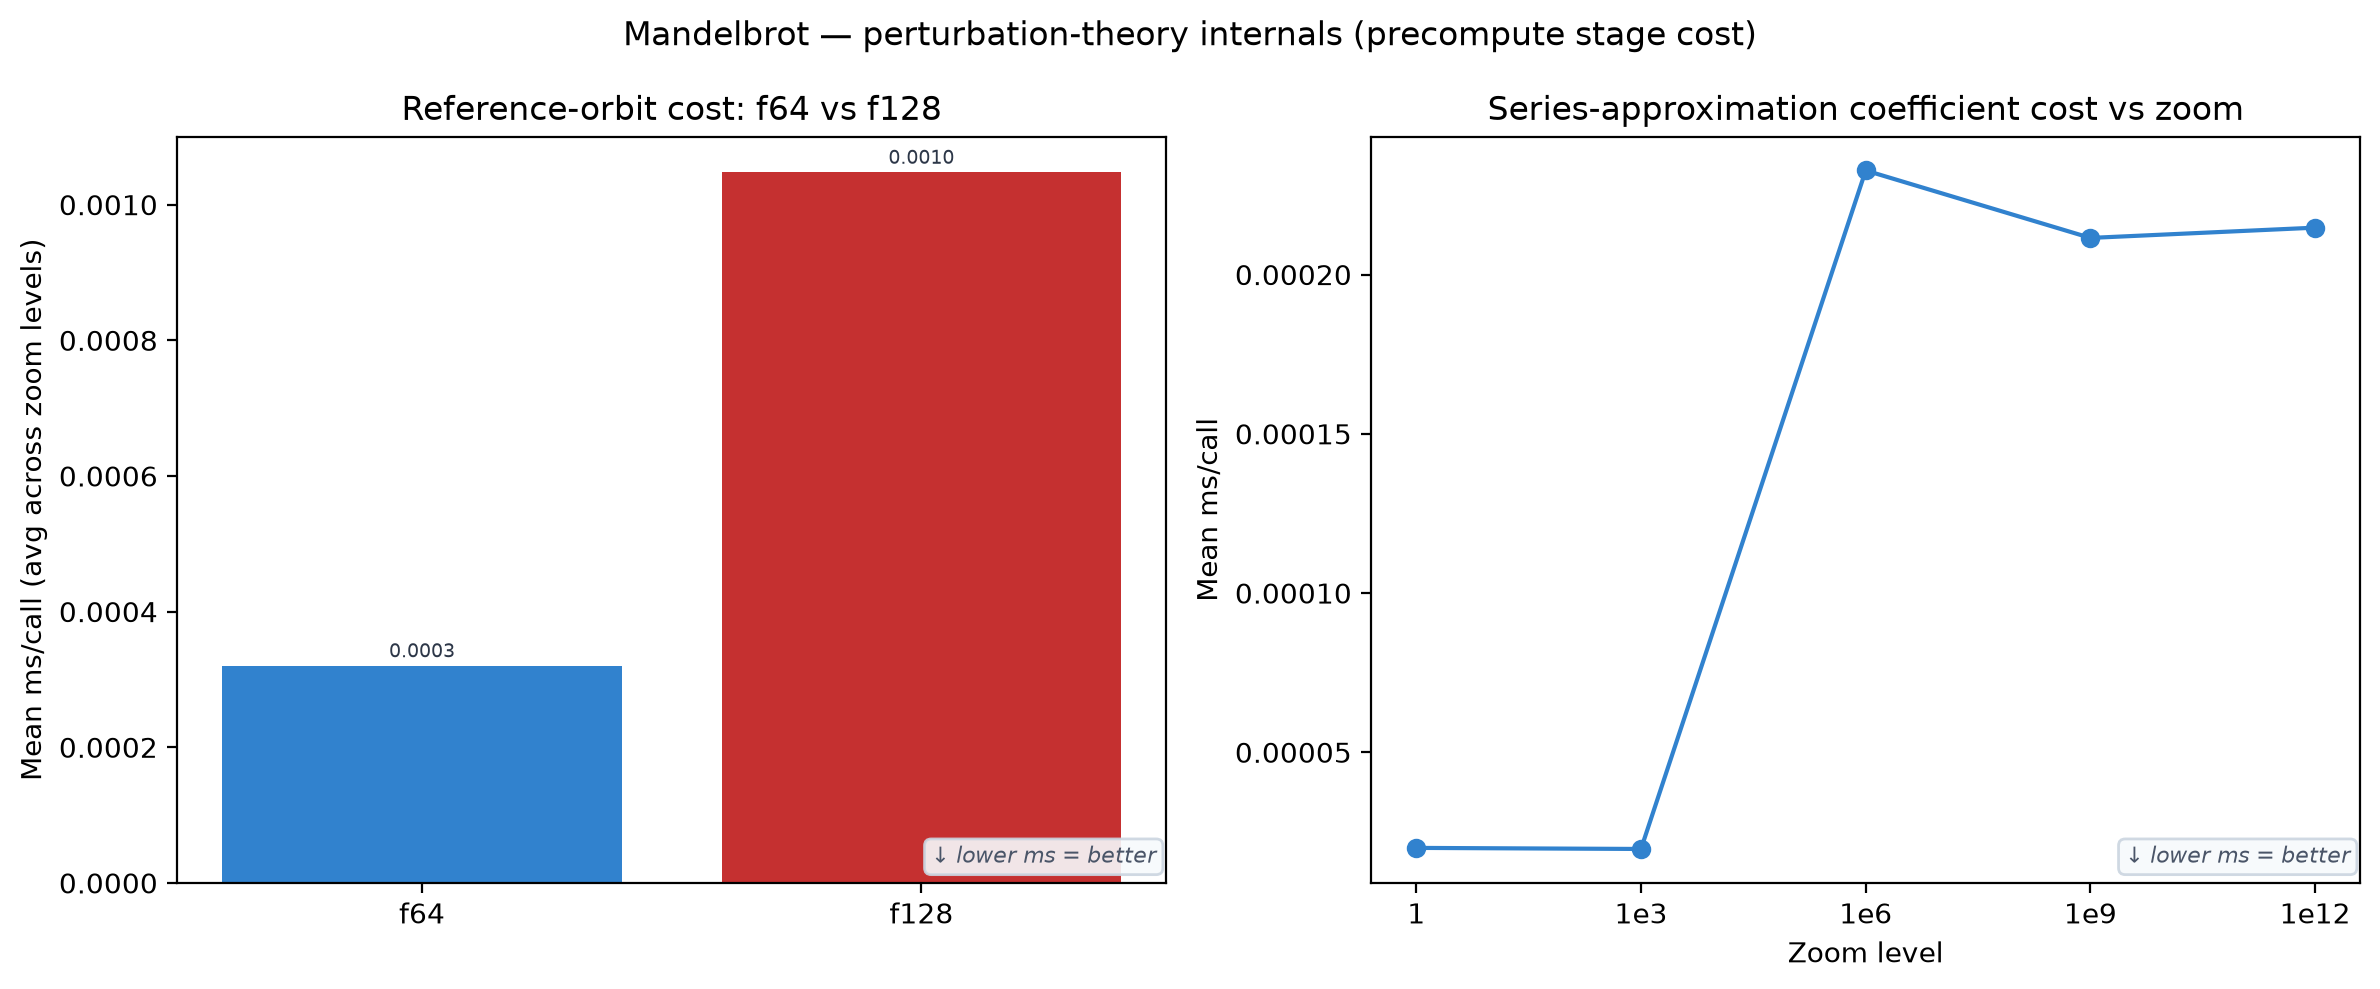
\includegraphics[width=0.85\textwidth]{figures/ruster-perturbation-internals.png}
  \caption{Perturbation precompute cost, \kod{f64} vs \kod{f128} reference
  orbit and series approximation coefficients vs zoom.}
  \label{fig:results-perturbation-internals}
\end{figure}

Perturbation theory costs almost nothing to keep switched on, then, even
in the benchmark range where it never pays for itself. The next section
turns from ruster's own backends to how the whole renderer stacks up
against the four competing projects Section~\ref{sec:related-work}
surveyed.

\FloatBarrier

\section{Cross-Project Comparison}
\label{sec:results-cross-project}

Figure~\ref{fig:results-cross-project} places ruster against the three
competitor renderers across every metric class this thesis measures for
them, single pixel kernel cost, full frame render at three resolutions,
thread scaling from one to sixteen threads, and, where available, the
full pipeline, all under the protocol Section~\ref{sec:bench-cross-renderer}
sets out, matched resolution, iteration count, and view. ruster leads
every panel, by roughly one order of magnitude over the fastest
competitor and two over the slowest, at every thread count and every
resolution tested. The pipeline panel only has data for
FractalRendererCpp and FractalNow, since XaoS's and FractalNow's own
"guessing" shortcuts, described in Section~\ref{sec:bench-cross-renderer},
apply to a full colored frame, not to ruster's split render and colorize
measurement, so the two are not directly comparable there.

\begin{figure}[H]
  \centering
  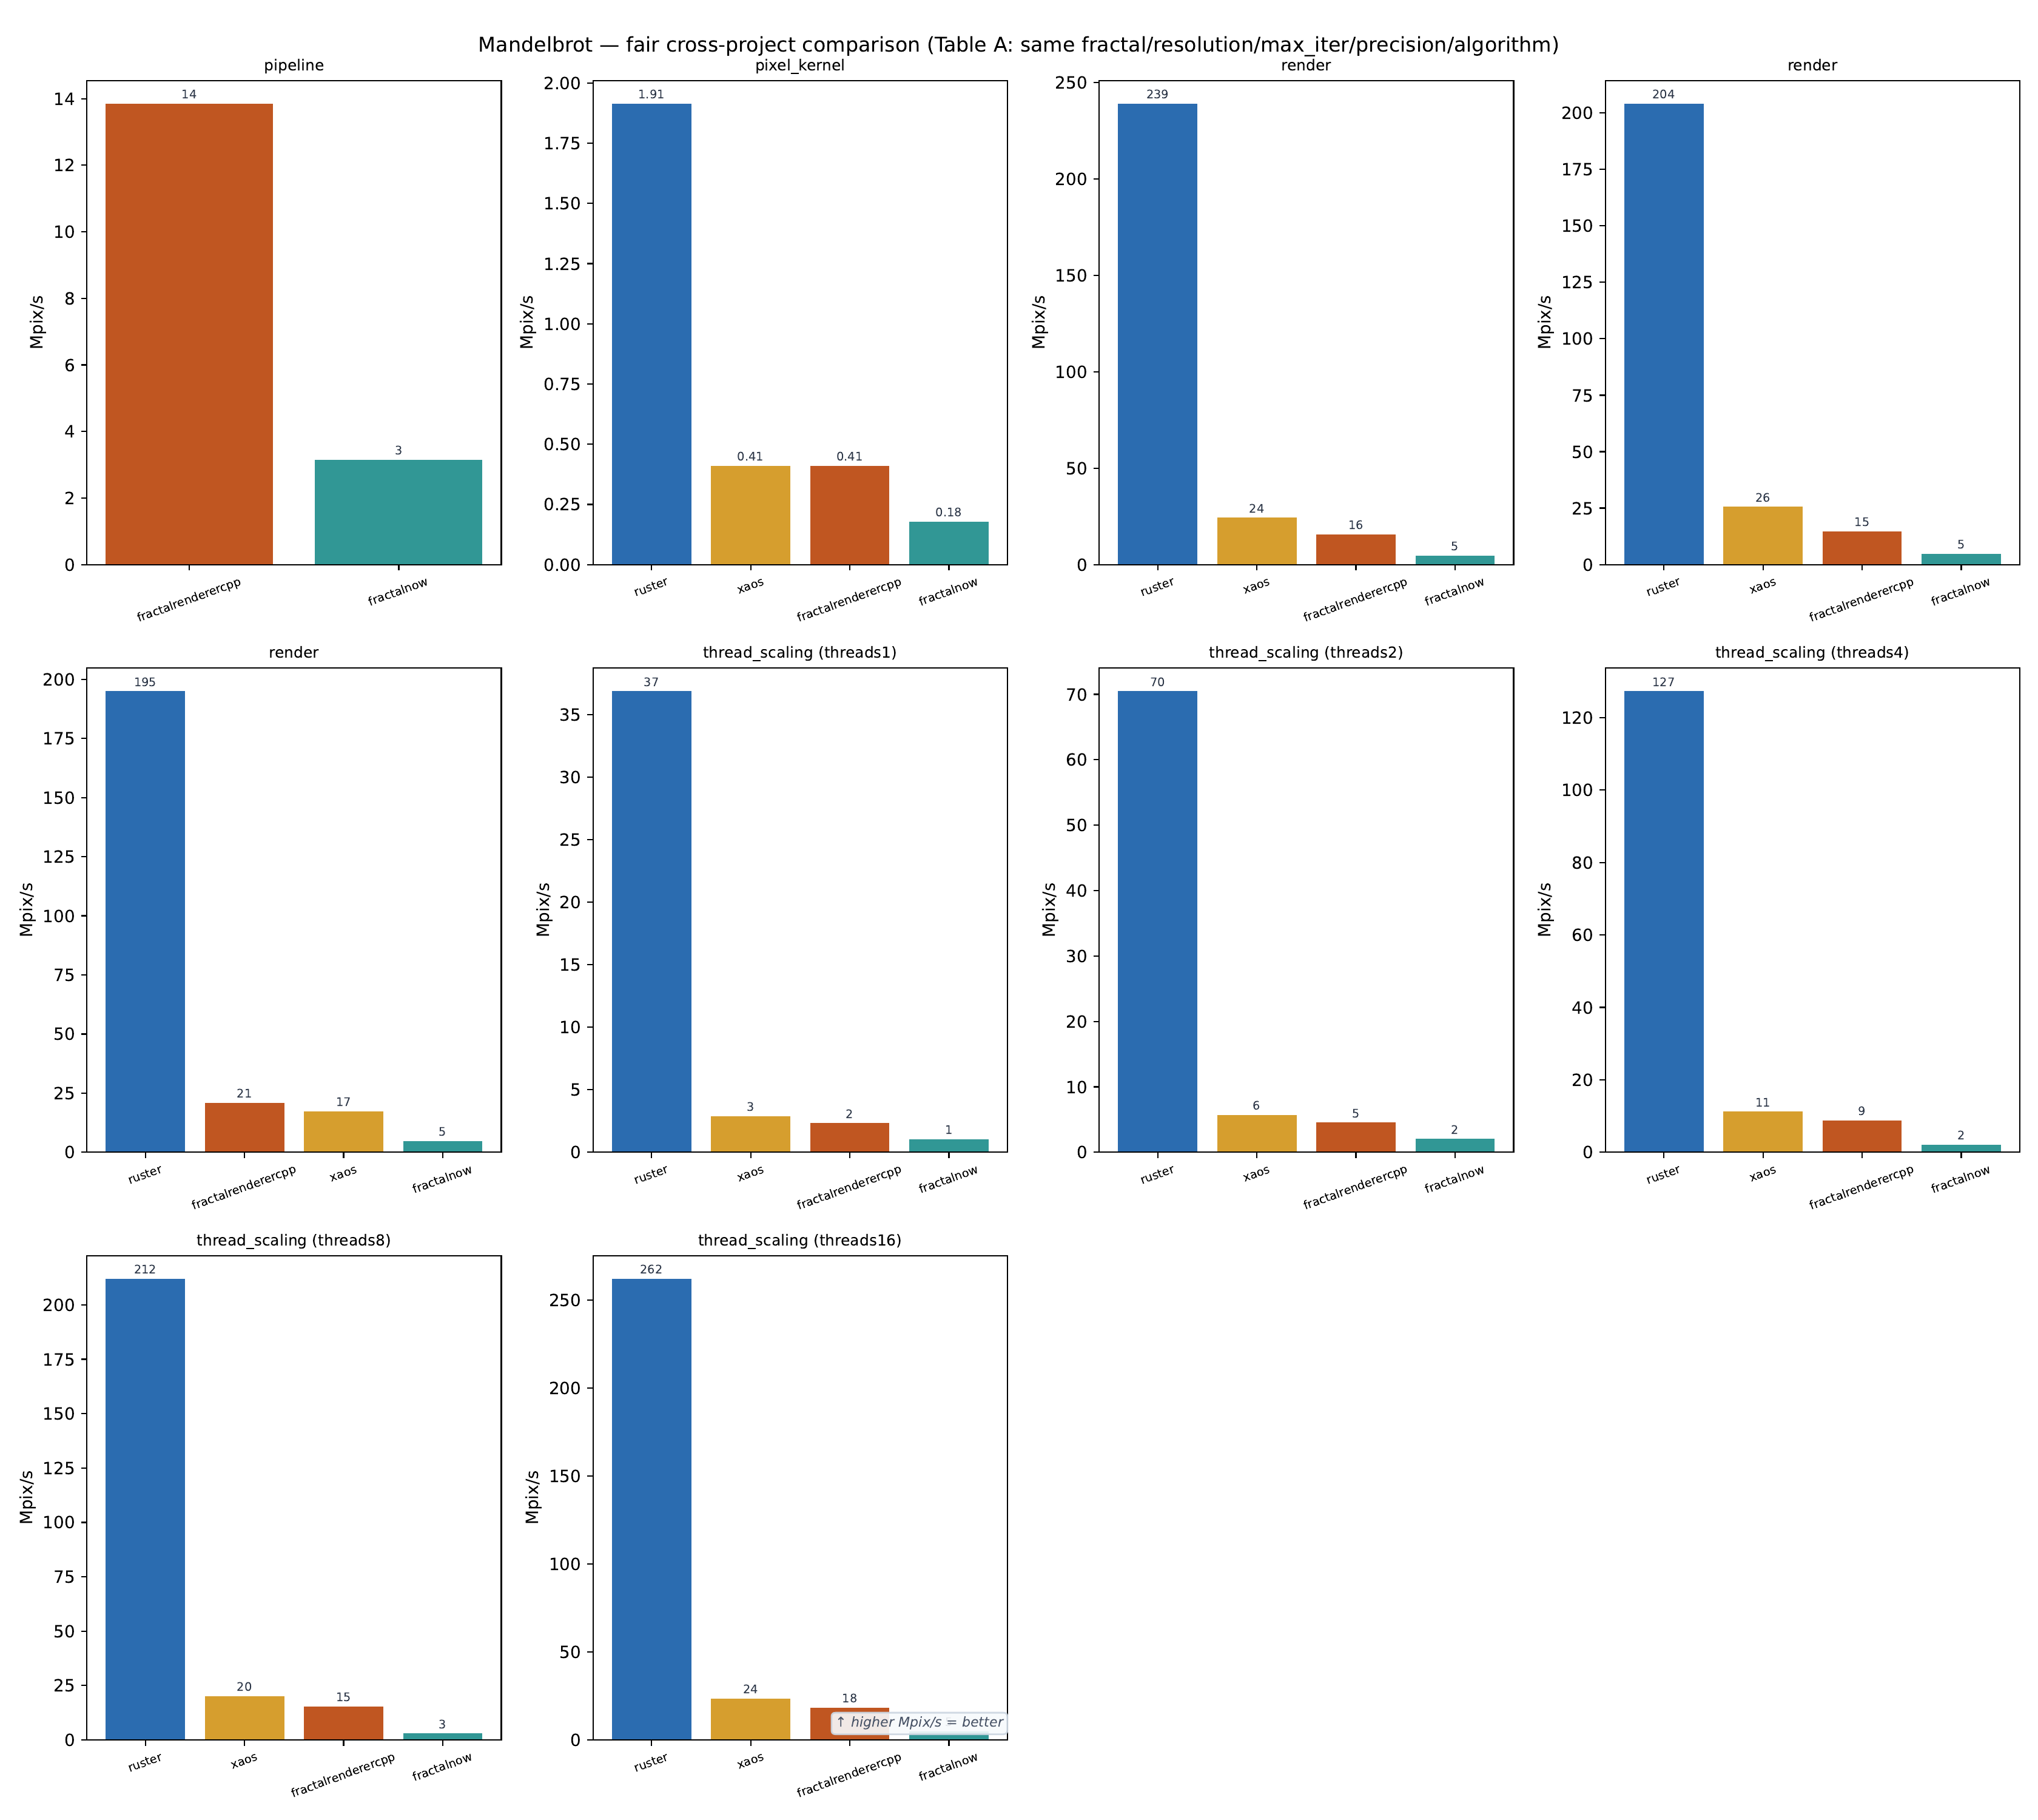
\includegraphics[width=\textwidth]{figures/ruster-cross-project-fair.png}
  \caption{Fair cross-project comparison, matched fractal, resolution,
  \kod{max\_iter}, precision, and algorithm class.}
  \label{fig:results-cross-project}
\end{figure}

Figure~\ref{fig:results-pixel-kernel} isolates just the per pixel kernel,
normalized to evaluations per second so that ruster's multi sample point
calls and the other projects' single point calls remain comparable, as
Section~\ref{sec:technology-stack} explains. ruster's kernel evaluates
roughly $4.7\times$ faster than XaoS's raw kernel, its own real time
boundary tracing forced off, and by coincidence lands at almost exactly
the same margin, roughly $4.7\times$, over FractalRendererCpp's, whose
bailout test resquares $z$ instead of reusing the update step's own
intermediates. FractalNow's raw kernel, quad interpolation forced off, is
slowest of the four, a generic macro generated dispatch layer, as
Section~\ref{sec:bench-cross-renderer} explains, rather than any specific
algorithmic shortfall.

\begin{figure}[H]
  \centering
  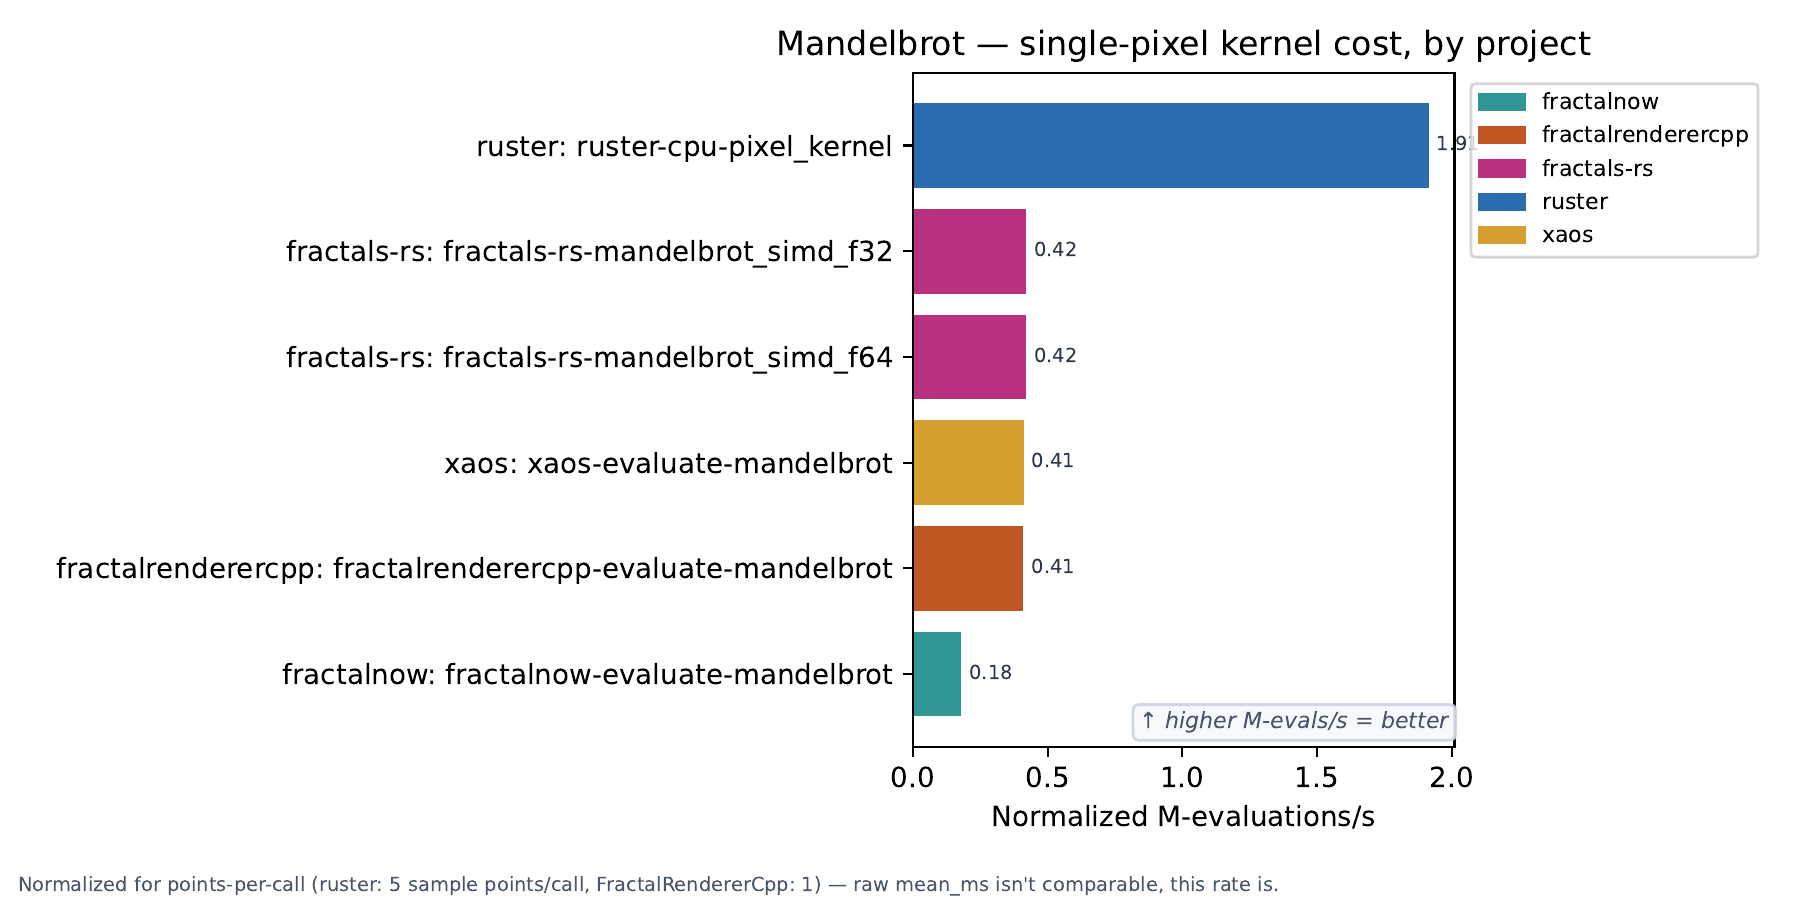
\includegraphics[width=0.8\textwidth]{figures/ruster-pixel-kernel-cost.png}
  \caption{Single pixel kernel cost, four projects, Mandelbrot, normalized
  M-evaluations/s.}
  \label{fig:results-pixel-kernel}
\end{figure}

The single threaded comparison against FractalRendererCpp, the fairest
pairing available since it controls for thread count, precision, and
algorithm class simultaneously, reaches $15.9\times$, $56.2$ against
$893.0\,\mathrm{ms}$, not from a language advantage but from ruster's
kernel already carrying the cardioid, period 2, and period 3 rejection
tests and Brent cycle detection that FractalRendererCpp's naive loop has
none of. Figure~\ref{fig:results-other-projects} shows the corresponding
resolution sweep for FractalRendererCpp on its own, throughput flat
within noise across all three resolutions, the same embarrassingly
parallel signature Section~\ref{sec:metrics-throughput} defines.
Fractals-rs, run in the same session as the other four, is SIMD only and
shows the same flat signature on both of its precision paths. Its
\texttt{fast} f32 path runs $811$ to $1113\,\mathrm{Mpix/s}$ across the
sweep and its \texttt{high} f64 path $417$ to $514\,\mathrm{Mpix/s}$,
each within noise of itself at every resolution rather than trending
with frame size.

\begin{figure}[H]
  \centering
  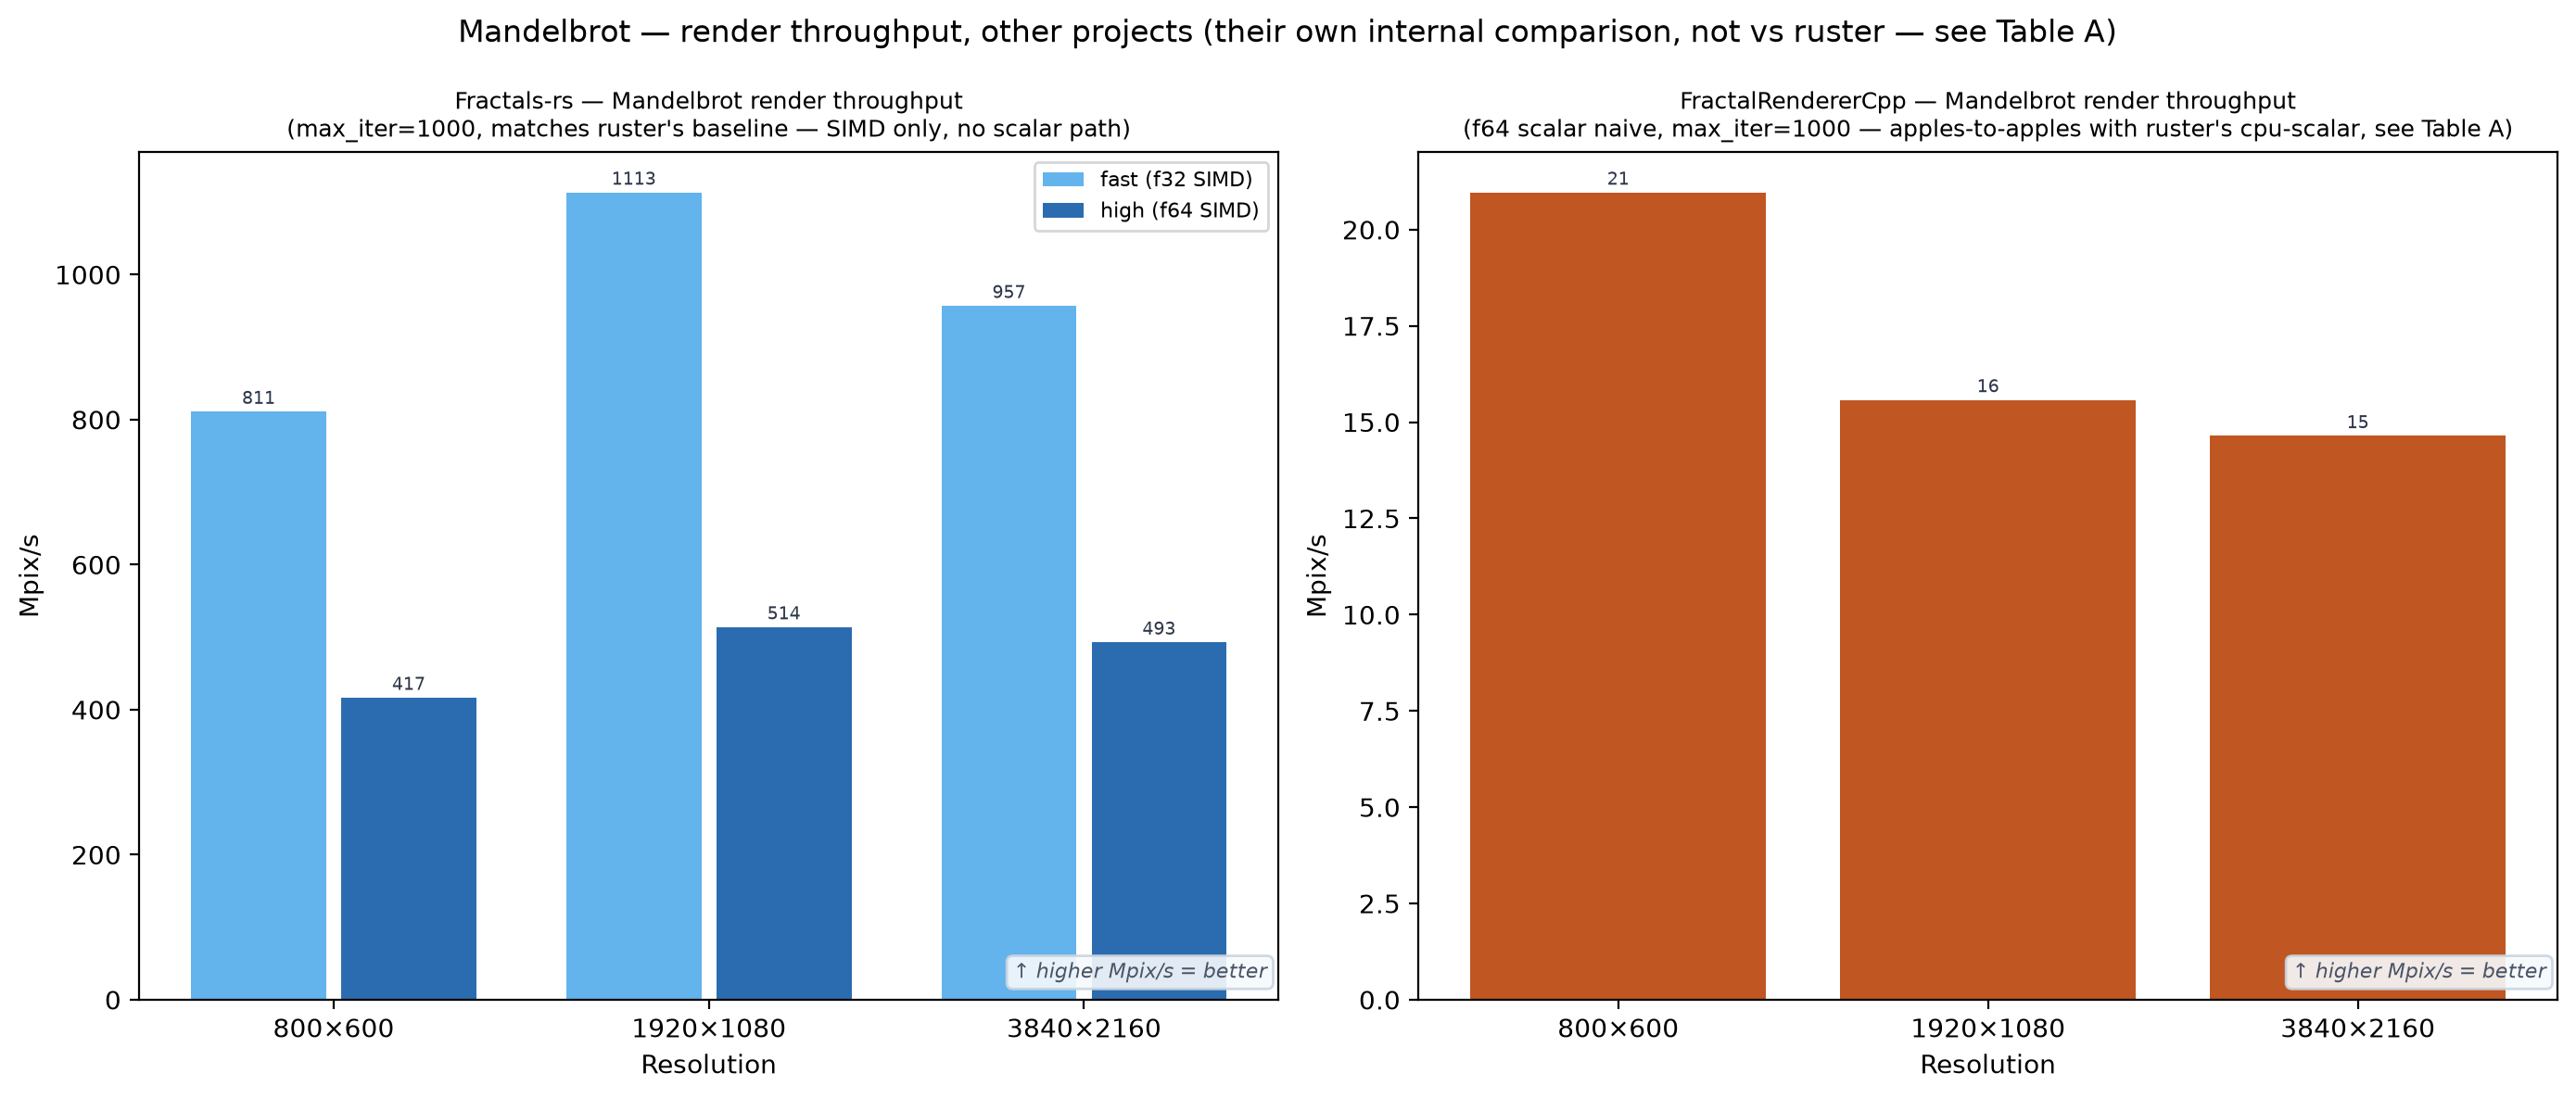
\includegraphics[width=0.75\textwidth]{figures/ruster-other-projects-internal.png}
  \caption{Fractals-rs's own resolution sweep, f32 vs f64 SIMD, and
  FractalRendererCpp's own resolution sweep.}
  \label{fig:results-other-projects}
\end{figure}

Every comparison in this section has been about speed. The next one asks
a question speed alone cannot answer, which of ruster's own two backends
is cheaper to run.

\FloatBarrier

\section{Energy Efficiency}
\label{sec:results-energy}

Figure~\ref{fig:results-energy} answers a question frame time alone
cannot, which device is cheaper to run, not just faster. The GPU reaches
$54.37$ GFLOPS at $13.49\,\mathrm{W}$ against the CPU's $100.35$ GFLOPS at
$33.82\,\mathrm{W}$, so the CPU wins on raw throughput but the GPU is
roughly $36\%$ more efficient per watt, $4.03$ against $2.97$ GFLOPS/W.
Faster and more efficient are answers to different questions on this
hardware, and a deployment optimizing for battery life or thermal budget
rather than latency would read this figure differently than the rest of
this chapter does.

\begin{figure}[H]
  \centering
  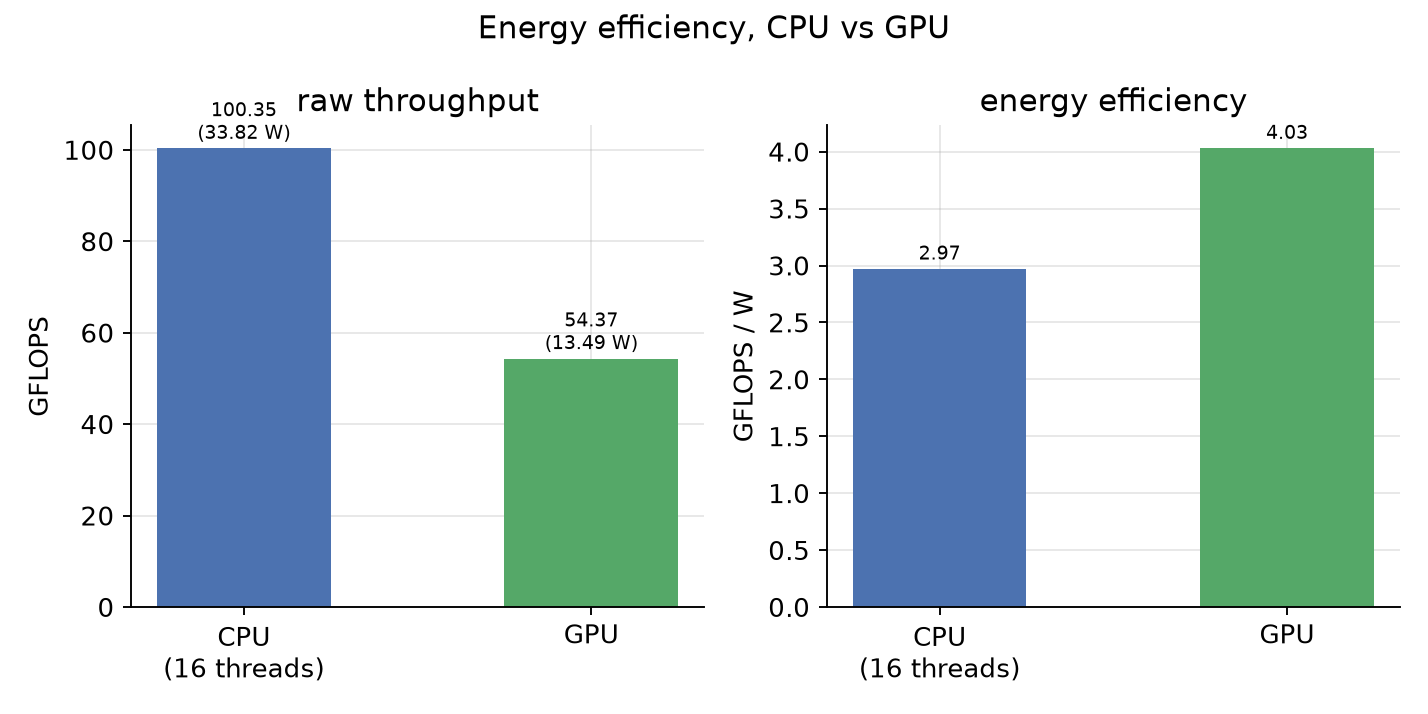
\includegraphics[width=0.95\textwidth]{figures/results-energy.png}
  \caption{Energy efficiency, CPU vs GPU, raw GFLOPS and GFLOPS per watt.}
  \label{fig:results-energy}
\end{figure}

\FloatBarrier

\section{Numerical Validation}
\label{sec:results-validation}

Every earlier section in this chapter asked how fast the renderer is.
This one asks whether it is still right. Chapters~\ref{ch:algorithms}
through~\ref{ch:scheduler} rewrote the same hot loop a dozen times over,
scalar to SIMD, CPU to GPU, direct iteration to perturbation, and a fast
renderer that quietly computes the wrong set would be worse than a slow
one, since nothing in a rendered image says how wrong it is. This section
checks two properties of the Mandelbrot set that do not depend on any
implementation choice, only on the mathematics from
Section~\ref{sec:mandelbrot-definition}, and closes the chapter by
confirming that every optimization measured so far changed speed and
nothing else, the correctness class Section~\ref{sec:correctness-metrics}
sets apart from the rest of this chapter.

Figure~\ref{fig:results-validation}'s left panel
fits a box counting dimension to the rendered boundary, $D\approx1.10$
with $R^2=0.9907$, well below the boundary's known Hausdorff dimension of
exactly $2$, the value Section~\ref{sec:mandelbrot-definition} gives, the
expected gap since the asymptotic value needs boundary detail at scales
finer than any finite render can reach. The right panel sweeps
\kod{max\_iter} against the Mandelbrot set's literature area estimate,
roughly $1.50659177$, and shows the error shrinking monotonically as the
cap grows, exactly as the escape time approximation in
Section~\ref{sec:escape-time-basics} predicts, since a cap that is too
small misclassifies slow escaping boundary pixels as interior and
inflates the estimate. Neither result depends on any optimization in
Chapter~\ref{ch:algorithms}, both come from the plain scalar kernel, and
both give the qualitative answer a differently implemented renderer
would, evidence that the optimizations elsewhere in this thesis changed
speed and not correctness.

\begin{figure}[H]
  \centering
  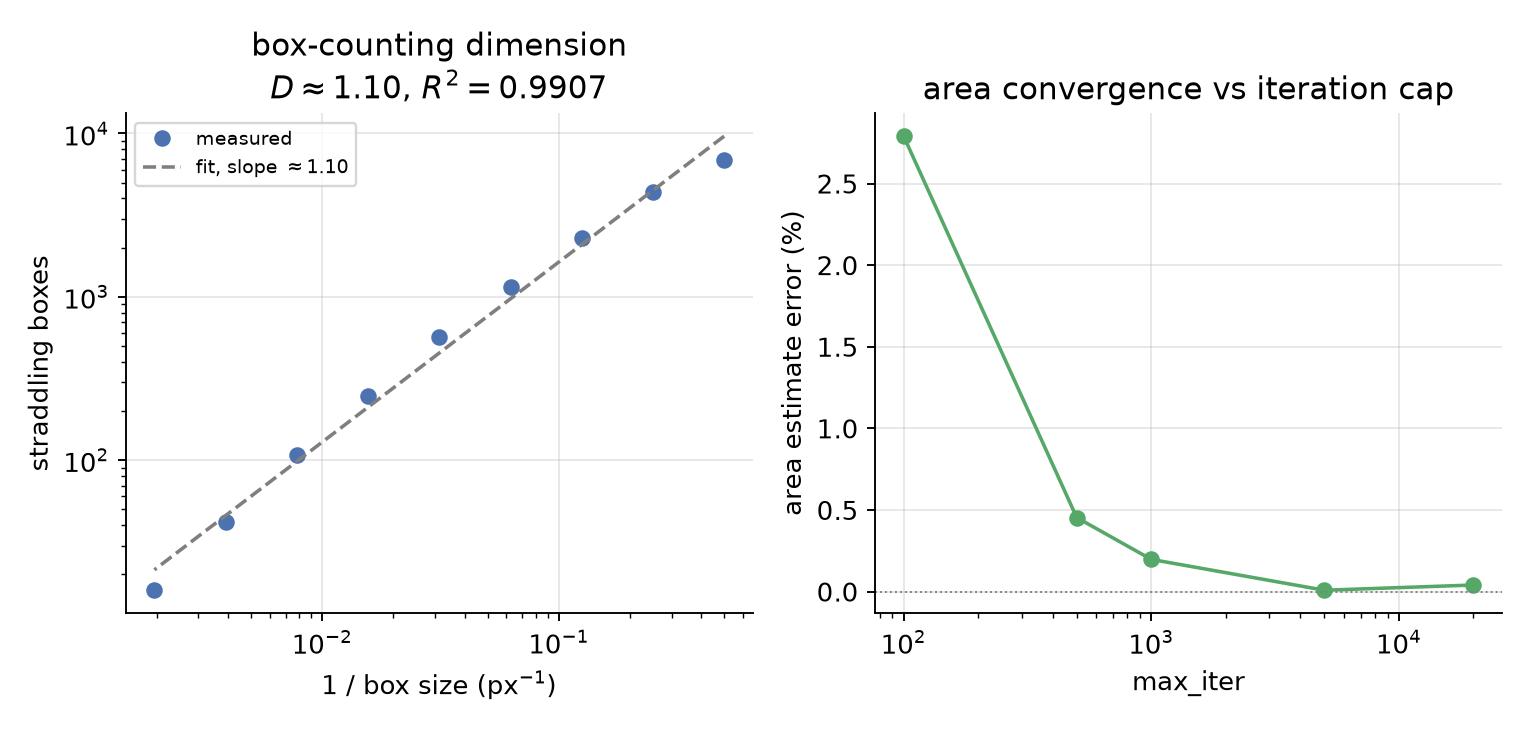
\includegraphics[width=\textwidth]{figures/results-numerical-validation.png}
  \caption{Numerical validation, box counting dimension of the rendered
  boundary and area estimate convergence against the iteration cap.}
  \label{fig:results-validation}
\end{figure}

Both checks land where the mathematics says they should, independent of
any speed result in the rest of this chapter. What the preceding sections
measured as throughput, then, was always throughput on the correct
answer.

\FloatBarrier

\chapter{Conclusion}
\label{ch:conclusion}

This thesis set out to answer a question that most fractal renderers
never actually ask. A typical personal computer has both a multicore CPU
and a GPU sitting idle for most of a render, so why settle for one? The
goal was to build a renderer that pushes a CPU path and a GPU path each
as far as they individually go, and then to tie the two together with a
scheduler that decides at runtime, tile by tile, which device should
render what, rather than assuming the split in advance. The expectation
going in was that the CPU path would need real optimization work before
it was a fair partner for the GPU at all, that the GPU would win outright
once that work was done, and that a scheduler would only earn its
complexity where the two devices were closely enough matched for the
choice of which one does what to actually matter. All three expectations
held, though not always for the reasons assumed at the start, and the
measurements in Chapter~\ref{ch:results} are the record of where the
guesses were right and where they were not.

The CPU side turned out to matter more than expected. A scalar baseline,
carried through rayon parallel threading and then SIMD, reaches roughly a
$1.9\times$ to $2.4\times$ speedup on its own depending on frame size,
but the bigger win came from a cheaper idea, testing whether a pixel is
provably inside the set before iterating it at all. That early exit
test, plus catching cycles the naive loop would otherwise burn iterations
on, is what let a single CPU thread outrun a comparable C++ renderer by a
factor of roughly sixteen, with neither side touching a GPU. Not
everything paid off. Hilbert curve traversal, chosen for its cache
locality properties, was slower than a plain row major scan at every
resolution tested, and perturbation theory, built for deep zoom, never
won a single benchmark within the zoom range this thesis actually
measured, because plain double precision arithmetic simply never broke
down in that range.

The GPU delivered on its promise of raw throughput, reaching roughly
$1389$ million pixels a second at 4K, well ahead of every CPU
configuration. What was not expected going in was where the GPU actually
spends its time. The two GPU backends' compute kernels are within five
percent of each other, and almost the entire gap between them comes from
copying the finished image back to the CPU, not from computing it.
Coloring the image afterward mattered more than the GPU versus GPU
comparison itself. Measured with colorize still running on the CPU for
both backends, that one step alone cut the GPU's advantage over the CPU
to well under half of its render only lead. Moving it onto the GPU turned
out to be the single largest performance gain this thesis identified, and
for CUDA the thesis went on to implement it, an on device histogram and
palette lookup kernel, pixel exact against the CPU version, $54\%$ to
$63\%$ faster end to end at the shallow and mid zooms where colorize
used to dominate frame time. wgpu and the heterogeneous scheduler still
colorize on the CPU, the scheduler by necessity since its merged buffer
only ever exists on the host side, so that gain remains a clearer
direction for future work on those two paths.

The hybrid scheduler is the part of this thesis with the most story to
tell. At a shallow zoom, where the CPU and the faster GPU are not close
in speed, every version of the scheduler, adaptive or not, loses to
simply picking the faster device and using it alone. The scheduler earns
its complexity at the one point where the two devices actually become
comparable, the precision threshold where both fall back to slower,
higher precision arithmetic and end up within about $10\%$ of each
other's speed. There, routing expensive tiles to the CPU instead of
splitting the frame evenly beats not only the better device alone but
also the theoretical best a blind split could achieve, by a factor of
$1.75$. That result is the clearest evidence this thesis has for its
central claim, a scheduler that looks at the work before deciding who
does it is worth more than one that just assumes. The advantage shrinks
at deeper zoom levels, leaving real headroom the scheduler does not yet
recover.

Against four existing open source renderers, ruster's own kernel was
roughly one order of magnitude faster than the closest competitor and two
orders of magnitude faster than the slowest, and none of that margin came
from Rust as a language, since the same early exit and cycle detection
work behind the CPU numbers is what accounts for it. A GPU is not
automatically the right answer, either. It is markedly more efficient
per watt than the CPU here, but the CPU still wins on raw throughput,
so "faster" and "cheaper to run" point at different devices depending on
what is actually being optimized for. And underneath all of the speed
numbers sits a quieter but necessary result. A box counting estimate of
the rendered boundary and a convergence check against the set's known
area both land where the mathematics predicts they should, which is the
evidence that a dozen rewrites of the same hot loop changed how fast this
renderer is and nothing about whether it is correct.

Two directions follow directly from what this thesis measured rather
than from speculation. Moving image coloring onto the GPU is the highest
value change identified but not built, and tuning the scheduler's deep
zoom behavior would close a real, already quantified gap rather than
requiring a new idea. A third, smaller direction is honest bookkeeping.
Perturbation theory was never tested at the zoom depths it was actually
designed for, so its real payoff, as opposed to its measured absence of
one, is still an open question. None of the three require rethinking
anything in this thesis, only continuing it.

%% =====================================================================
%%  References
%%
%%  On first mention of a reference in the text, use \cite{key}. Entries
%%  themselves live in cite.bib (BibTeX); run bibtex/biber as part of
%%  the build (see comment at the top of this file).
%% =====================================================================
\bibliographystyle{plain}
\bibliography{cite}

\chapter*{Biography}
\addcontentsline{toc}{chapter}{Biography}

Name Surname was born on dd.mm.yyyy in City. They completed primary
school "..." and secondary school "...". After finishing secondary
school, they enrolled in the ... study programme at the Faculty of
Technical Sciences in Novi Sad, where they studied from 20XX to 20XX.

%% =====================================================================
%%  Key documentation information (required appendix)
%% =====================================================================
\KDIpage
\KWDpage

\end{document}
